\documentclass[degree=bachelor,tocarialchapter]{thuthesis}
% 选项
%   degree=[bachelor|master|doctor|postdoctor], % 必选,学位类型
%\degree=bachelor
%   language=[chinese|english], % 可选(默认:chinese),论文的主要语言
%   secret,                % 可选(默认:关闭),是否有密级
%   tocarialchapter,       % 可选(默认:关闭),章目录中使用黑体(这项表示同时打开下面两项)
%   tocarialchapterentry,  % 可选(默认:关闭),单独控制章标题在目录中使用黑体
%   tocarialchapterpage,   % 可选(默认:关闭),单独控制章页码在目录中使用黑体

% 所有其它可能用到的包都统一放到这里了,可以根据自己的实际添加或者删除。
\usepackage{thuthesis}
\usepackage{ IEEEtrantools }
\usepackage{pifont}% http://ctan.org/pkg/pifont
\usepackage{booktabs}

\newcommand{\cmark}{\ding{51}}%
\newcommand{\xmark}{\ding{55}}%
% 定义所有的图片文件在 figures 子目录下
\graphicspath{{figures/}}
%%%%%%%%%%%%%%%%边张行的一些自定义宏%%%%%%%%%%%%%
% 1. 将原文中“第1章”样式改变为“第一章”,并进行自动编号
\CTEXsetup[name={第,章},number={\chinese{chapter}}]{chapter}


%%%%%%%%%%%%%%%%%%%%%%%%%%%%%%%%%%%%%%%%%5
% 可以在这里修改配置文件中的定义。导言区可以使用中文。
\def\myname{边张行}

\begin{document}

%%% 封面部分
\frontmatter
\thusetup{
  %******************************
  % 注意:
  %   1. 配置里面不要出现空行
  %   2. 不需要的配置信息可以删除
  %******************************
  %
  %=====
  % 秘级
  %=====
  secretlevel={秘密},
  secretyear={10},
  %
  %=========
  % 中文信息
  %=========
  ctitle={清华大学学位论文 \LaTeX\ 模板\\使用示例文档 v\version},
  cdegree={工学硕士},
  cdepartment={计算机科学与技术系},
  cmajor={计算机科学与技术},
  cauthor={薛瑞尼},
  csupervisor={郑纬民教授},
  cassosupervisor={陈文光教授}, % 副指导老师
  ccosupervisor={某某某教授}, % 联合指导老师
  % 日期自动使用当前时间,若需指定按如下方式修改:
  % cdate={超新星纪元},
  %
  % 博士后专有部分
  catalognumber     = {分类号},  % 可以留空
  udc               = {UDC},  % 可以留空
  id                = {编号},  % 可以留空: id={},
  cfirstdiscipline  = {计算机科学与技术},  % 流动站(一级学科)名称
  cseconddiscipline = {系统结构},  % 专 业(二级学科)名称
  postdoctordate    = {2009 年 7 月——2011 年 7 月},  % 工作完成日期
  postdocstartdate  = {2009 年 7 月 1 日},  % 研究工作起始时间
  postdocenddate    = {2011 年 7 月 1 日},  % 研究工作期满时间
  %
  %=========
  % 英文信息
  %=========
  etitle={An Introduction to \LaTeX{} Thesis Template of Tsinghua University v\version},
  % 这块比较复杂,需要分情况讨论:
  % 1. 学术型硕士
  %    edegree:必须为Master of Arts或Master of Science(注意大小写)
  %             “哲学、文学、历史学、法学、教育学、艺术学门类,公共管理学科
  %              填写Master of Arts,其它填写Master of Science”
  %    emajor:“获得一级学科授权的学科填写一级学科名称,其它填写二级学科名称”
  % 2. 专业型硕士
  %    edegree:“填写专业学位英文名称全称”
  %    emajor:“工程硕士填写工程领域,其它专业学位不填写此项”
  % 3. 学术型博士
  %    edegree:Doctor of Philosophy(注意大小写)
  %    emajor:“获得一级学科授权的学科填写一级学科名称,其它填写二级学科名称”
  % 4. 专业型博士
  %    edegree:“填写专业学位英文名称全称”
  %    emajor:不填写此项
  edegree={Doctor of Engineering},
  emajor={Computer Science and Technology},
  eauthor={Xue Ruini},
  esupervisor={Professor Zheng Weimin},
  eassosupervisor={Chen Wenguang},
  % 日期自动生成,若需指定按如下方式修改:
  % edate={December, 2005}
  %
  % 关键词用“英文逗号”分割
  ckeywords={白癜风, 分割, 弱监督学习, 超像素},
  ekeywords={Vitiligo, segmentation, weakly-supervised, superpixels}
}

% 定义中英文摘要和关键字
\begin{cabstract}
      白癜风是一种常见的皮肤色素脱失病,影响全世界 0.5\% 到 1\% 的人群,该病的主要特征是在体表形成大小无规则的白斑皮损,是一种严重影响外貌美观的疾病。白斑面积是临床治疗效果的重要评价指标, 白癜风在评估方法上缺乏共识,这使得分析或比较不同研究的结果变得困难。
    
    因此,根据现存方法的一些缺点,如计算量大、操作繁琐、对拍摄器材要求高、只适用于强对比度的图片等,本文提出了一个高效、简单、鲁棒性强的白癜风区域分割方法,这将有助于推进白癜风的评价体系的客观化,标准化进程。且在一定的场景下, 该方法同样可应用于其他病种皮损区域的分割。
   
     本文通过收集1000 张来自临床和网络的白癜风图片,制作了到目前为止最大的一个白癜风数据集 Vit2019,并且均进行了白癜风区域的像素级标注; 针对部分图像对比度低、皮损与正常皮肤过渡区域模糊等特点,提出了使用超像素分割方法作为图像预处理步骤,从而达到降低维度、剔除异常像素点、保留较完整准确的皮损边界等三个目的; 由于图像大小尺寸不一致,引出了经典超像素分割算法中初始种子点数目确定难的问题,并针对提出了改进的方法; 本文针对白癜风标注难的问题,提出了面向白癜风等色素性皮肤病的弱监督分割框架,将“既见森林,又见树木” 的策略应用于弱监督分割中,并将反馈思想与显著性传播过程相结合从而实现准确的分割。

    本文通过多个实验验证了该弱监督方法的有效性,并与强监督学习的实验结果进行对比,验证了在一些拍照环境恶劣、对比度很低的情况下,本文提出的弱监督方法可以更好的分割白癜风区域并保留白癜风的边缘细节。

\end{cabstract}

% 如果习惯关键字跟在摘要文字后面,可以用直接命令来设置,如下:
% \ckeywords{\TeX, \LaTeX, CJK, 模板, 论文}

\begin{eabstract}
    Vitiligo is a common skin pigmentation disease affecting 0.5\% to 1\% of the world. The main feature of this disease is the  irregular white spot lesions on the surface of the body, which is a serious affection of appearance. The area of white spot is an important evaluation index of clinical treatment effect. Due to lack of consensus on vitiligo evaluation methods, it is difficult to analyze or compare the results of different clinical treatments.
    
    Therefore, according to some shortcomings of the existing methods, such as huge computation cost, cumbersome operation, high requirements for shooting equipment, strictness for only strong contrast pictures, this paper proposes a vitiligo region segmentation framework with high efficiency, simplicity and robustness, which will help advance the objectification and standardization of the vitiligo evaluation system. 
    
    This paper porposed one of the largest vitiligo datasets, Vit2019, which has 1000 images of vitiligo from the clinical environment and the network, and all of which are pixel-levelly labeled;
    Due to the low image contrast and blurred transition area, superpixel is used as image preprocessing to reduce the feature dimension, eliminate an abnormal pixel, and retain a more complete and accurate skin lesion boundary;
     Due to the inconsistent image size, an improved method is proposed to tackle with the problem of determining the number of initial seeds in the classical superpixel algorithm;
  and this paper proposed a weakly supervised segmentation framework for pigmented skin diseases such as vitiligo. The innovative strategy of “seeing both forests and trees” for weakly supervised segmentation is applied and also, this paper explains how to apply feedback ideas to the process of saliency propagation.
    
   The effectiveness of the weakly-supervised framework is verified by several experiments, which proves that the proposed method can even better segment the vitiligo region in some cases where the shooting environment is poor and the contrast is low. Surprisingly, the proposed method is also able to keep the edge details of the vitiligo better.
    
\end{eabstract}


% 如果使用授权说明扫描页,将可选参数中指定为扫描得到的 PDF 文件名,例如:
% \makecover[scan-auth.pdf]
\makecover

%% 目录
\tableofcontents

%% 符号对照表
%\begin{denotation}[3cm]
\item[HPC] 高性能计算 (High Performance Computing)
\item[cluster] 集群
\item[Itanium] 安腾
\item[SMP] 对称多处理
\item[API] 应用程序编程接口
\item[PI] 聚酰亚胺
\item[MPI] 聚酰亚胺模型化合物,N-苯基邻苯酰亚胺
\item[PBI] 聚苯并咪唑
\item[MPBI] 聚苯并咪唑模型化合物,N-苯基苯并咪唑
\item[PY] 聚吡咙
\item[PMDA-BDA]	均苯四酸二酐与联苯四胺合成的聚吡咙薄膜
\item[$\Delta G$] 活化自由能 (Activation Free Energy)
\item[$\chi$] 传输系数 (Transmission Coefficient)
\item[$E$] 能量
\item[$m$] 质量
\item[$c$] 光速
\item[$P$] 概率
\item[$T$] 时间
\item[$v$] 速度
\item[劝学] 君子曰:学不可以已。青,取之于蓝,而青于蓝;冰,水为之,而寒于水。木
  直中绳。輮以为轮,其曲中规。虽有槁暴,不复挺者,輮使之然也。故木受绳则直,金就
  砺则利,君子博学而日参省乎己,则知明而行无过矣。吾尝终日而思矣,不如须臾之所学
  也;吾尝跂而望矣,不如登高之博见也。登高而招,臂非加长也,而见者远;顺风而呼,
  声非加疾也,而闻者彰。假舆马者,非利足也,而致千里;假舟楫者,非能水也,而绝江
  河,君子生非异也,善假于物也。积土成山,风雨兴焉;积水成渊,蛟龙生焉;积善成德,
  而神明自得,圣心备焉。故不积跬步,无以至千里;不积小流,无以成江海。骐骥一跃,
  不能十步;驽马十驾,功在不舍。锲而舍之,朽木不折;锲而不舍,金石可镂。蚓无爪牙
  之利,筋骨之强,上食埃土,下饮黄泉,用心一也。蟹六跪而二螯,非蛇鳝之穴无可寄托
  者,用心躁也。—— 荀况
\end{denotation}



% % 也可以使用 nomencl 宏包:

% \printnomenclature[3cm]

% \nomenclature{HPC}{高性能计算 (High Performance Computing)}
% \nomenclature{cluster}{集群}
% \nomenclature{Itanium}{安腾}
% \nomenclature{SMP}{对称多处理}
% \nomenclature{API}{应用程序编程接口}
% \nomenclature{PI}{聚酰亚胺}
% \nomenclature{MPI}{聚酰亚胺模型化合物,N-苯基邻苯酰亚胺}
% \nomenclature{PBI}{聚苯并咪唑}
% \nomenclature{MPBI}{聚苯并咪唑模型化合物,N-苯基苯并咪唑}
% \nomenclature{PY}{聚吡咙}
% \nomenclature{PMDA-BDA}{均苯四酸二酐与联苯四胺合成的聚吡咙薄膜}
% \nomenclature{$\Delta G$}{活化自由能 (Activation Free Energy)}
% \nomenclature{$\chi$}{传输系数 (Transmission Coefficient)}
% \nomenclature{$E$}{能量}
% \nomenclature{$m$}{质量}
% \nomenclature{$c$}{光速}
% \nomenclature{$P$}{概率}
% \nomenclature{$T$}{时间}
% \nomenclature{$v$}{速度}



%%% 正文部分
\mainmatter
\chapter{绪论}
\section{引言}
白癜风是一种常见的皮肤色素脱失病,影响全世界0.5\%到1\%的人群,该病的主要特征是在体表形成大小无规则的白斑皮损,是一种严重影响外貌美观的疾病, 白斑面积是临床治疗效果的重要评价指标,白癜风在评估方法上缺乏共识,这使得分析或比较不同研究的结果变得困难。而测量白斑面积的基础则是准确将白斑区域分割出来。

传统的白斑面积测量方法有目测估算法、点估算法、宫格法等\cite{林瑶2002医学图像分割方法综述}。但是由于其主观性强,缺乏客观的衡量标准,逐渐被基于图像分析的测量方法所取代。例如,目测估算法通过医生的主观判断,将病人分为几个患病等级,从而实施治疗方案;点估算法与宫格法是将透明度的塑料薄片贴于患处表面,通过人工拓取患病区域进而测量患病面积。这些传统方法缺乏客观评估且操作繁琐。随着图像处理技术的发展,基于图像分析的测量方法可以做到非接触式测量,客观准确,但由于图片拍摄环境、拍摄器材、患者皮肤自身的色度等诸多因素的限制,做到将白癜风区域高效,准确的分割出来仍具有一定难度。如基于混合颜色空间的K均值聚类方法\cite{2006数字图像处理}采用将输入的RGB图像转转换到CIELAB、HSV、YCbCr空间中进行K均值聚类分割,但该方法需要同时在三个空间下进行聚类,计算量大,难以对分辨率高的图像进行有效的处理,且以像素点为最小单位进行分割;使用Photoshop或者其他图像处理工具对白癜风区域进行手动分割,标记边缘的方法,效果虽精确但操作繁琐;基于snake模型对白癜风皮损边缘进行提取的方法,要求先给定目标区域的初始轮廓,且算法对噪声较为敏感,且设备要求高。使用YCbCr颜色空间与Fuzzy C-Means (FCM) 聚类相结合的方法,虽然达到了不错的分割效果,但无法适应图片对比度较小的情况。

因此,根据现存方法的一些缺点,如计算量大,操作繁琐,对拍摄器材要求高,只适用于强对比度的图片等,本文提出了一个高效、简单、鲁棒性强的白癜风区域分割方法,这将有助于推进白癜风的评价体系的客观化,标准化进程。且在一定的场景下,改方法同样可应用于其他病种皮损区域的分割。

\section{研究现状}
\subsection{白癜风评价体系}
白癜风在评估方法上缺乏共识,这使得分析或比较不同研究的结果变得困难。早期,白癜风欧洲任务小组(VETF)\cite{taieb2007definition}和白癜风面积评分指数(VASI)\cite{Iltefat2004Parametric}提出了更准确的疾病严重程度指数和治疗评估标准。

VETF 是一个综合的评分系统,其从白癜风的范围、阶段及进展三个方面综合评价。白癜风的范围采用传统的“九分法”测量,以患者手掌为体表面积1\% 估算,将身体分为四个部分:头和颈部( 0 ~ 9\%) 、躯干( 0 ~ 36\%) 、上肢( 0 ~ 18\%) 、下肢( 0 ~ 36\%) 。手和足在评价白癜风范围时分别纳入到上肢和下肢中评价,但在评价白癜风的阶段和进展时,则作为独立部分单独评价。白癜风的阶段则参考伍德灯下检查的结果进行评估,分为四个等级。零等级:正常肤色( 区域内无脱色) ;一等级:不完全正常肤色( 包括斑点脱色,这一阶段的少许白色毛发不影响阶段评级) ; 二等级: 完全脱色( 这一阶段的少许白色毛发不影响阶段评级) ; 三等级: 完全脱色,并伴随部分毛发变白( < 30\%) ; 四等级: 完全脱色,并伴随毛发完全变白。% cite 白癜风评估方法VETFa 和VASI 的介绍 王禹
白癜风的进展则是通过比较自然光下与伍德灯下皮损的边界。分为三个等级:边界相似、进展期白癜风( 持续的脱色) 、恢复期白癜风( 持续的复色) 。

VASI的目的是使医生能测量患者不同时间复色、脱色情况及治疗后的疗效。以患者手掌为体表面积1\% 估算,患者身体被分为5个独立的部分: 手,上肢,躯干,下肢和足,来估算身体每个部位白斑的面积。在每一次统计的过程中,每一皮损按照脱色程度分为7 个等级:0\%,10\%,25\%,50\%,75\%,90\% 或100\%, 如图\ref{fig:chap1_VASI}所示。100\% 表示完全白化,0\%表示正常无脱色。将每一部分内的皮损面积(以手掌单位) 乘以脱色程度得到每一部分的得分,将每一部分得分相加构成了整个身体的VASI 得分( 0 ~ 100 分).

近些年,还有一些其他的方法在以上两种经典的方法的基础上被提出,他们基于精心设计的病情问诊流程,包括从患者和专家两方面来评估病变的面积和严重程度,从而实现了更好的评估者内部可靠性\cite{feily2014vitiligo,van2016development}。
\begin{figure}[htbp]
\begin{center}
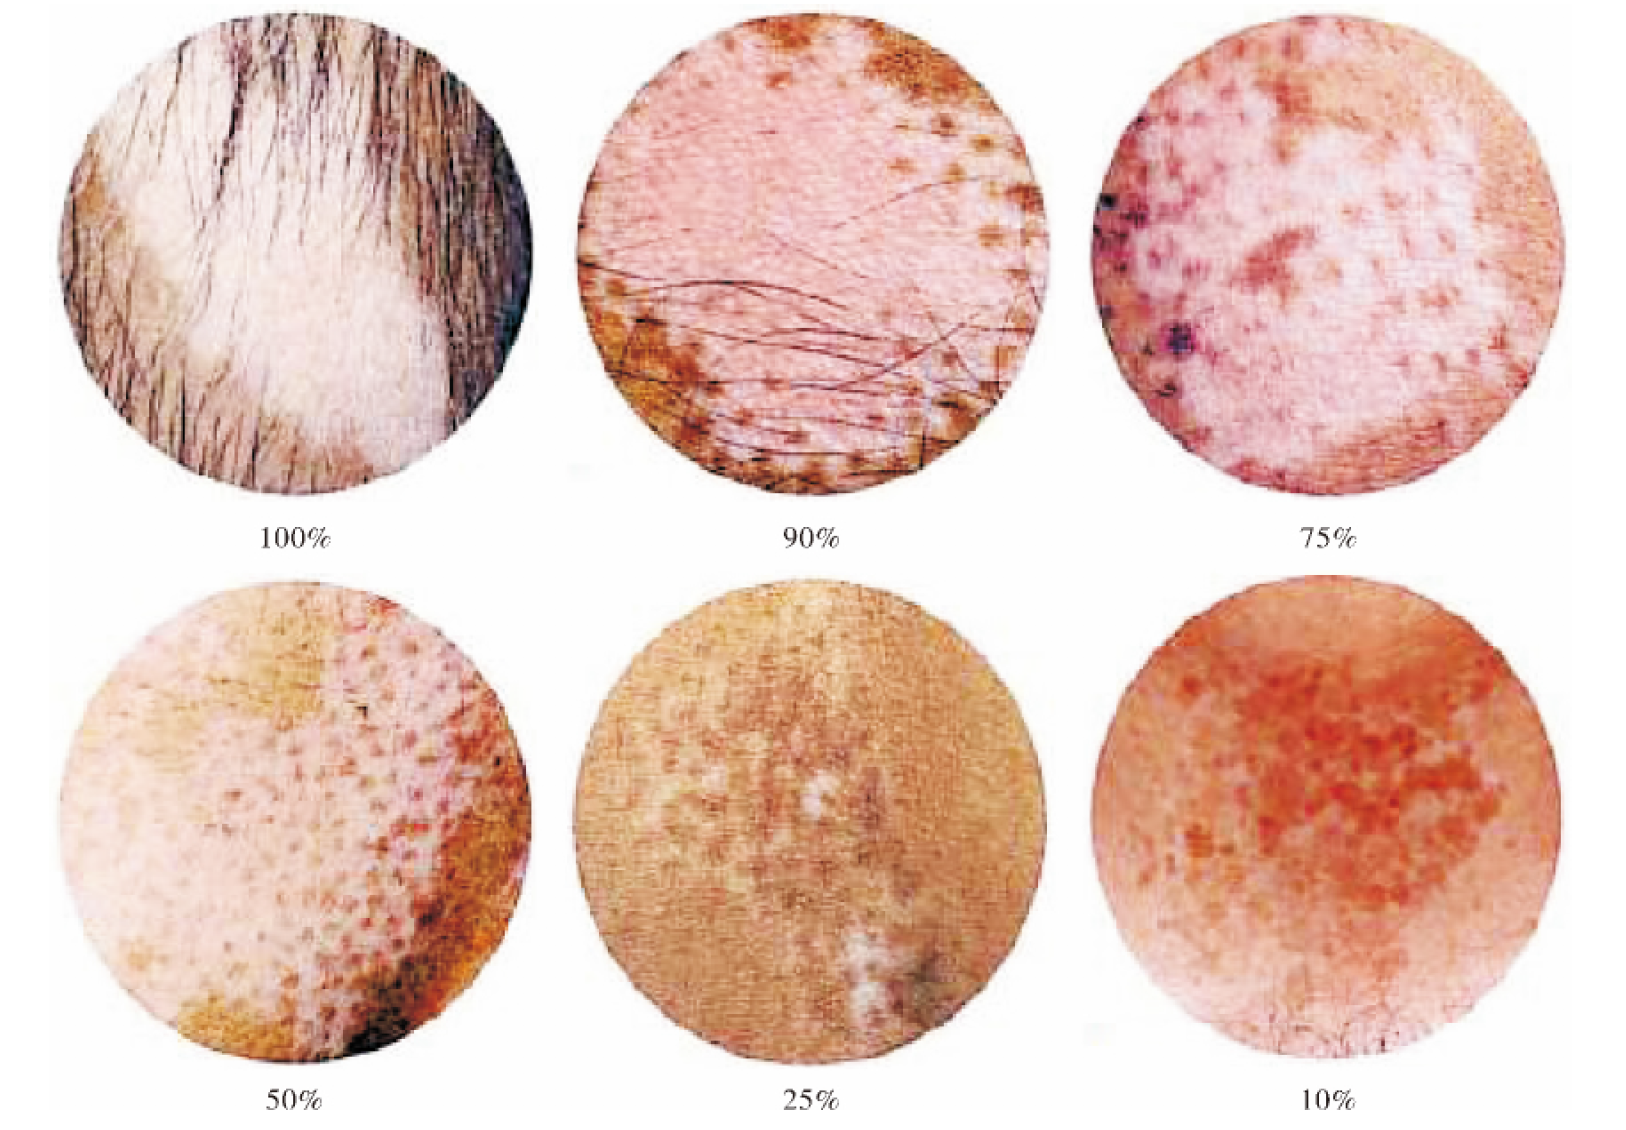
\includegraphics[width=0.7\linewidth]{chap1_VASI.png}
\end{center}
\caption{VASI指标白癜风脱色程度参考}
\label{fig:chap1_VASI}
\end{figure}
直到最近,研究人员才开始尝试以较少的人为干预来探索新的基于面积测量的评估,例如点计数方法,例如~\cite{aydin2007practical},planimetry~ \cite {aydin2007practical}和数字化方法\cite {marrakchi2008objective, verma2015evaluation}。但是,昂贵的设备和软件以及这些方法中的低效操作使其不太实用。例如,将透明薄片放置在白癜风病变上并用普通笔勾画边界,然后通过计算网格上的点或用CAD软件计算来测量该区域。因此,在产生大量图像的真实临床场景下应用这些方法是不实际的。

综上,本文发现目前所应用的白癜风评价体系大都是半客观的、基于专家或者病人本身的估算而评价的,难以做到客观评价。若要对其进行客观的评价,则需要精确的测量出白癜风边界的面积,而此前提便是对白癜风区域进行精确的分割。

\subsection{色素性皮肤病分割}
白癜风作为非常具有代表性的色素性皮肤病,其很多分割的方法都借鉴于色素性皮肤病的分割方法。

色素性皮肤病变图像分割的主流是基于边缘的方法、基于阈值的方法、基于区域的方法和深度学习方法。许多基于边缘的方法已应用于皮肤病变图像\cite {barcelos2009automatic,de2011skan}。然而,产生的边缘是不连续的并且对噪声敏感。阈值处理方法已被广泛应用于皮肤病变分割任务中\cite{norton2012three,abbas2013perceptually,cavalcanti2013coarse},此方法的原理较为直观,而且实现起来也很高效。但是对于对比度低的白癜风图像,该方法很难适用,因为难以选取准确的阈值边界。基于区域的增长、分裂和合并算法也已经被用于皮损区域的分割\cite{castillejos2012wavelet, de2011skan, wong2011automatic}。该方法的核心是选取一些种子点,然后采用一定的度量手段来对其周边的像素或者区域进行差异性度量,然后再采取合并或者分裂的操作。基于区域的方法已经显示出对图像噪声、不同的光照条件和低对比度的鲁棒性。
%其优点是实现相对简单,对于物体灰度值或其他特征值相差很大时,能很有效的对图像进行分割。其缺点是不适用于特征值相差不大的图像,对于图像中不存在明显的灰度差异或各物体的灰度值范围有较大重叠的图像分割问题难以得到准确的结果,这些方法可能产生比实际更小的片段并且导致非常不规则的病变边缘。增长区域算法、分裂和合并操作是典型的基于区域的技术,其特点是将分割过程分解为多个步骤,其中后续步骤要根据前面步骤的结果进行判断而确定。区域生长的基本思想是将具有相似性质的像素集合起来构成区域,该方法需要先选取一个种子点,然后依次将种子像素周围的相似像素合并到种子像素所在的区域中。这类方法已被用于分割皮肤病变\cite{castillejos2012wavelet, de2011skan, wong2011automatic}。


深度学习\cite{2010模式识别, 2016机器学习}已被应用于分割任务。例如人工神经网络\cite {schaefer2011colour, rajab2004application,2010模式识别},将图像分割问题转化为分类问题或者求解能量函数最小化等问题。其基本思想是用大规模数据集对网路进行训练,再用训练好的人工神经网络去分割。

近期,在人工神经网络的基础上有学者提出了完全卷积神经网络\cite{ 2018深度特征融合的图像语义分割, long2015fully, noh2015learning, ronneberger2015u}。完全卷积神经网络对图像进行像素级的分类,从而解决了语义级别的图像分割问题。与经典的卷积神经网络不同,完全卷积神经网络可以接受任意尺寸的输入图像,采用反卷积层对最后一个卷基层的特征图进行上采样,使它恢复到输入图像相同的尺寸,从而可以对每一个像素都产生一个预测,同时保留了原始输入图像中的空间信息。其中这种模型具有更快的速度和精确度。但其也存在相应的问题,例如数据集的获取需要大量的人工操作。从监督的角度上来看,不论是完全卷积神经网络还是人工神经网络,他们都需要大量的数据和监督信息,而在医疗图像领域,监督信息的获取又十分的困难。因此本文的贡献之一是提出了一种弱监督的分割方法,只需要利用图像的类别标签,即可完成对皮损区域的分割。

\subsection{白癜风图像的分析与分割}
针对白癜风的特点,一些学者也进行了一些研究。基于18名患者的41个白癜风区域的数字图像,Nugroho 等人 \cite {nugroho2013computerised}应用主成分分析(PCA),然后进行独立成分分析(ICA),分别将白癜风图像分为黑色素和血红蛋白成分两个成分。研究人员报告说,皮肤颜色是由于皮肤载色体组成,即黑色素和血红蛋白的组合。然而,在数字彩色成像中,通过组合三个光谱带产生颜色:红色,绿色和蓝色(RGB)。于是,在该算法中,主成分分析(PCA)用于将尺寸从三个(RGB)颜色通道减小到两个主要成分。接下来,ICA用于对齐两个主要成分轴以代表黑色素和血红蛋白,参见图\ref{fig:PCA}。然后白癜风皮肤区域被确定为缺乏黑色素的皮肤区域。在该方法中,首先确定一组种子点,然后使用区域增长算法,即从这些种子中,通过向每个种子附加具有与种子相似的属性的相邻像素来实现区域的增长。

\begin{figure}[htbp]
\begin{center}
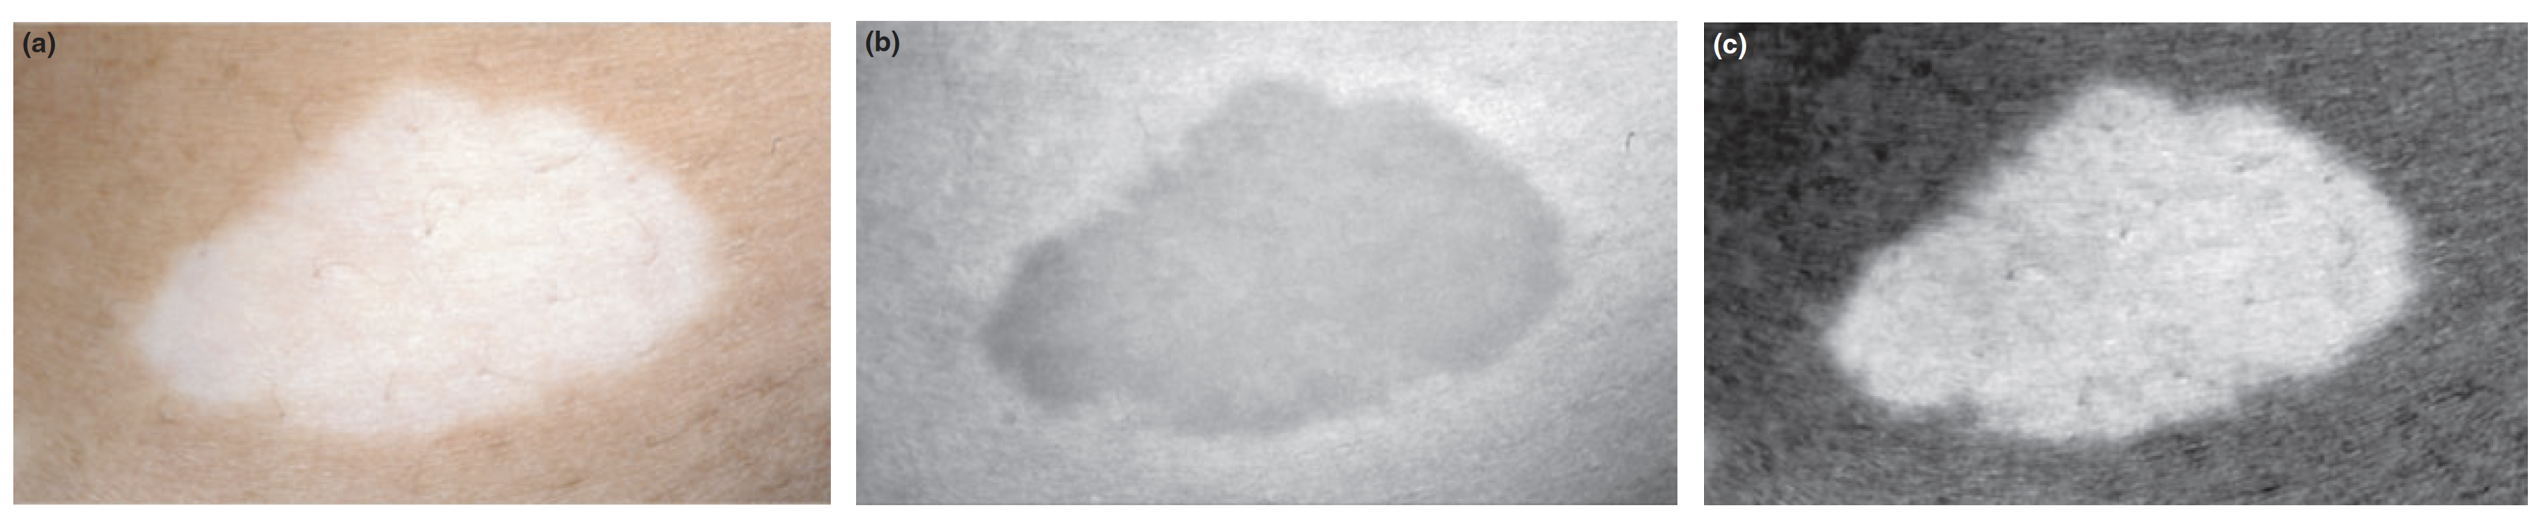
\includegraphics[width=\linewidth]{PCA.png}
\end{center}
\caption{PCA-ICA的例子。 (a)原始皮肤图像 (b)皮肤区域由血红蛋白引起的颜色(血红蛋白图像)(c)皮肤区域图像由黑色素引起的颜色(黑色素图像)}
\label{fig:PCA}
\end{figure}

但由于该方法所涉及的皮损区域较为简单,其算法在复杂场景不具备鲁棒性。但是其从医学方面分析白癜风形成的原因,这一角度为后面的研究提供了宝贵的经验。

Nurhudatiana 等人 ~ \cite {nurhudatiana2015computer}分别在YCbCr和RGB颜色空间的Cr和Blue通道中进行模糊C均值聚类,以分离图像中的背景、皮肤、皮损区域。 使用YCbCr颜色空间是因为YCbCr颜色空间中的CbCr二维平面的大Cr值的坐标非常好地定位了肤色。使用FCM算法是因为皮肤的像素倾向于在图像中形成均匀的簇,因此可以将皮肤分割作为聚类问题来处理。

\begin{figure}[htbp]
\begin{center}
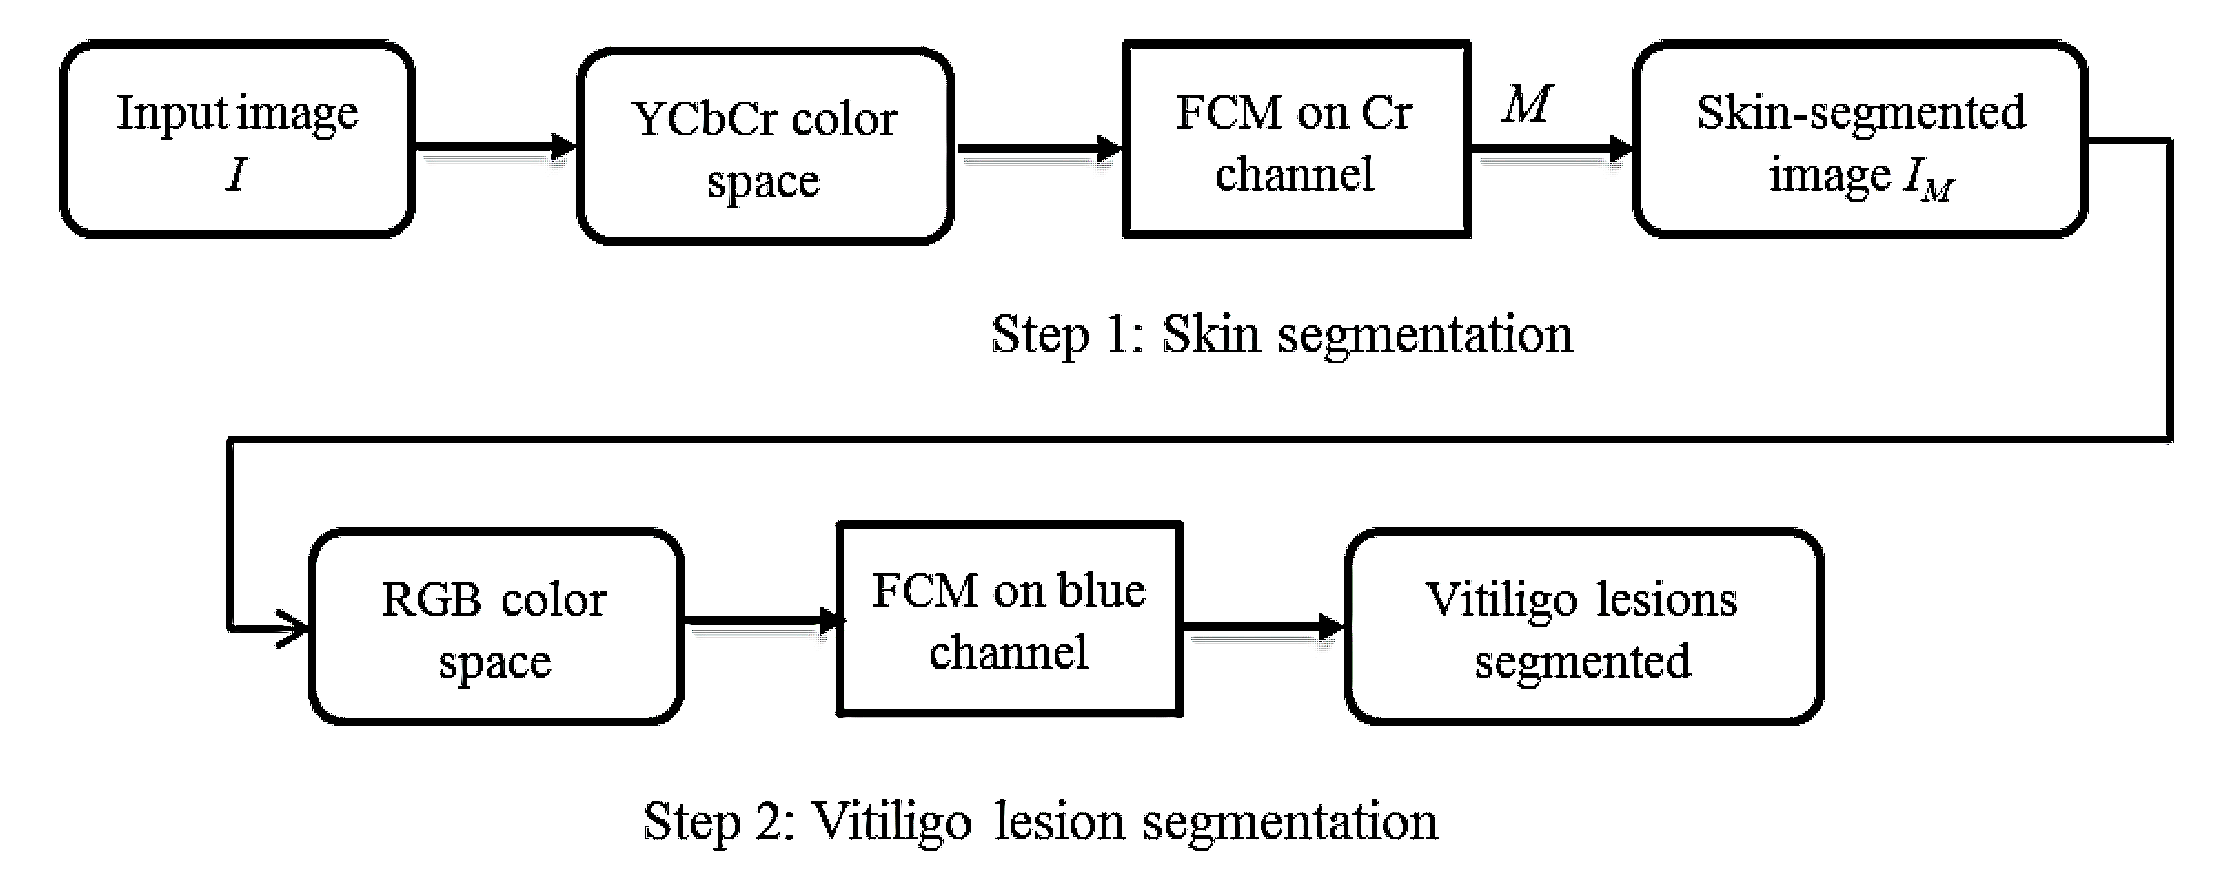
\includegraphics[width=0.9\linewidth]{FCM1.png}
\end{center}
\caption{结合YCbCr与FCM 方法流程图 \cite {nurhudatiana2015computer}}
\label{fig:FCM1}
\end{figure}

其所提出的算法如图\ref{fig:FCM1}所示。该算法由两个步骤组成。第一步是皮肤分割步骤,其用作预处理以定位图像中的皮肤区域,第二步是白癜风病变分割步骤。皮肤分割步骤的工作原理如下。给定输入RGB图像,首先将图像变换为YCbCr颜色空间以进行皮肤分割。然后使用均值滤波器提取和平滑Cr通道。然后使用模糊C均值(FCM)聚类算法将平滑后的通道分割成两个不同的聚类。由于皮肤趋向于在Cr通道中具有高强度值,因此以在通道Cr中10和90百分位的强度值的位置初始化聚类中心,其中第一簇表示背景,第二簇表示皮肤。该过程产生皮肤掩模M(参见图\ref{fig:FCM2})。

\begin{figure}[htbp]
\begin{center}
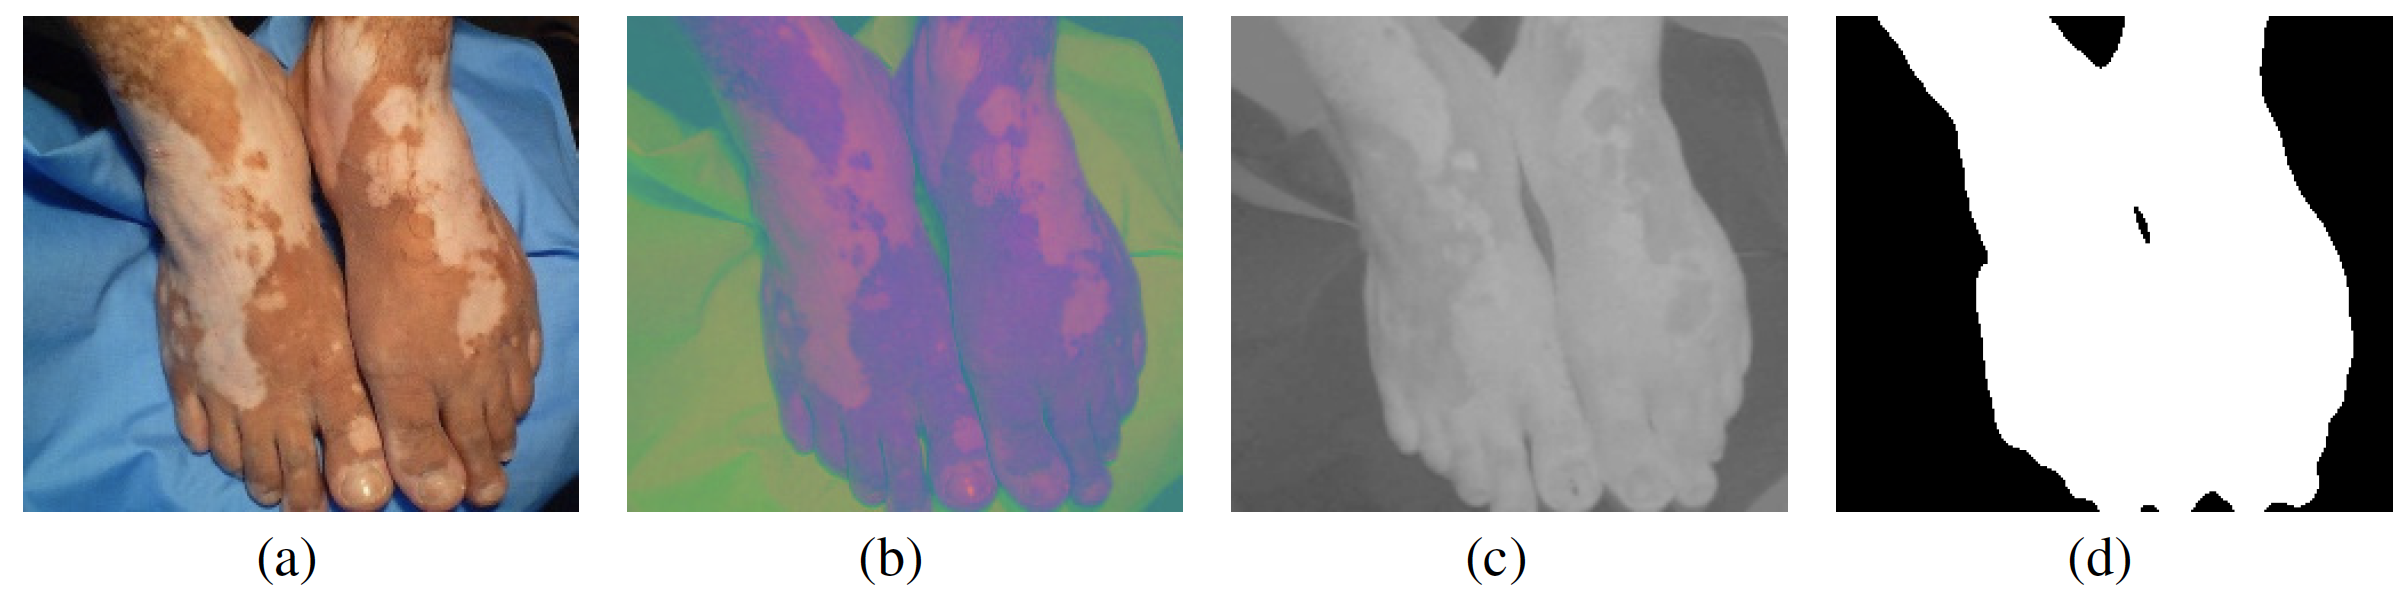
\includegraphics[width=0.9\linewidth]{FCM2.png}
\end{center}
\caption{皮肤分割过程 \cite {nurhudatiana2015computer}。(a) 输入RGB图像,(b) YCbCr颜色空间中的输入图像,(c) 从(b)中提取的Cr通道,以及(d)皮肤掩模$M$}
\label{fig:FCM2}
\end{figure}

然后使用形态学操作器平滑皮肤掩模$M$,该操作移除尺寸小于图像像素分辨率的10%的所有连通分量。将蒙版$M$应用于输入图像以获得皮肤分割图像$I_M$,其中属于第一聚类(背景)的像素的值被设置为零,并且属于第二聚类(皮肤)的像素的值被保留。经过皮肤分割后,还需要再进行白癜风皮损区域分割。在该步骤中,使用不同的颜色通道,尤其是RGB颜色空间的蓝色通道。蓝色通道波长接近紫外波长,而红色和绿色通道的波长穿透皮肤的较深层。因此,与红色通道和绿色通道波长相比,皮肤对蓝色通道波长更敏感。图\ref{fig:FCM3}比较了红色,绿色和蓝色通道中白癜风皮肤的外观。

\begin{figure}[htbp]
\begin{center}
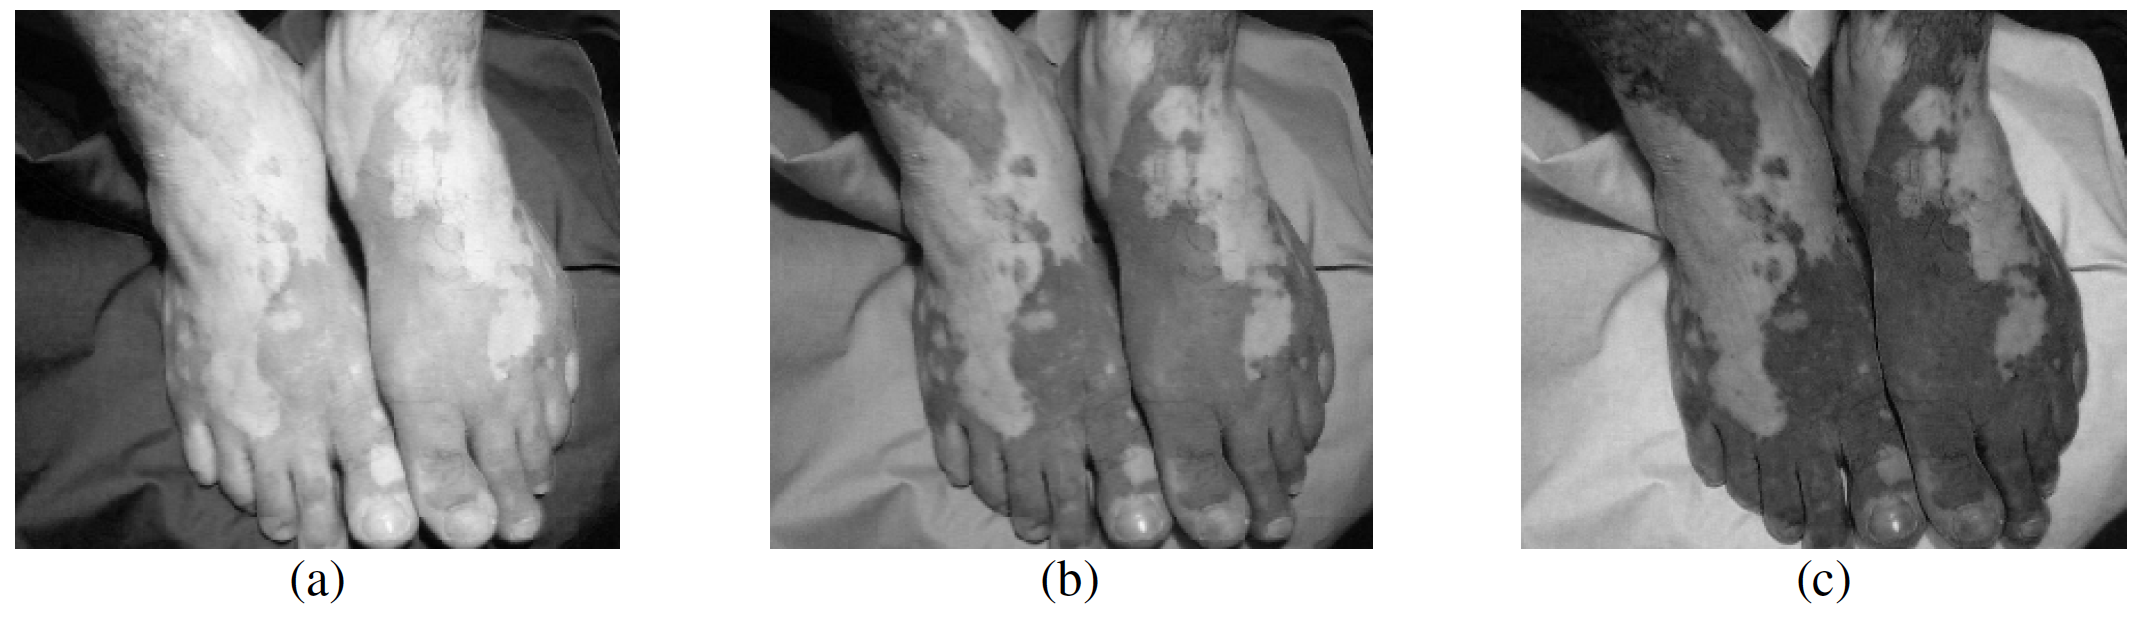
\includegraphics[width=0.9\linewidth]{FCM3.png}
\end{center}
\caption{白癜风皮观在(a)红色通道,(b)绿色通道和(c)蓝色通道中的比较 \cite {nurhudatiana2015computer}}
\label{fig:FCM3}
\end{figure}

可以观察到,与其他通道相比,正常皮肤和脱色皮肤之间的对比度差异在蓝色通道中最高(如图\ref{fig:FCM3}所示).然后同样将FCM聚类操作应用于分割好的皮肤图像。然后基于质心值进一步对得到的聚类进行分类。质心几乎等于零的簇表示黑色背景,因此在皮肤图中用黑色标记,而剩余的两个具有非零质心的簇表示皮肤。具有较低质心值的簇表示着色皮肤的像素,因此在皮肤图中用灰色标记,而具有较高质心值的簇表示脱色皮肤的像素,因此在皮肤图中用白色标记。

该方法利用白癜风对紫外线敏感的特征,对白癜风皮损区域达到了较好的分割效果。但是由于照片的拍摄环境不同,患者的皮肤肤色不同,会使得该先验知识在一定环境下失效。且方法中许多阈值需要人为手工确定,难以适应大量图像的自动化处理。

近些年来,还有一些基于超像素的分割方法,通过使用不同的视觉特征或超像素尺度聚合超像素。Mithun 等人~ \cite {das2015kl}提出了一种基于对称Kullback-Leibler散度的凝聚聚类方法,用于分割白癜风图像中的多种脱色水平,如图\ref{fig:KL1}。

\begin{figure}[htbp]
\begin{center}
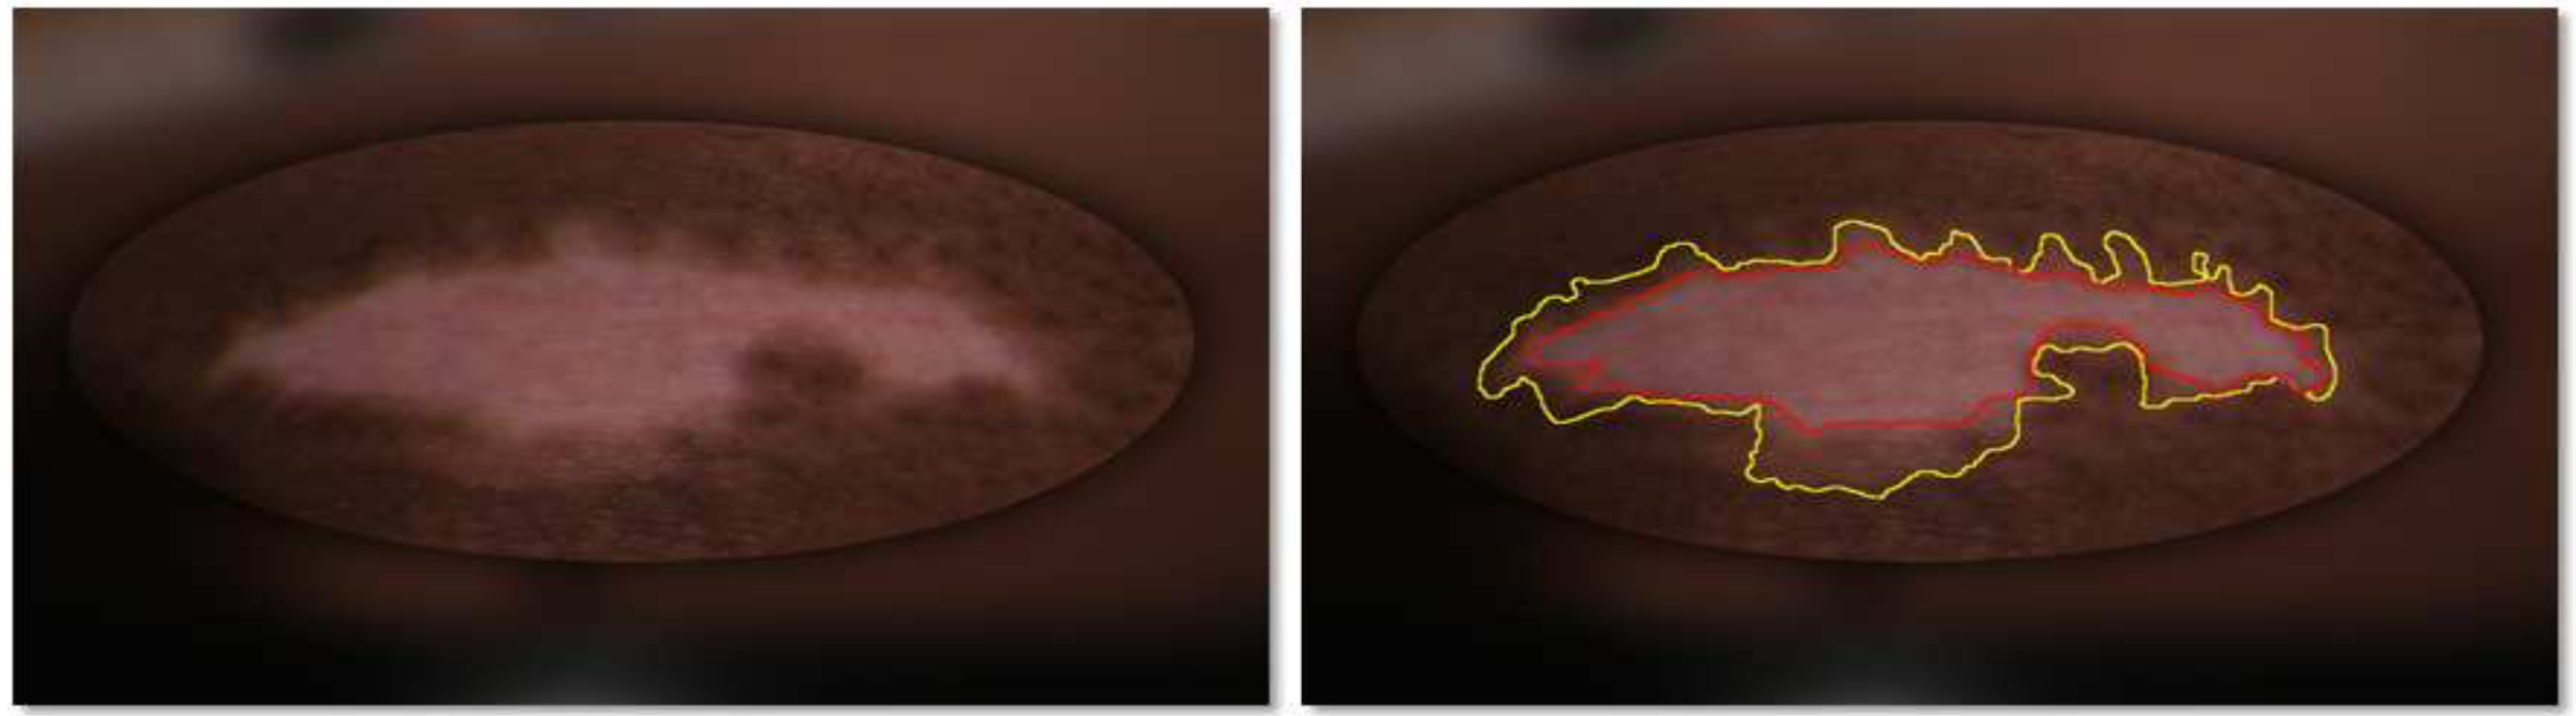
\includegraphics[width=0.9\linewidth]{intro.png}
\end{center}
\caption{⽩癜风分割及其专家标注\cite {das2015kl}。红⾊边界标志着完全脱⾊的⽪肤。黄⾊边界表⽰部分脱⾊的⽪肤。}
\label{fig:KL1}
\end{figure}

他们首先提出了两个正态分布的簇之间的对称Kullback-Leibler(KL)散度(等式\ref{eq:KL2}),作为距离度量。
\begin{IEEEeqnarray}{rCl}
\label{eq:KL1}
KL_{C_i,C_j}&=&\frac{1}{2}(tr({\Sigma_j^{-1}\Sigma_j^{-1}})+(\mu_j-\mu_i)^T\Sigma_j^{-1} \nonumber \\
&& (\mu_j-\mu_i)-d-\ln{\frac{|\Sigma_i|}{\Sigma_j}})
\end{IEEEeqnarray}
\begin{equation}
\label{eq:KL2}
D_{SKL}(C_i,C_j)=KL_{C_i,C_j}+KL_{C_j,C_i}
\end{equation}
其中$C_i$和$C_j$表示簇,$(\mu,\Sigma)$表示特征均值和协方差,d是特征维度。 对数项和逆协方差项在公式中是明显的瓶颈,这使得研究人员不使用基于KL散度的成本函数。 在协方差不为奇异的情景中,KL散度被证明是非常有用的散度度量。 对于基于区域的皮肤图像,特征上的协方差很少达到零。 此外,他们在协方差矩阵中加一个小分量\cite{Gupta2011Non},以保证迹的有界性。 

在这种对称的KL散度基础上,他们使用自下而上的分层凝聚聚类算法进行白癜风图像的分割。使用超像素作为图像基元图像特征,以降低后续图像处理任务的复杂性。他们观察到由于白癜风是一种表皮疾病,患者部分或完全丧失皮肤着色,这导致患病斑块的更高反射。于是将白癜风斑块分解成反照率区域和阴影区域图像。他们根据不同的脱色阶段,引入反照率和阴影图像作为白癜风区域分割的特征。其参照了 Zhu和Yuille\cite{zhu1996region}在关于区域竞争的论文中提出的用反照率图像进行皮肤图像分割的方法。

每个像素的特征向量具有十个维度,是由以下加权的矩阵堆叠而成。 记LAB为CIELAB彩色图像(3通道),RGB为彩色图像(3通道),A为反照率图像(3通道),S为阴影图像(3通道),$L=\Sigma_cI^c/\Sigma_cI$( 单通道)为图像的亮度。那么特征图像$I_f$就可以表示为:
\begin{equation}
\label{eq:2}
I_f
\begin{bmatrix}
LAB*(1+\gamma S))\\ 
\alpha RGB*(1+\gamma S))\\ 
\beta A*(1+\gamma S))\\ 
\kappa L
\end{bmatrix}
\end{equation}
其中$\alpha,\beta,\gamma$ 和 $\kappa$是自由参数,来加权不同的图像,$*$表示将每个通道相乘。 其算法思路见表\ref{tab:addlabel}
% Table generated by Excel2LaTeX from sheet 'Sheet1'
\begin{table}[htbp]
  \centering
   \caption{基于KL散度的图像分割层次聚类算法}
    \begin{tabular}{l}
    \toprule
    \textbf{算法1} 基于KL散度的图像分割层次聚类算法 \\
    \midrule
    \multicolumn{1}{p{28.2em}}{需要RGB彩色图像,最终聚类数量$c_F$生成反照率(A)和阴影(S)图像生成超像素} \\
    \textbf{重复} \\
    \hspace{1em}为集群生成邻接矩阵 \\
    \hspace{1em}计算特征空间中相邻超像素的成对亲和度 \\
     \hspace{1em}合并具有最低亲和力的两个群集并更新群集统计信息 \\
    \textbf{直到} 簇数等于 $c_F$ \\
    返回最终簇 \\
    \bottomrule
    \end{tabular}%
   
  \label{tab:addlabel}%
\end{table}%

然后设计了一种自上而下的聚类技术,将最后几个聚类合并到具有生理意义的标签上。但是对于不同图像的聚类停止规则难以统一。为了解决这个问题,他们为所有方法提出了一个停止准则,即$c_F = 15$,其中$c_F$在算法1中定义。

虽然该方法可以分割出不同脱色程度的白癜风区域。但是,对于一些较复杂在的情况,该方法仍然难以胜任,而且由于统一了自下而上聚类算法的停止准则,所以对不同图片的处理效果也良莠不齐。

综上,本文的方法相比于目前的皮损区域分割或者白癜风区域分割的方法,优势在于:
\begin{enumerate}
\item 无需任何人为干预的自动分割;
\item 基于弱监督的分割,无需做像素级别的人工标注。
\item 在不同环境下,分割效果具有很强的鲁棒性。
\end{enumerate}

\section{面临挑战}
在具体的临床应用中,我们往往会遇到很多实际的问题,而目前很多的研究方法均是在一些公开数据集上进行测试,由于公开数据集非常的干净且成熟,往往很难涵盖在实际应用场景下的出现的问题。就白癜风分割问题而言,如图\ref{fig:chap1_challenge}所示,这个任务具有以下难点:
\begin{enumerate}
\item 脱色和正常皮肤之间的低对比度、模糊的过渡区域; 
\item 临床拍摄中变化和不受控制的照明条件;
\item 一些干扰物体的存在 (例如,头发,反射,阴影和衣服); 
\item 在此方面缺乏大数据集用于数据驱动的模型 (例如,深度学习),而用于皮损区域的像素级标注的成本高昂。
\end{enumerate}
\begin{figure}[htbp]
\begin{center}
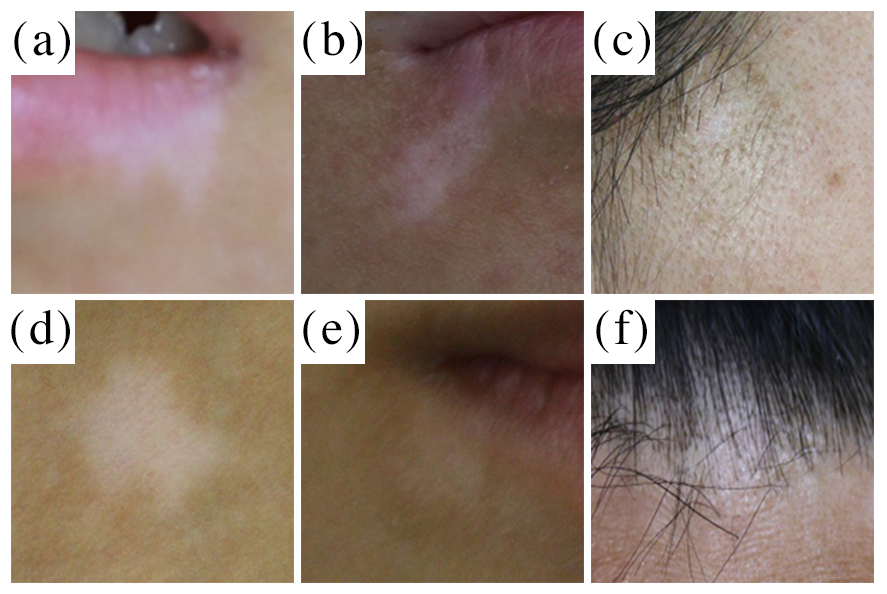
\includegraphics[width=0.7\linewidth]{chap1_challenge.jpg}
\end{center}
\caption{白癜风图像的例子和分割任务的挑战。}
\label{fig:chap1_challenge}
\end{figure}
如图\ref{fig:chap1_challenge},(a)-(d)展示了由于光照条件差和患者自身的肤色,皮损与健康皮肤之间的界限非常模糊。(e)对比度非常低。(c)和(f)都受到毛发的阻挡。由于(c)和(f)中的过渡曝光,部分健康皮肤容易被误认为是白癜风病变。

以上的各个因素,对于白癜风分割算法的要求非常高,如今应用于临床实践的算法很难满足需求。因此迫切需要抗干扰能力强,精度高且无需大规模精细标注的数据集支撑的分割算法。

\section{论文的研究工作}
本文首先对现有的白癜风评价体方法展开充分的研究,并进行了综合的对比。从而分析得出了以白癜风为代表的色素性皮肤病所具有的难点。然后指出分割问题是白癜风评价体系的核心问题。通过理论分析和实验验证指出了目前白癜风图像的分析和分割方法所区具有的缺陷,于是本文提出了一种基于显著性传播的弱监督分割方法。本文主要的工作有:

\begin{enumerate}
\item 综述了目前的白癜风评价指标,指出主观的评价体系的缺陷。从两个角度做了介绍,即色素性皮肤病分割与白癜风图像的分析与分割,并进行了细致的原理分析和优缺点对比。
\item 提出了到目前为止最大的一个白癜风数据集Vit2019,此数据集拥有1000张来自临床和网络的白癜风图片,并且均进行了白癜风区域的像素级标注。并从收集、标注、多样性与挑战四个方面介绍了该数据集。
\item 由于图像对比度低,皮损与正常皮肤过渡区域模糊等特点,提出了使用超像素分割方法作为图像预处理步骤,从而达到降低维度、剔除异常像素点、保留较完整准确的皮损边界等三个目的。
\item 由于图像大小尺寸不一致,引出了经典超像素分割算法中初始种子点数目确定难的问题,并针对提出了改进的方法。最后通过实验,定性的展示了超像素分割的效果,为下一章所介绍的弱监督分割框架奠定了基础。
\item 综述了目前先进的弱监督技术,并在此基础上,提出了面向白癜风等色素性皮肤病的分割框架。创新性的提出用于弱监督分割的“既见森林,又见树木”的策略,解释了如何将反馈的思想应用到显著性传播的过程中。最后通过多个实验验证了该方法的有效性,并与强监督学习的实验结果进行对比,发现在一些拍照环境恶劣,对比度很低的情况下,本文提出的方法甚至可以更好的分割白癜风区域并保持白癜风的边缘细节。
\end{enumerate}

\section{论文内容安排}
本论文正文共分为五个章节:

第一章是绪论,首先介绍了传统的白癜风评价指标,指出主观的评价体系的缺陷,以及提出一个客观评价体系的重要性和紧迫性。接着引出了客观评价体系的核心技术——分割。并对已有方法分别从两个角度做了介绍,即色素性皮肤病分割与白癜风图像的分析与分割,并进行了细致的原理分析和优缺点对比。通过分析目前方法所面临的挑战,引申出了本文的研究工作。

第二章是相关方法介绍。本章首先介绍了一些近些年来将深度学习应用于图像分割领域的方法和技术,然后着重介绍了一个经典的、具有代表性的网络结构——Unet。最后引出了基于强监督方法的缺点,即对数据集有很强的依赖性,为弱监督方法的引出进行了铺垫。然后本章对比了近年来各种弱监督分割方法,分析了其各自的优点和缺点,并将其基本的思想做了总结和归纳,为引出本文的弱监督分割框架进行了铺垫。最后,本章还介绍了一种简单而优雅的迭代聚类 算法——超像素分割 (SLIC),作为本文所提出的弱监督分割框架中的图像预处理步骤。将其应用于白癜风分割任务具有三个好处,即大大降低了维度、剔除一 些异常像素点、保留较完整准确的皮损边界。最后通过实验,定性的展示了超像素分割的效果,为之后所介绍的弱监督分割框架奠定了基础。


第三章是强监督分割。本章首先介绍了所提出的数据集 Vit2019,从收集、标注、多样性与挑战四个方面介绍了该数据集,并举例分析了部分样例图片。然后通过实验,定量和定性的展现并分析了Unet 在 Vit2019 上的效果,与之后的弱监督分割部分形成对照,用多项实验说明了本文所提出的弱监督分割方法可以很大程度的缩小与强监督方法效果之间的鸿沟。

第四章是弱监督分割框架,本章首先分析了在医疗图像处理领域对图像真值标注的困难性,然后提出了本文的方法,并详细介绍了每一步骤中的 原理以及意义。解释了如何做到 “既见森林,又见树木”,解释了如何将反馈的思想应用到显著性传播的过程中。然后说明了本框架应用于白癜风分割任务所带来的好处。最后通过多个实验验证了该方法的有效性,并与强监督学习进行对比,发现在一些拍照环境恶劣,对比度很低的情况下,本文提出的方法可以更好的分割白癜风区域并保持白癜风的边缘细节。

第五章是总结与展望。




















\chapter{相关方法介绍}

\section{强监督分割相关研究}\label{sec:fullySeg}

语义分割是在像素级别上的分类,属于同一类的像素都要被归为一类,因此语义分割是从像素级别来理解图像的。在深度学习应用到计算机视觉领域之前,人们使用 TextonForest 和随机森林分类器进行语义分割。卷积神经网络(CNN)不仅对图像识别有所帮助,也对语义分割领域的发展起到巨大的促进作用。

\textbf{编码器-解码器架构}~
最初的深度学习方法应用于图像分割就是图像块分类,即图像是切成块送入深度模型的,然后对像素进行分类,使用图像块的主要原因是因为全连接层需要固定大小的图像。2014 年,加州大学伯克利分校的 Long 等人\cite{long2015fully}提出全卷积网络(FCN),这使得卷积神经网络无需全连接层即可进行密集的像素预测,CNN 从而得到普及。使用这种方法可生成任意大小的图像分割图,且该方法比图像块分类法要快上许多。之后,语义分割领域几乎所有先进方法都采用了该模型。除了全连接层,使用卷积神经网络进行语义分割存在的另一个大问题是池化层。池化层不仅扩大感受野、聚合语境,对具有较高抽象层次的任务(比如分类)是很有效的。但同时,由于池化下采样操作,使得分辨率降低,因此削弱了位置信息,而语义分割中需要类得分图和原图对齐,因此需要丰富的位置信息。

%编码器逐渐减少池化层的空间维度,解码器逐步修复物体的细节和空间维度。编码器和解码器之间通常存在快捷连接,因此能帮助解码器更好地修复目标的细节。
编码器通过降采样不断减少特征的位图,解码器则通过上采样不断地恢复空面和颜色等细节信息。通过编码器与解码器之间的信息桥梁,可以帮助解码器更好的恢复细节信息。U-Net\cite{ronneberger2015u} 是这种方法中最常用的结构,见图\ref{fig:chap2_Unet}。

\begin{figure}[h]
\begin{center}
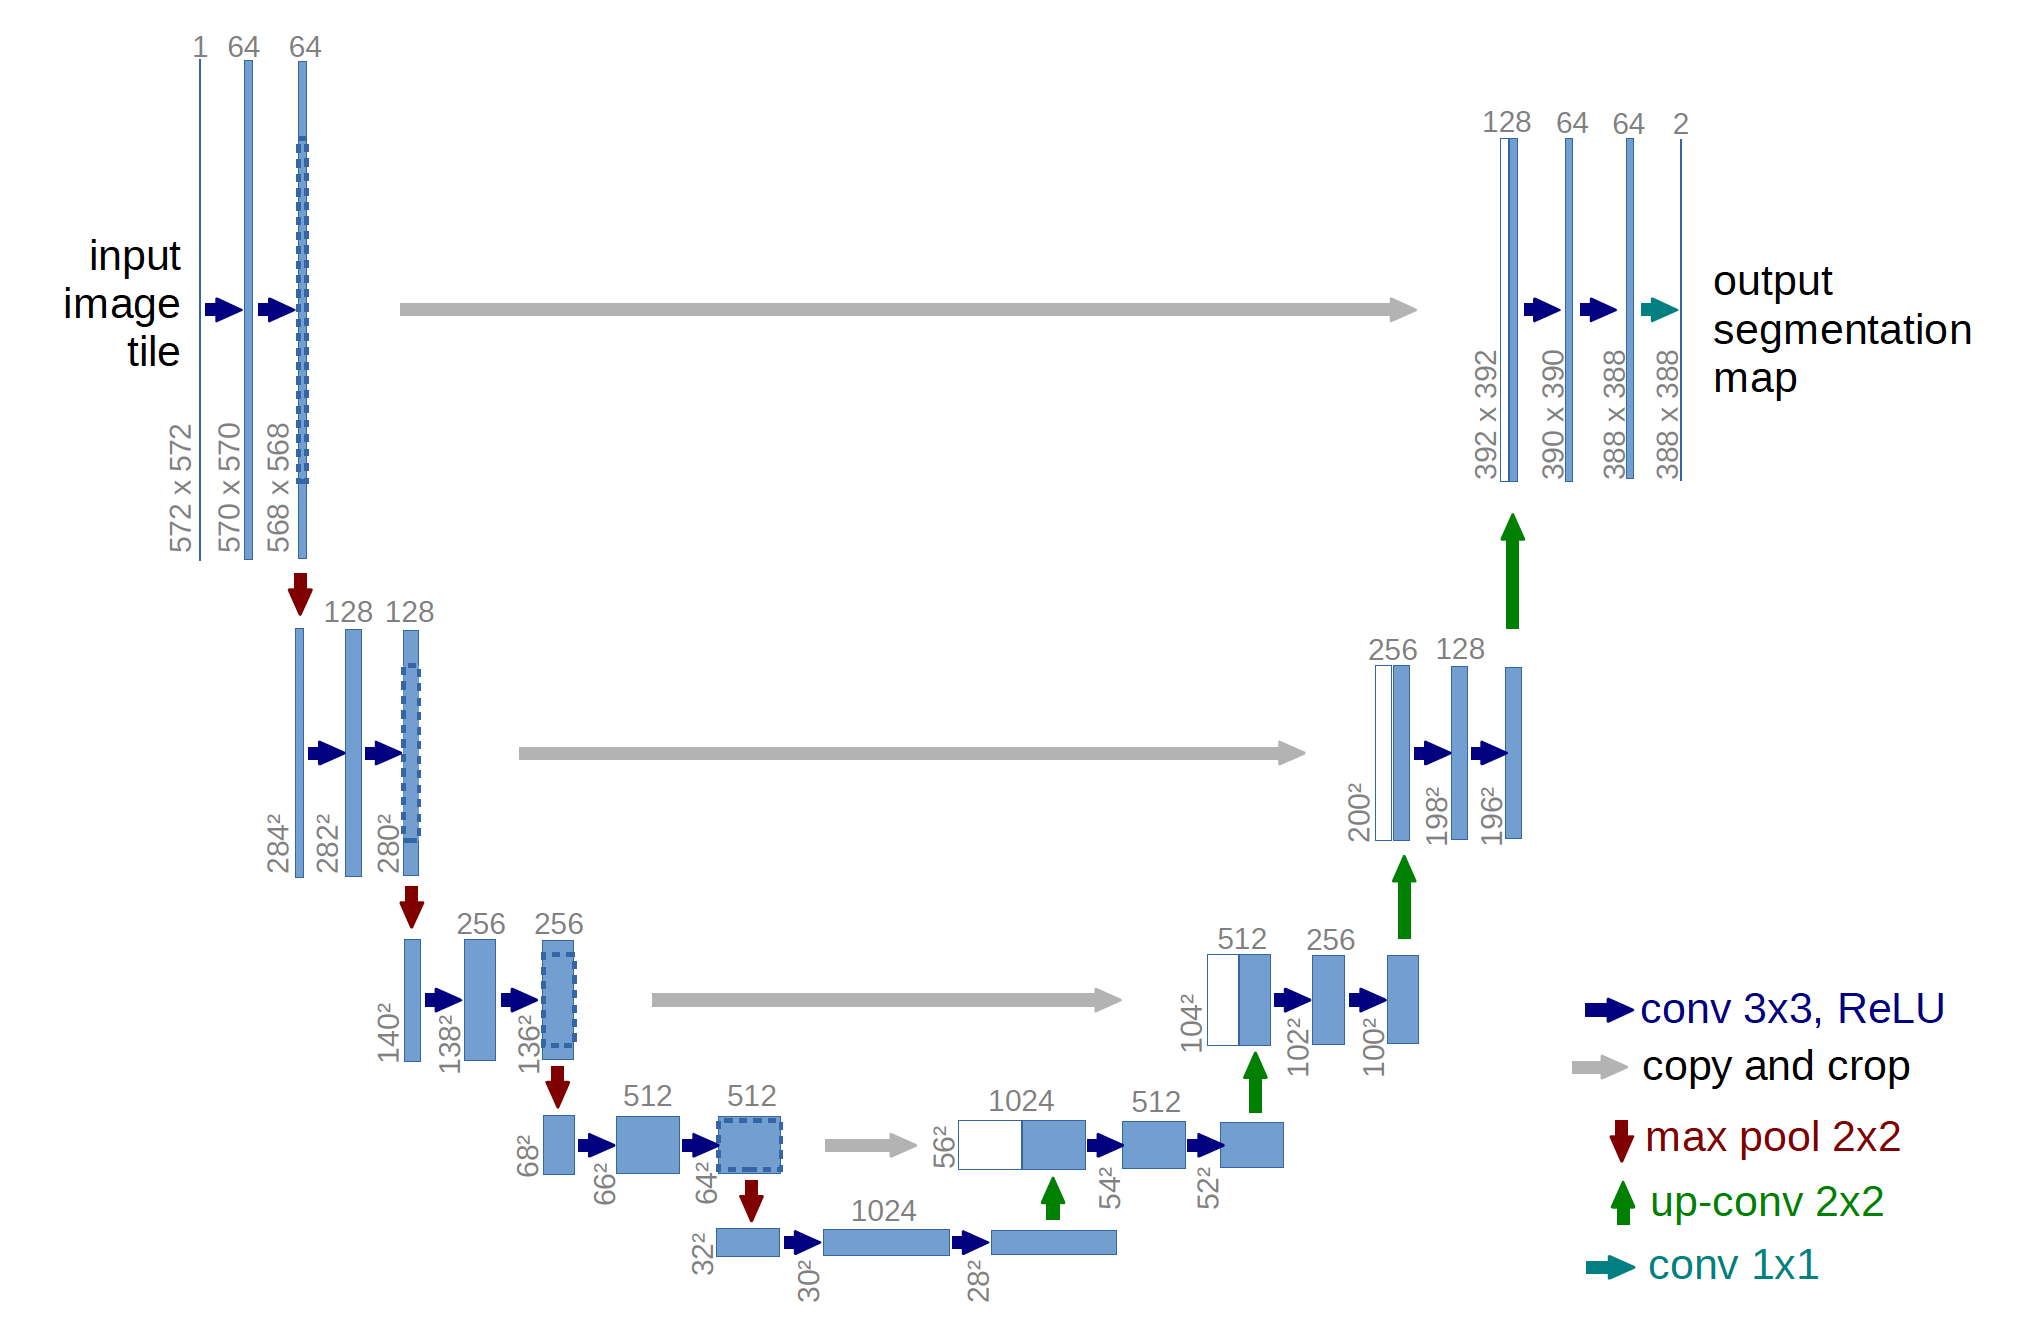
\includegraphics[width=0.8\linewidth]{chap2_Unet.png}
\end{center}
\caption{U-net架构\cite{ronneberger2015u}(最低分辨率为$32\times32$像素图片的示例)。每个蓝色矩形框对应于多通道特征图。通道数显示在矩形框顶部。 特征图的尺寸在的矩形框左下边缘。白色矩形框表示复制的特征图。箭头表示不同的操作。}
\label{fig:chap2_Unet}
\end{figure}

\textbf{空洞卷积}~
Fisher Yu 等\cite{yu2015multi} 提出了空洞卷积架构,这种结构代替了池化,一方面它可以保持空间分辨率,另外一方面它由于可以扩大感受野因而可以很好地整合上下文信息,见图\ref{fig:dilatedConv1}和\ref{fig:dilatedConv2}

\begin{figure}[h]
\begin{center}
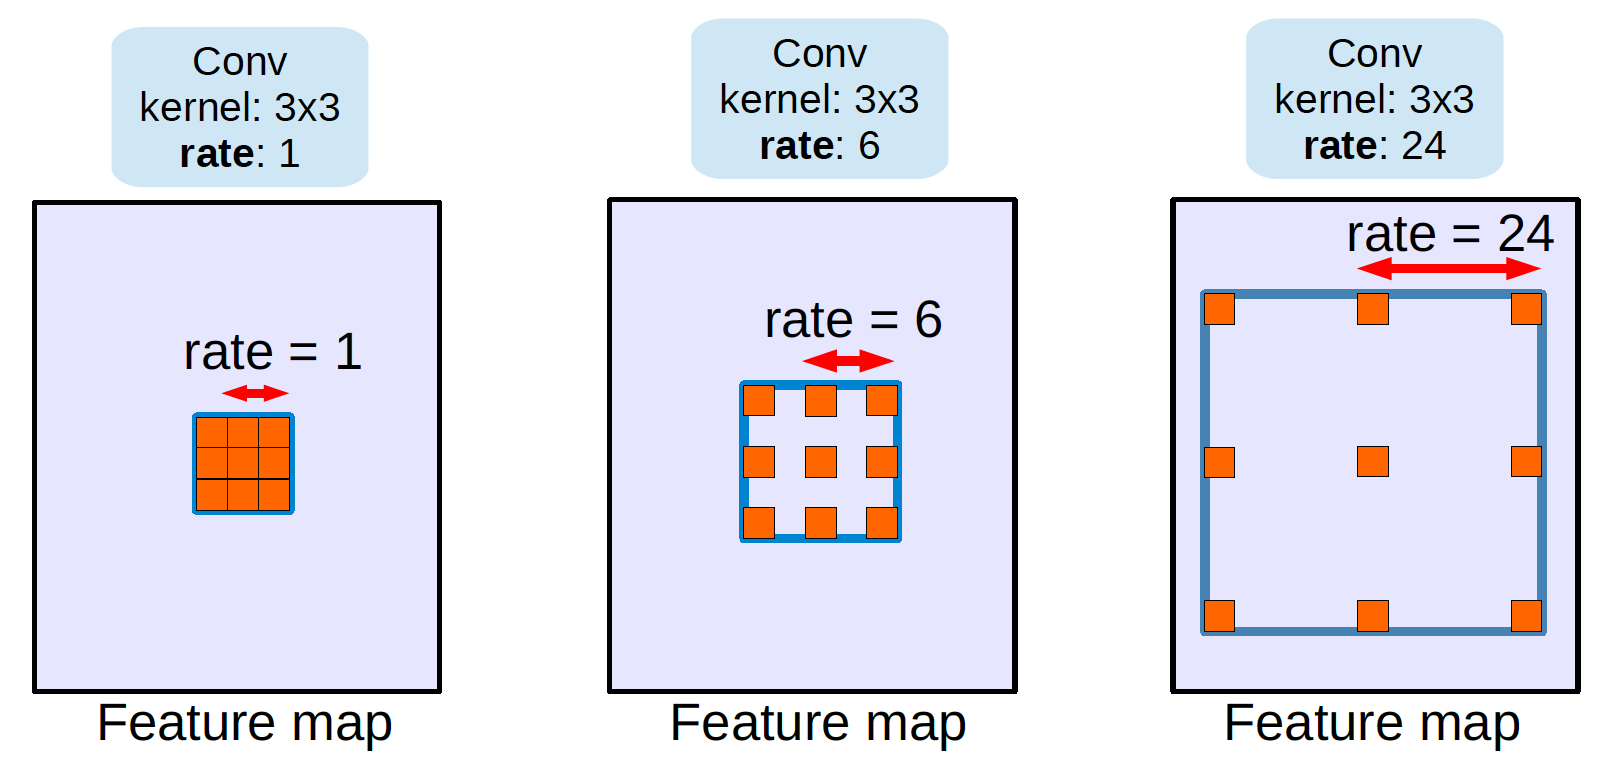
\includegraphics[width=0.7\linewidth]{diConv1.png}
\end{center}
\caption{核大小为 $3\times3$ 和不同步长的空洞卷积\cite{yu2015multi}。 标准卷积对应于步长为1。采用大的步长扩大了模型的感受野,可以在多个尺度上实现对图像编码。}
\label{fig:dilatedConv1}
\end{figure}

\begin{figure}[h]
\begin{center}
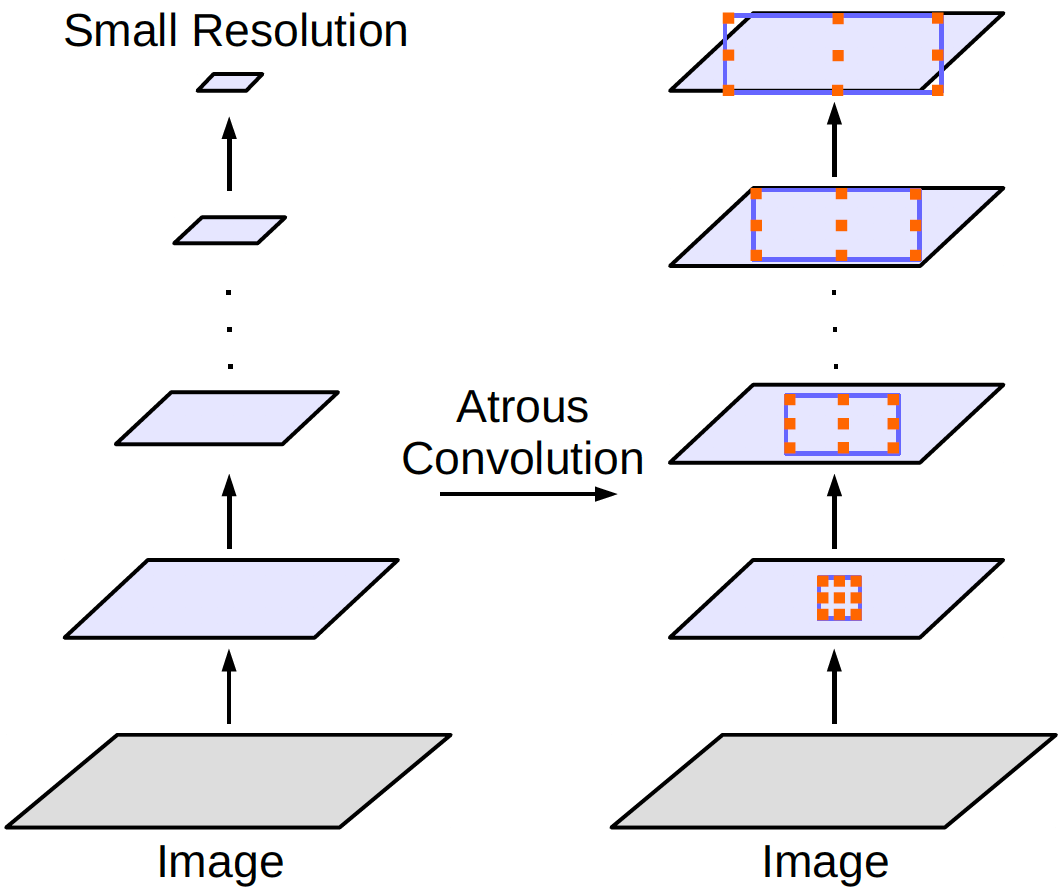
\includegraphics[width=0.5\linewidth]{diConv2.png}
\end{center}
\caption{使用空洞卷积\cite{yu2015multi}进行下采样}
\label{fig:dilatedConv2}
\end{figure}


\textbf{DeepLab系列}
\cite{chen2017deeplab}
同样使用了空洞卷积结构,可以在不增加参数的情况下扩大感受野,保持分辨率,并在此基础上提出了感受野金字塔池化,用来整合多尺度信息。同时在分割后使用全连接条件随机场(fully connected CRF)进行后处理,改善分割结果。并通过两种方式来进行多尺度的处理,一是将原始图像的多种尺度送给网络进行训练,二是通过平行的不同空洞率的空洞卷积层来获得。

\begin{figure}[ht]
\begin{center}
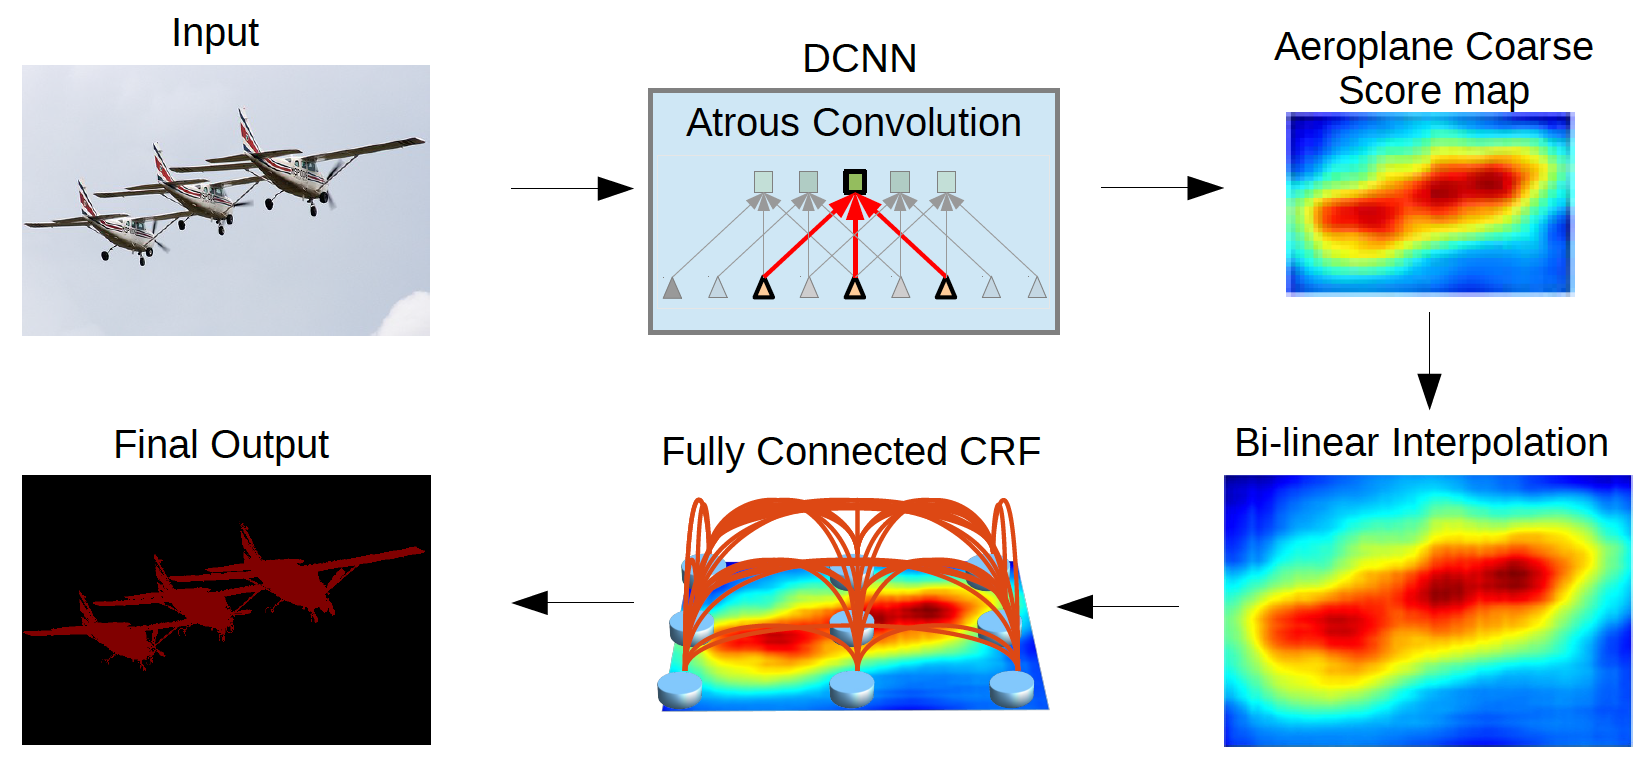
\includegraphics[width=0.8\linewidth]{DeepLab2.png}
\end{center}
\caption{DeepLab模型流程图\cite{chen2017deeplab}。 完全诸如VGG-16或ResNet-101的深度卷积神经网络卷积方式,使用空洞卷积来下。采样双线性插值将特征映射放大到原始图像分辨率。 然后采用完全连接的CRF用于细化分割结果并更好地展现对象的边界。}
\label{fig:DeepLab2}
\end{figure}

\begin{figure}[ht]
\begin{center}
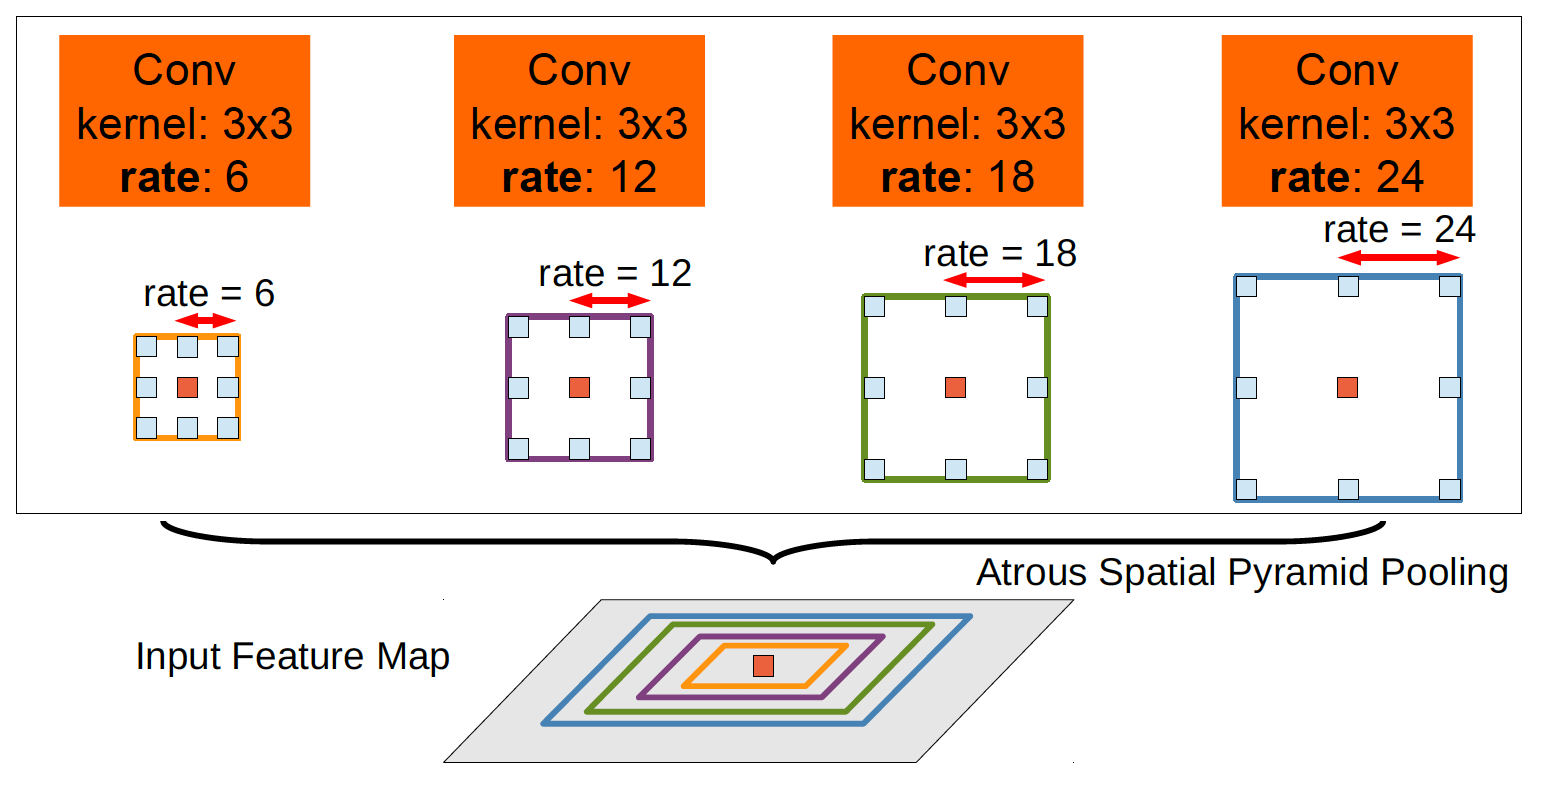
\includegraphics[width=0.8\linewidth]{DeepLab1.png}
\end{center}
\caption{空洞卷积金字塔池化\cite{chen2017deeplab}。 为对中心橙色像素进行分类,ASPP利用了多尺度并行的空洞卷积操作。}
\label{fig:DeepLab1}
\end{figure}

因为空洞卷积方法应用于语义分割也是有缺点的,即使用了大分辨率的特征图,因此计算代价大,并且需要大量的内存,于是Guosheng Lin等在2017年提出了RefineNet\cite{lin2017refinenet}。RefineNet使用编码器-解码器架构。编码器部分使用RESNET-101。解码器部分具有RefineNet 结构,它将此前解码器的低分辨率特征和编码器部分高分辨率特征进行叠加,见图\ref{fig:RefineNet1}。
\begin{figure}[ht]
\begin{center}
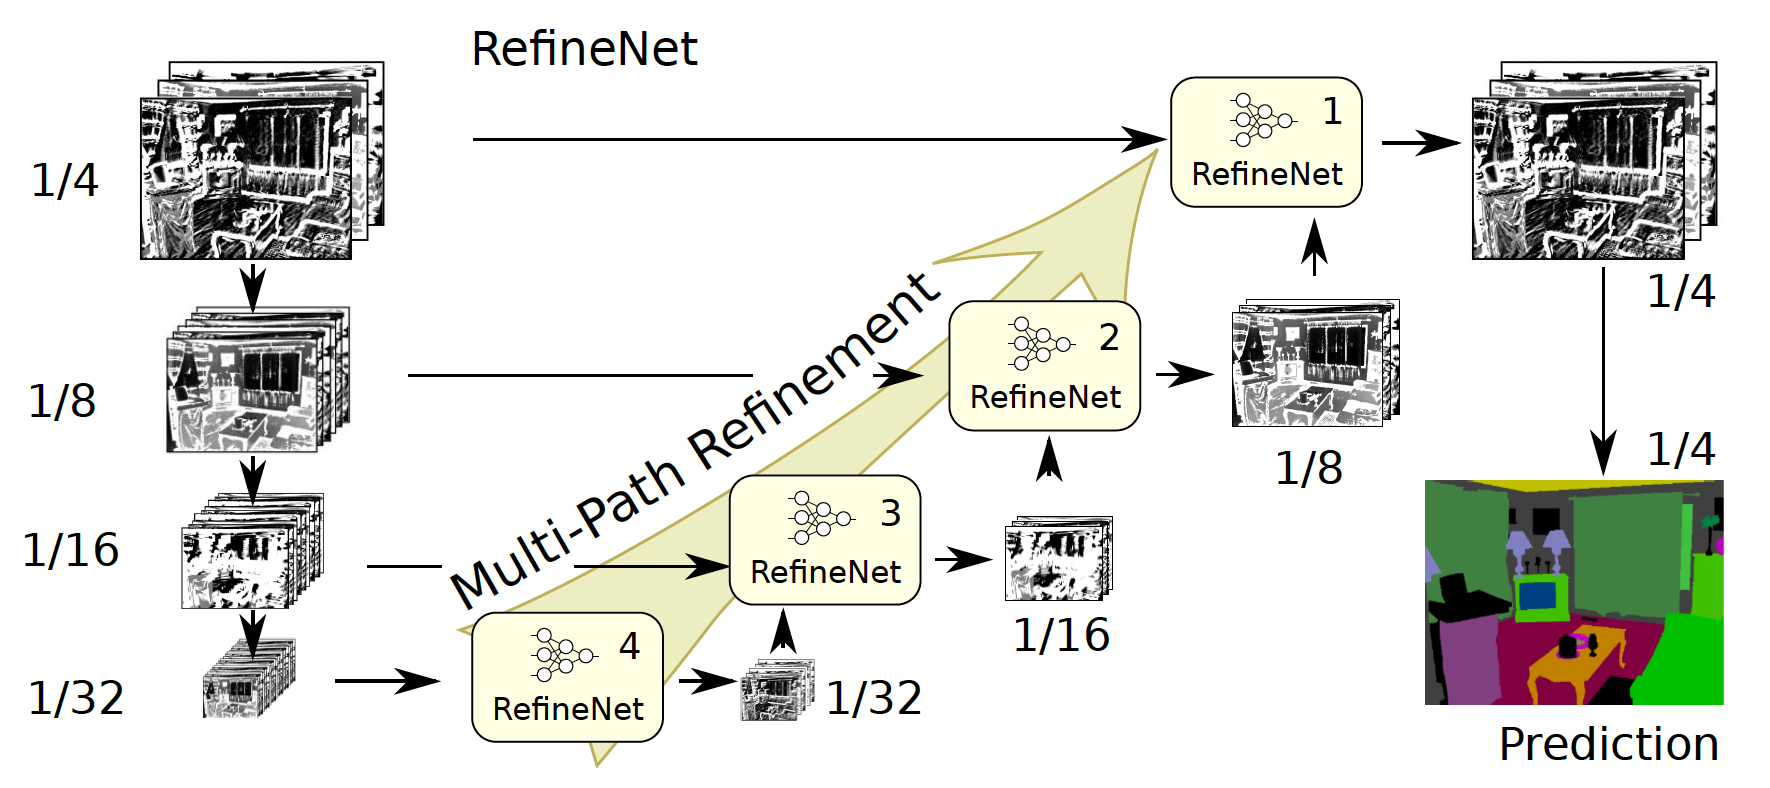
\includegraphics[width=0.8\linewidth]{RefineNet1.png}
\end{center}
\caption{RefineNet架构\cite{lin2017refinenet}。 在卷积的不同阶段利用各种层次的细节,并将它们融合以获得高分辨率的分割图,无需保存或者计算中间过程的特征图。}
\label{fig:RefineNet1}
\end{figure}

\section{弱监督分割相关研究}

由于语义分割训练需要对图像中的每一个像素进行标注,导致标注数据非常耗时,其复杂程度远远超过图像分类、目标检测。想要训练一个分割模型往往需要耗费大量的人力在掩模图像的标注上。为了解决这一问题,人们探究用 图像级别的分类标签、检测标签或者Scribble这样比较容易的标注来训练语义分割模型,这就是弱监督语义分割。通过调研近些年弱监督领域的论文,其基本思想具有下面三个特点:
\begin{enumerate}
\item 大多使用类激活图获取最特别的响应区域,作为最初始的种子类别,然后通过扩张种子区域的方式完成分割。
\item 大多与传统算法相结合。由于深度学习的分割只是看高层语义之间的一致性,没有考虑位置与颜色等低级别一致性,在做相似度度量的时候往往无法满足要求。
\item 流程目前大多还都比较繁琐,一般都需要多次扩充和更新监督信息,进行多轮训练。
\end{enumerate}

在2018年,Yunchao Wei 等\cite{wei2018revisiting} 的主体思路是利用在ImageNet上预训练的分类模型加上不同扩张率的空洞卷积,在图像上得到响应图定位物体,通过阈值分割之后用在类激活图上选择响应较大的区域,将其作为监督来训练网络。其优势在于把空洞卷积使用于分类网络,并且通过改变卷积的扩张率控制热图响应的稀疏程度。

\begin{figure}[ht]
\begin{center}
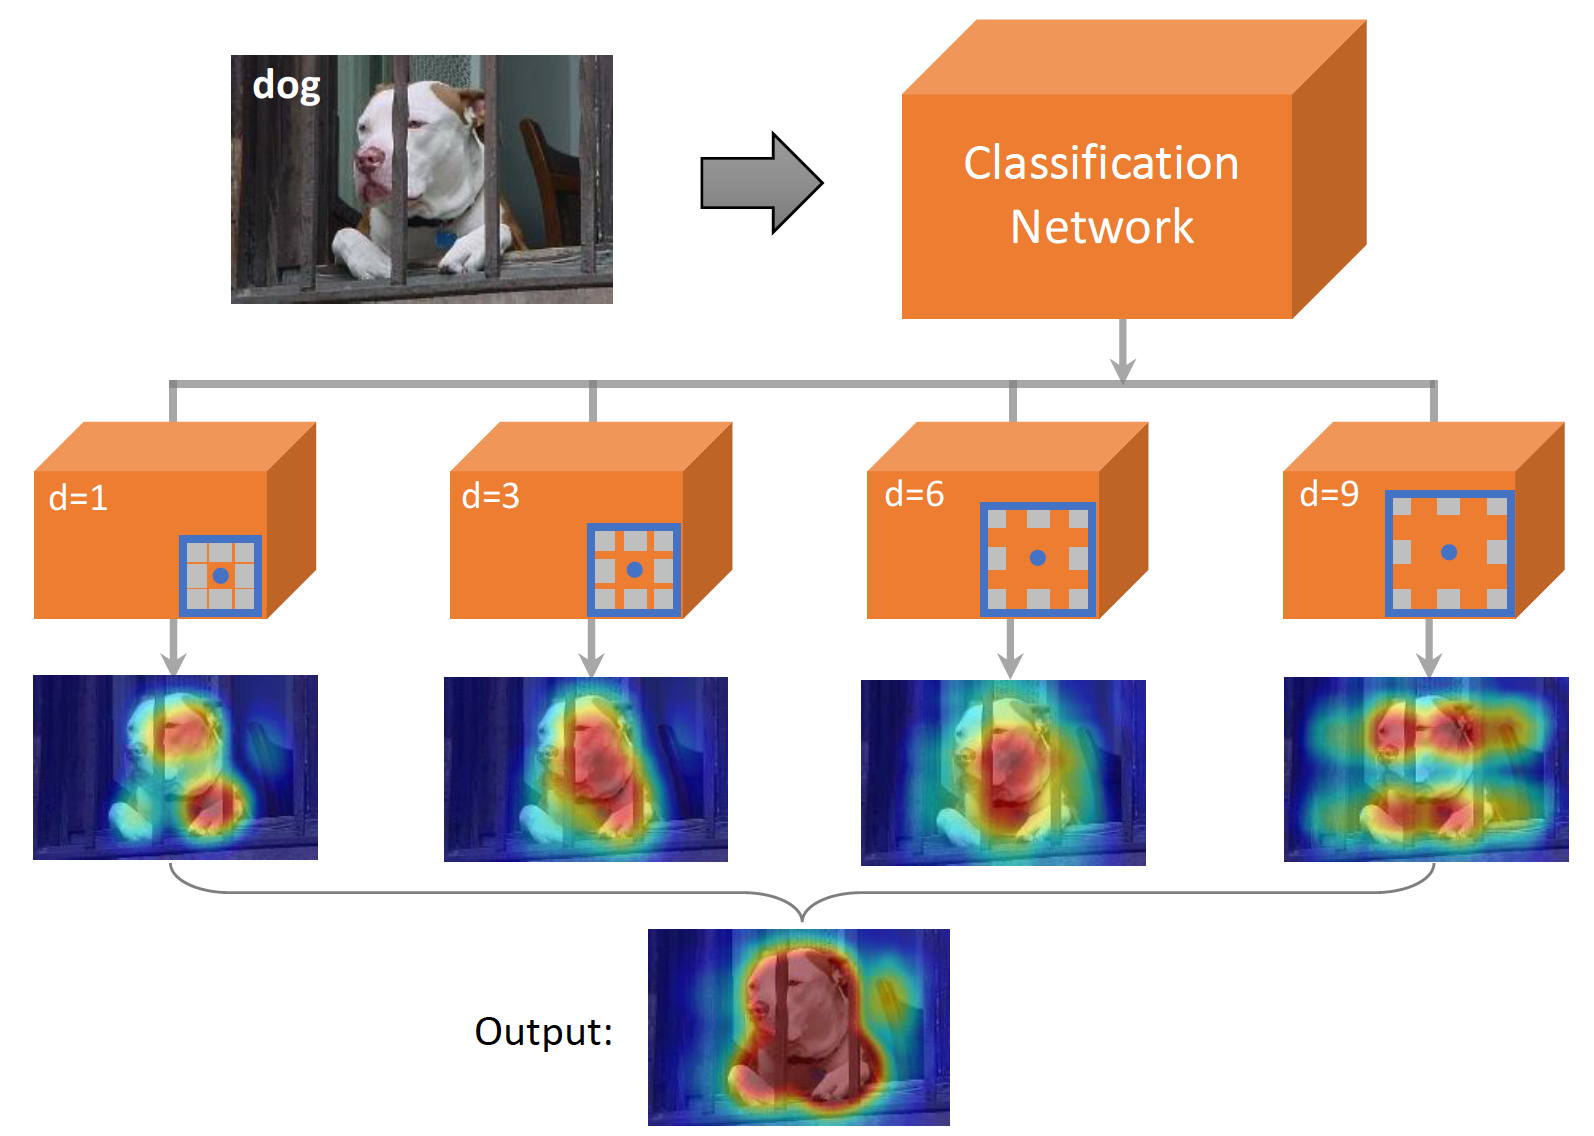
\includegraphics[width=0.6\linewidth]{dilatedConvWeaklySupervised1.png}
\end{center}
\caption{通过多种尺度的空洞卷积生成类激活图\cite{wei2018revisiting}}
\label{fig:dilatedConvWeaklySupervised1}
\end{figure}

\begin{figure}[ht]
\begin{center}
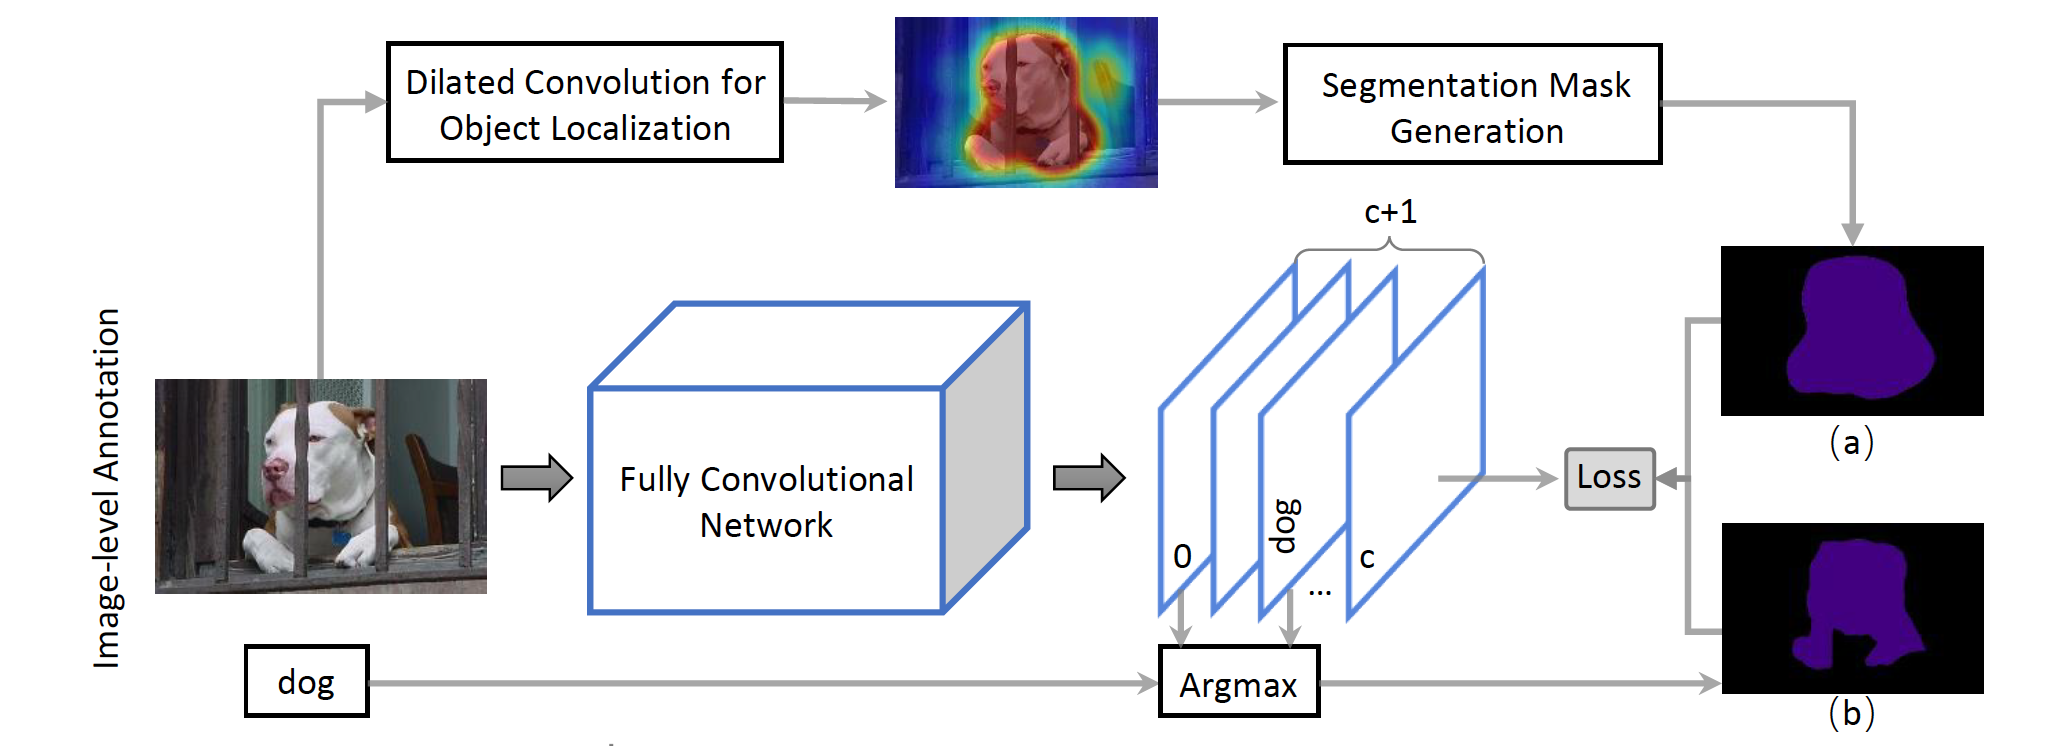
\includegraphics[width=\linewidth]{dilatedConvWeaklySupervised2.png}
\end{center}
\caption{训练流程\cite{wei2018revisiting}。使用生成的类激活图作为监督。}
\label{fig:dilatedConvWeaklySupervised2}
\end{figure}

如图\ref{fig:dilatedConvWeaklySupervised1} 中 $d = 1$所示,热图响应的问题在于只能找到一些具有判别性的稀疏区域,而物体的很多特征不明显的区域会被忽略,而用扩张率较大的空洞卷积可以得到较大的响应区域。 采用如下公式把得到的响应加权以得到较好的预测结果。
\begin{equation}
H=H_{0}+\frac{1}{n_{d}} \sum_{i=1}^{n_{d}} H_{i}
\end{equation}
$H_{0}$代表 $d = 1$的结果,$n_d$就是不同扩张率卷积的个数。整个网络做弱监督的训练流程就如图\ref{fig:dilatedConvWeaklySupervised2}所示,使用多扩张率空洞卷积网络从图像级的标注变为粗糙的预测(a),然后把(a)用作分割的监督信息。

同样在2018年,Xiang Wang等\cite{wang2018weakly}也是用分类网络的热图响应作为起始种子,之后采用迭代的方法,训练两个网络:RegionNet 和 PixelNet,令该两个网络的预测交替成为对方的监督标签,多轮迭代之后,两个网络的预测结果都逐步提升,测试时就使用训练好的PixelNet做单次预测。

由于起始种子部分仅仅覆盖了的很小局部,所以训练出来的RegionNet的结果也会遗漏很多区域,直接做监督效果不好。所以加入了Saliency-guided Refinement模块,相当于使用显著性检测的结果扩充RegionNet的输出。 区别于逆向擦除方法,这里不断更新RegionNet的结果来当做PixelNet的监督,使得预测错误的标签有不断修正的可能。传统的方法不断的扩充标签区域当做训练样本,使得在某一步被误分类的区域一直保留在标签集中误导训练结果。
\begin{figure}[ht]
\begin{center}
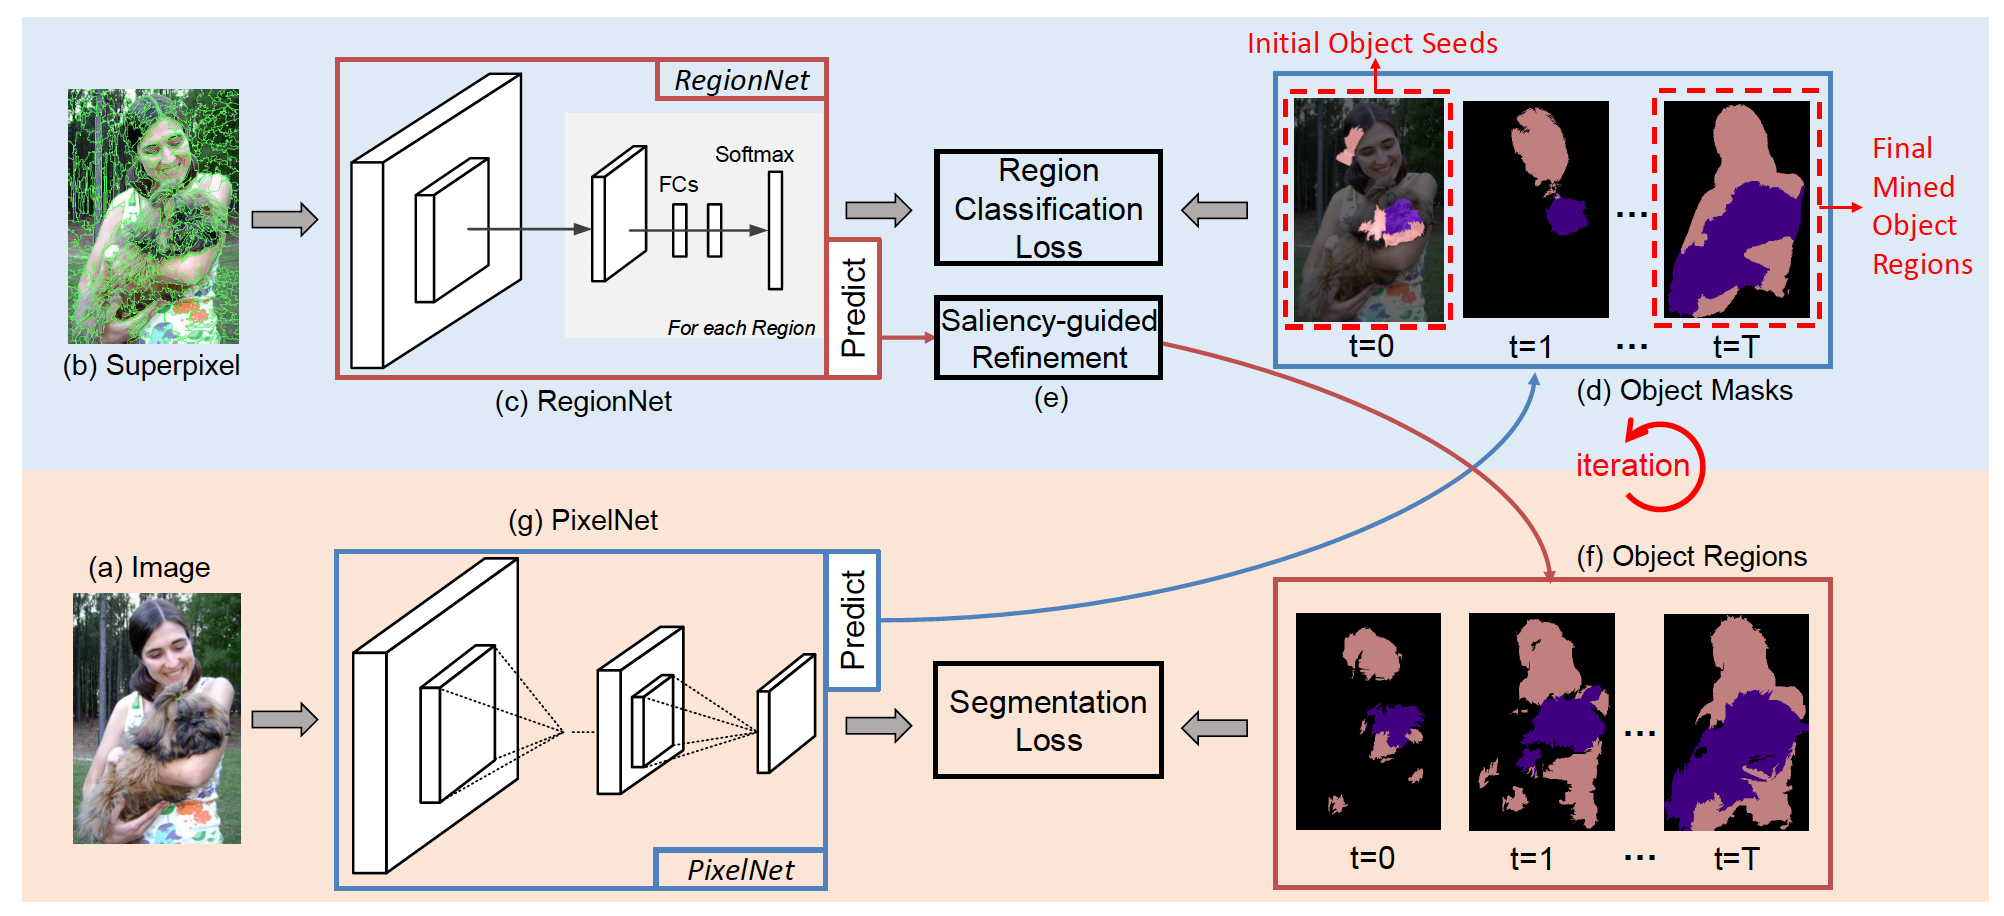
\includegraphics[width=\linewidth]{IterativelyMiningWL.png}
\end{center}
\caption{使用两个网络交替作为监督训练\cite{wang2018weakly}。对于(a),先用传统算法划分成小的区域得到(b) 超像素,然后使用预训练的分类模型在(b)上得出类激活图,取响应最高的部分作为起始种子,如右上角$t = 0$的情况。然后以得到的初始种子点作为监督训练RegionNet。把RegionNet的结果当做监督训练PixelNet。把PixelNet的预测结果当做监督训练RegionNet。不断地重复上述过程。}
\label{fig:IterativelyMiningWL}
\end{figure}


同样在2018年,Zilong Huang等\cite{huang2018weakly}的主体思路是利用预训练好的分类网络在图像上得到类激活图,用最据判别性的小区域作为起始的种子点, 然后改进传统的区域生长方法,使得被标记的区域从起始的小区域不断扩充,在训练过程中逐步得到更多的监督区域。与\cite{wang2018weakly}不同的是起始区域的扩张方法和训练所用的代价函数。这篇文章中,训练的代价函数分为种子代价和边界代价,分别用于约束区域与边界。扩张方法利用的是网络输出的结果。在语义特征层面计算像素之间的相似度,在已经有标签区域的相邻像素点计算和各个类别的相似度,相似度大于某一个阈值就把相邻点扩充进预测概率最大的那一个类别。所以,随着训练次数的增多,已标注区域区域会越填越满,提供的监督信息也会越来越多。

但其缺点是,使用区域生长方法得到的监督无法剔除被标错的区域。也就是说如果一开始有扩充错的区域,那么该区域就不会再接下来的训练中被更正。
\begin{figure}[htbp]
\begin{center}
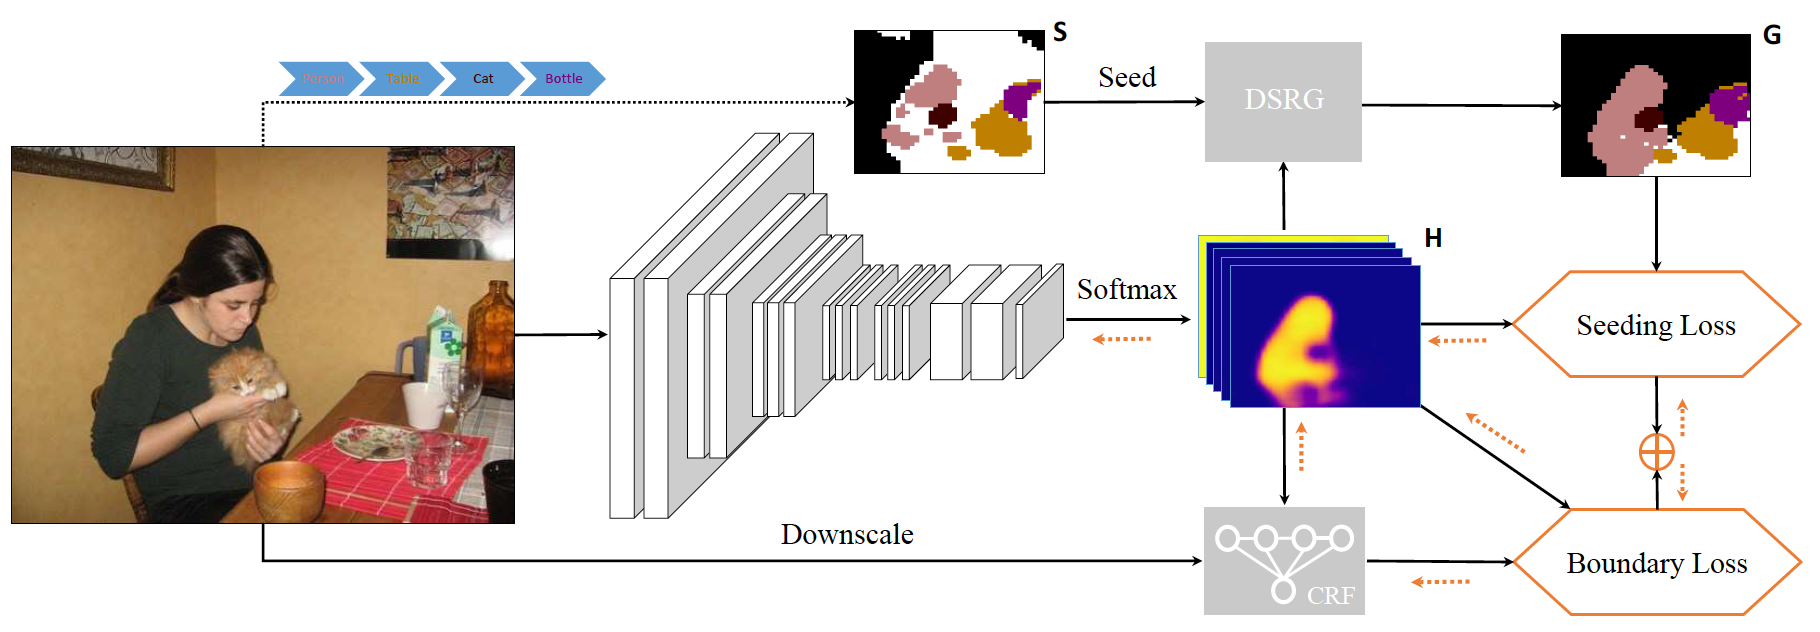
\includegraphics[width=\linewidth]{RegionGrowingWL.png}
\end{center}
\caption{使用类激活图确定种子区域,然后使用区域生长方式扩充区域,同时结合区域代价与边界代价对网络进行训练\cite{huang2018weakly}。}
\label{fig:RegionGrowingWL}
\end{figure}

Yanzhao Zhou等\cite{zhou2018weakly}同样在2018年发表了其关于弱监督下的实例分割方法,据本文作者所知,应该这是第一篇将弱监督用于实例分割任务的工作。其思路非常新颖: 先训练一个网络,使得网络响应的局部极大值可以指示每一个实例物体所在的位置,然后用这些局部极大值的点反向传播信息,逐层向前找到每层网络与那些极大值点相对应的区域,得到峰值响应图 (Peak Response Map), 之后结合峰值响应图以及其提供的边界、位置、类别信息,结合现有的一些传统算法,提出局部的掩模,然后通过非极大抑制 (NMS)得到较为精细的实例分割结果。

由于类激活图的峰值代表图片中某个类别最据判别性的部分,但是不一定可以代表每一个实例的位置。于是,这篇文章首先训练一个网络使得类激活图的局部峰值可以对应每一个实例的位置,如\ref{fig:PRM1}蓝色区域所示。
\begin{figure}[htbp]
\begin{center}
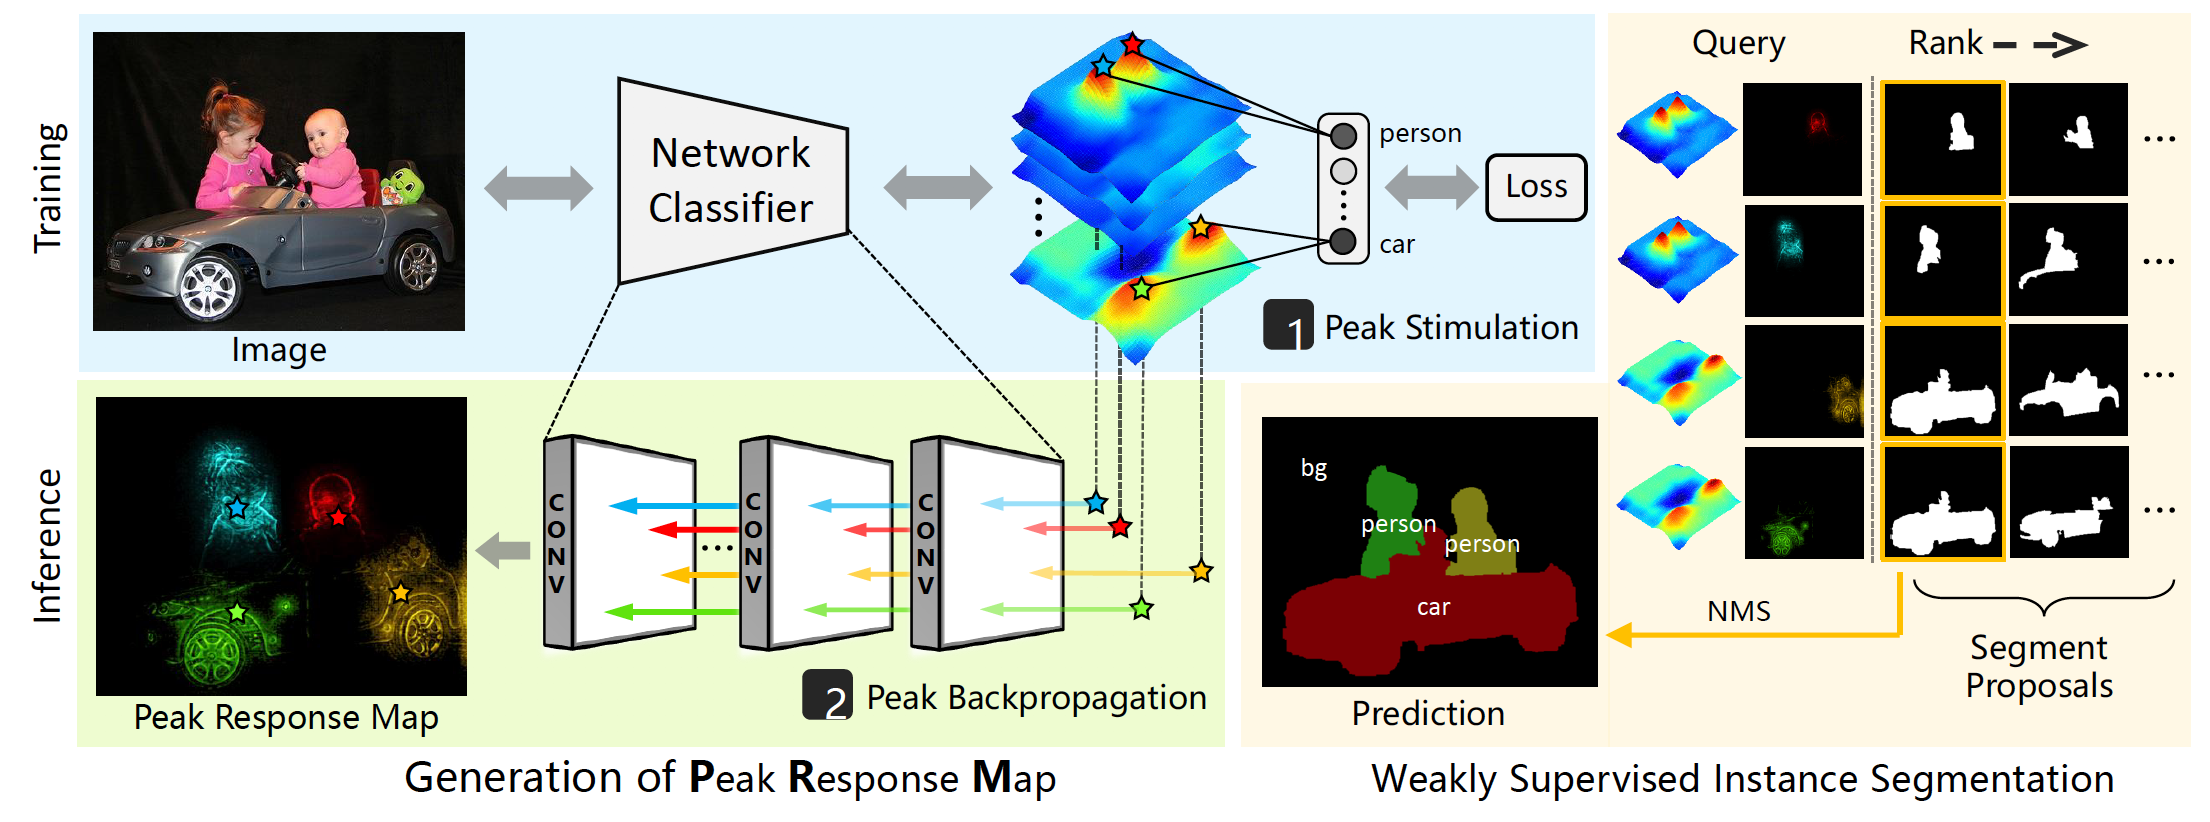
\includegraphics[width=\linewidth]{PRM1.png}
\end{center}
\caption{峰值响应图的生成过程\cite{zhou2018weakly}}
\label{fig:PRM1}
\end{figure}

值得注意的是,在训练时作者先用了一个Dirac函数在类激活图上卷积,目的是只提取峰值区域,这是因为只有峰值的那几个点是想要的有效区域(正样本),其他的大块区域都是并不代表实例的负样本,如果不把峰值区域提取出来,这少数的几个点所提供的正样本的梯度就会淹没在大量的负样本之中。在推理的时候,作者先用训练好的网络找到代表每一个实例位置的峰值点,然后通过反向传播计算这些峰值点来自于前一层每个点的概率,这样一层一层向前推算,就得到第一层的峰值响应图, 如图\ref{fig:PRM2}所示。 得到了峰值响应图之后,利用各种传统算法预测出来局部掩模,最后利用峰值响应图的信息和类别信息进行筛选,然后再这些掩模之中进行非极大抑制 (NMS) 即可。

\begin{figure}[htbp]
\begin{center}
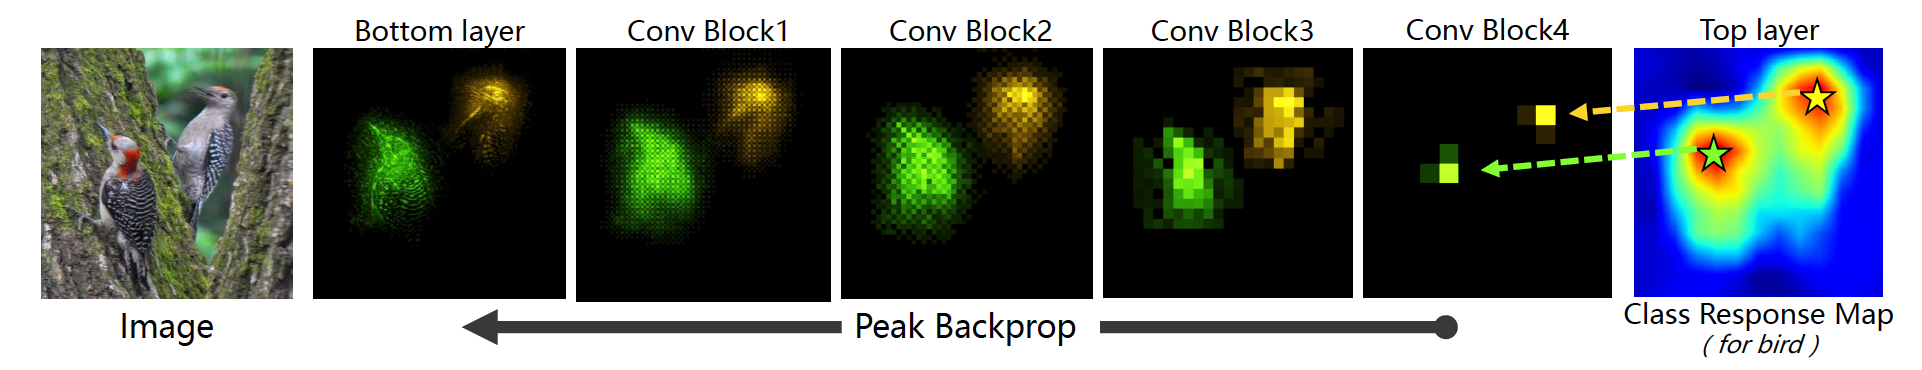
\includegraphics[width=\linewidth]{PRM2.png}
\end{center}
\caption{峰值响应反向传播过程\cite{zhou2018weakly}}
\label{fig:PRM2}
\end{figure}

近几年来,还有一些弱监督分割的方法。例如,通过涂鸦\cite {lin2016scribblesup, xu2015learning}和物体边界框\cite {dai2015boxsup}对图像进分割。然而,这些方法仍然需要大量的人力。一些研究使用图模型来推断区域的标签\cite {zhang2015weakly, lai2016saliency},但他们的对物体的检测能力仍然难以尽如人意。有些方法\cite {papandreou2015weakly, bearman2016s, wei2016learning}试图通过使用可以对位置提出猜测的探测器来定位对象\cite {arbelaez2014multiscale, cheng2014bing}。然而,由于探测器使用边界框标注或对象边界标注进行训练,因此仍需要大量人力。

相反,在本文的工作中,基于类激活图\cite{zhou2018weakly,huang2018weakly}的思想,使用标准分类网络来生成具有卷积响应的类感知激活图,然后结合基于超像素上所建立的图模型,再通过显著性传播实现分割,在此框架中,白癜风区域的边界得到很好的保留。
\section{超像素分割}\label{sec:SLIC}
\subsection{方法原理}
Achanta等\cite{achanta2012slic}提出了一种简单而优雅的迭代聚类算法 (SLIC),用于将彩色图像分割成超像素。该方法的主要思想便是把一些具有相似特性的像素“聚合”起来,形成一个更具有代表性的大“元素”。而这个新的元素,将作为其他图像处理算法的基本单位。将超像素分割用于白癜风分割任务有三个好处:
\begin{enumerate}
\item 大大降低了维度。使用超像素作为后续算法的输入,可以很大程度上减少后续算法的计算量,提高速度。
\item 可以剔除一些异常像素点。由于在白癜风分割的任务中,图片没有经过精细的校准和增强,且拍摄物体多样,因此,对于噪声或者较小区域的异常点可以通过超像素来剔除。
\item 保留较完整准确的皮损边界。经过实验发现,超像素对皮损边界非常的敏感,因此本文利用这一点,将超像素分割作为弱监督分割方法的预处理。
\end{enumerate}

但是由于输入图像的大小差别很大,如何确定初始种子点数目成为了一个难点,如果初始化种子点数目过多,则既没有办法降低数据维度,也没有达到剔除一些异常像素点的目的;如果初始化种子点数目过少,则没有办法很精确的捕捉皮损边界,这样对之后的弱监督分割方法的效果会产生影响。因此,基于原方法,本文通过自适应地调整超像素的数量,来满足预处理的要求:
\begin{equation}
\label{eq:Nc}
N_{c}=\left(\frac{W}{\rho}-1\right)\left(\frac{H}{\rho}-1\right)
\end{equation}
其中,$N_c$为聚类种子点个数,$W$与$H$分别为图像的宽度和高度,ρ此处定义为种子点密度,取值范围为$[0,min⁡(W,H)]$,实验中取为$20$,可以根据需要设置$\rho$的值。$\rho$越大,种子点越密集,后期得到的每个聚类中心面积就越小,分割越细致,但过大的密度会增加计算量,并且容易受到图像噪声的干扰,导致图像分割效果变差。

\begin{figure}[htbp]
\begin{center}

\includegraphics[height=1.5cm]{chap3_superpixelflow.png}
\end{center}
\caption{超像素分割实验流程图}
\label{fig:chap3_superpixelflow}
\end{figure}

\textbf{图像获取}:可使用手机、相机、专业医疗设备对患处拍摄图片,皮肤应占据照片的主体部分,但仍可包含部分背景、衣物、毛发等无关的区域,拍摄时应尽量选择光线较为柔和的环境。在实验部分的测试图片选用Vit2019中的图片作为测试。

\textbf{图像预处理}:此步骤的目的一是为了去除噪声,二是平滑毛发区域中的锐利边缘,避免聚类中心分割时产生过多的不规则形状以及孔洞。对图像使用了高斯模糊和中值滤波来去除噪声。

\textbf{超像素分割}:此部分将有相似特性的像素聚合起来形成超像素。具体算法流程见算法2。
\begin{table}[htbp]
  \centering
    \begin{tabular}{l}
    \toprule
    \textbf{算法2}  改进的超像素分割算法流程\\
    \midrule
    \multicolumn{1}{p{36em}}{1. 将输入RGB图像转换到Lab颜色空间} \\
    2. 根据输入图像尺寸初始化聚类种子点个数,见公式(\ref{eq:Nc})\\
    \multicolumn{1}{p{36em}}{3. 以$\rho$为步长,初始化种子点,记为$\mathrm{C}_{\mathrm{k}}=\left[l_{k}, a_{k}, b_{k}, x_{k}, y_{k}\right], \quad k=1,2, \dots, N_{c}$, 其中$l_{k}, a_{k}, b_{k}$ 分别为图像在Lab空间下位置坐标为$\left(x_{k}, y_{k}\right)$处所对应像素点的L,a,b分量}\\
    \multicolumn{1}{p{36em}}{4. 在以种子点为中心,3×3为大小的领域内,将种子点移动到Lab模型中L通道梯度最小的位置,以防其落到图像边缘上或者噪声处,对后面的聚类过程产生影响。}\\
    5. \textbf{聚类}\\
    \multicolumn{1}{p{36em}}{ \hspace{2em} 5-1. 初始化每一个像素点i的标签数组$l(i)=-1$,距离数组$d(i)=\infty$,初始化最大迭代次数$N_{iter}$} \\
    \hspace{2em}5-2. 以$C_k$为中心,$2\rho \times 2\rho$大小的区域内,计算像素$i$与$C_k$的距离$D$ \\
    \hspace{2em}5-3. 若${D}<{d}({i})$,则令$d(i)=D,l(i)=k$ \\
    \hspace{2em}5-4. 判断是否遍历完所有聚类中心,若是,则继续;否则返回步骤 5-1 \\
     \hspace{2em}5-5. 更新所有聚类中心\\
     \hspace{2em}5-6. 判断是否达到最大迭代次数$N_{iter}$,若是,则结束;否则,返回步骤5-2\\
    6. 增强图像的连通性,最终生成$n$个像素聚类\\
     \bottomrule
    \end{tabular}%
\end{table}%

其中,将像素$i$与像素$j$之间的距离$D$定义为空间距离与颜色距离的加权和:
\begin{subequations}
\begin{align}
\mathrm{D}_{\mathrm{s}}&=\sqrt{\left(x_{i}-x_{j}\right)^{2}+\left(y_{i}-y_{j}\right)^{2}}\\ \vspace{1em}
\mathrm{D}_{\mathrm{c}}&=\sqrt{\left(l_{i}-l_{j}\right)^{2}+\left(a_{i}-a_{j}\right)^{2}+\left(b_{i}-b_{j}\right)^{2}}\\
\mathrm{D}&=\sqrt{\left(\frac{D_{s}}{C_{s}}\right)^{2}+\left(\frac{D_{c}}{C_{c}}\right)^{2}}
\end{align}
\label{eq:D}
\end{subequations}

其中$C_s,C_c$ 分别为空间距离与颜色距离的归一化常项。

\subsection{实验结果与分析}
经过如图\ref{fig:chap3_superpixelflow}所示流程,我们至此,即可得到分割好的$n$个图像的子区域,其中$n$等于算法2步骤6中聚类的个数,如图\ref{fig:chap3_SLICresults1}所示,由蓝色线所形成的每个最小封闭区域即为一个聚类中心。然后我们通过人为施加阈值的方式对白癜风皮损区域进行分割,得到图\ref{fig:chap3_SLICresults1}.c。

此处令公式(\ref{eq:D})中的$C_s=25,C_c=\rho$. 在使用过程中,$C_c$的取值范围可取$[1,40]$之间,该值越大,则$D_s$在距离度量中所占权重越小,则后期所得聚类中心形状越不规则,呈长条状,即难以保证空间的相关性,但对物体边缘较为灵敏,贴合度较高,容易收到噪声的干扰;反之,该值越小,则$D_s$在距离度量中所占权重越大,则后期所得聚类中心形状越规则,类似方块状,不易受到噪声的干扰,但对图像边缘较不敏感。实验中取最大迭代次数为10,可达到效果与计算代价的平衡。

\begin{figure}[htbp]
\begin{center}
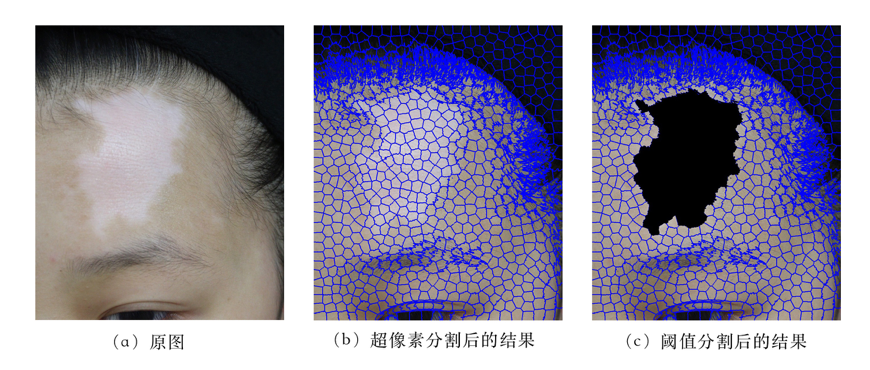
\includegraphics[width=0.9\linewidth]{chap3_SLICresult1.png}
\end{center}
\vspace{-1em}
\caption{超像素分割流程对照结果图}
\label{fig:chap3_SLICresults1}
\end{figure}

\begin{figure}[htbp]
\begin{center}
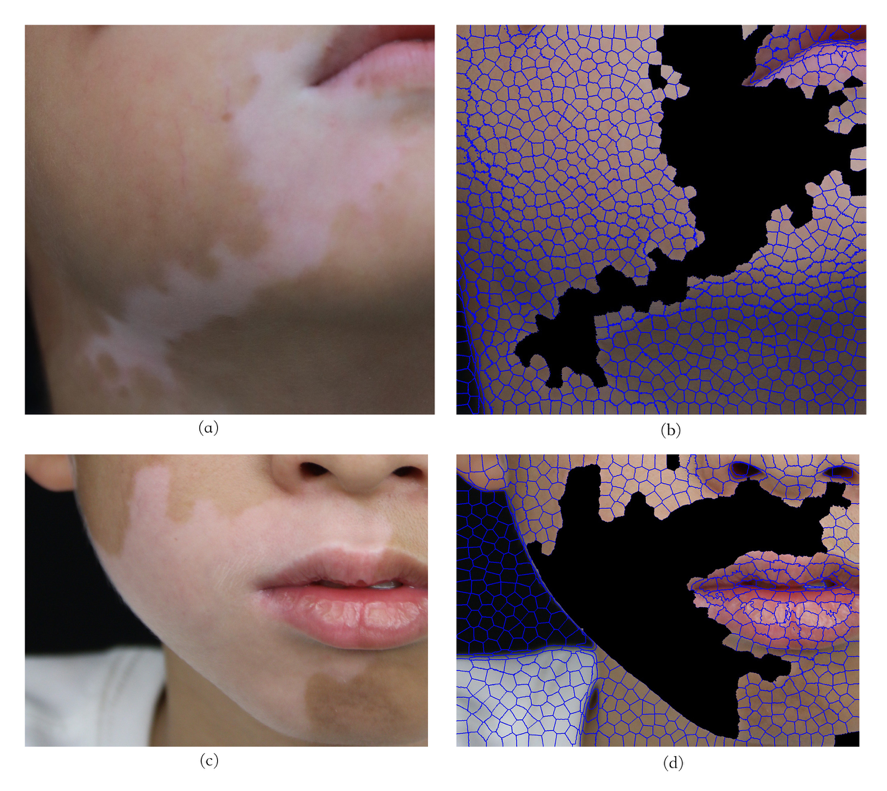
\includegraphics[width=0.6\linewidth]{chap3_SLICresult2.png}
\end{center}
\vspace{-1em}
\caption{超像素分割结果图。(a)(c)表示原图,(b)(d)表示超像素分割后的结果图。}
\label{fig:chap3_SLICresults2}
\end{figure}

通过实验可以发现,将超像素分割方法应用于白癜风图像的预处理有以下的优点:
\begin{enumerate}
\item 操作简单方便,对硬件设备没有特殊要求。
\item 可适应白斑边界模糊且图像对比度低的情况,如图~\ref{fig:chap3_SLICresults2}.a。
\item 由于引入超像素作为一块区域的代表,即便处理高分辨率图像仍可做到快速分割。算法速度可参见表\ref{table:SLICresults}
\item 分割图像不易产生空洞,不依赖于后期的形态学处理。
\end{enumerate}

\begin{table}[]
\centering
\caption{SLIC算法性能测试结果}
\begin{tabular}{cccc}
\toprule
测试图片 & 图片大小         & 运行速度(秒) & IOU  \\ \midrule
  图\ref{fig:chap3_SLICresults1}.a   & 850 × 1011   & 5.6     & 0.89 \\
    图\ref{fig:chap3_SLICresults2}.a   & 1373 × 1305 & 11.9    & 0.82 \\
    图\ref{fig:chap3_SLICresults2}.c   & 1588 × 1152 & 11.6    & 0.86 \\ \midrule
     \multicolumn{4}{c}{硬件环境:2.3 GHz Intel Core i5}\\
     \bottomrule
\end{tabular}
\label{table:SLICresults}
\end{table}

\section{本章小结}
本章首先介绍了近些年来将深度学习应用于图像分割领域的方法和技术,然后引出了基于强监督方法的缺点,即对数据集有很强的依赖性。然后本章对比了近年来各种弱监督分割方法,分析了其各自的优点和缺点,并将其基本的思想做了总结和归纳,为引出本文的弱监督分割框架进行了铺垫。

关于超像素分割部分,首先介绍了一种广泛用于图像分割领域的一种简单而优雅的迭代聚类算法 (SLIC),我们将其作为执行弱监督分割前的一项预处理步骤,并详细解释了将超像素分割用于白癜风分割任务的三个好处,即大大降低了维度、剔除一些异常像素点、保留较完整准确的皮损边界。然后指出了在经典超像素分割算法中初始种子点数目确定难的问题,并针对提出了改进的方法。最后通过实验,定性的展示了超像素分割的效果,为弱监督分割框架的介绍奠定了基础。


\chapter{强监督分割方法及实现}
\section{引言}
强监督学习是相对于无监督学习、弱监督学习而言。尽管当前的技术已经取得了巨大的成功,但是值得注意的是,其方法非常依赖于大规模数据集的标注。该技术通过学习大量训练样本来构建预测模型,其中每个训练样本都有一个标签标明其真值输出。在图像分割领域,每个训练样本所对应的真值应该是像素语义级标注的,即对于图像中每一个像素所属的类别的信息都需要引入训练过程中。 而缺乏大型数据集使得最先进的强监督方法没有用武之地。本文的目的之一是提供一个大规模的白癜风数据集。希望本文的具有像素级标注的白癜风图像可以促进该视觉领域的研究。

本章首先介绍所提出的数据集,然后采用目前常用的强监督的方法对数据集进行测试。
\section{数据集:Vit2019}
现有的皮肤病图像数据集 \cite {mendoncca2013ph,codella2018skin,sun2016benchmark}包含有限的白癜风图像。为此,本文提出了一个新的临床白癜风数据集 “Vit2019”。据我所知,Vit2019是目前最大的像素级标注的白癜风图像数据集。简而言之,Vit2019包含两个类别的2,000个图像:1000个白癜风图像注释像素级和1000个非白癜风图像。样例见图\ref{fig:chap2_DatasetGragh1}。
\begin{figure}[htbp]
\begin{center}
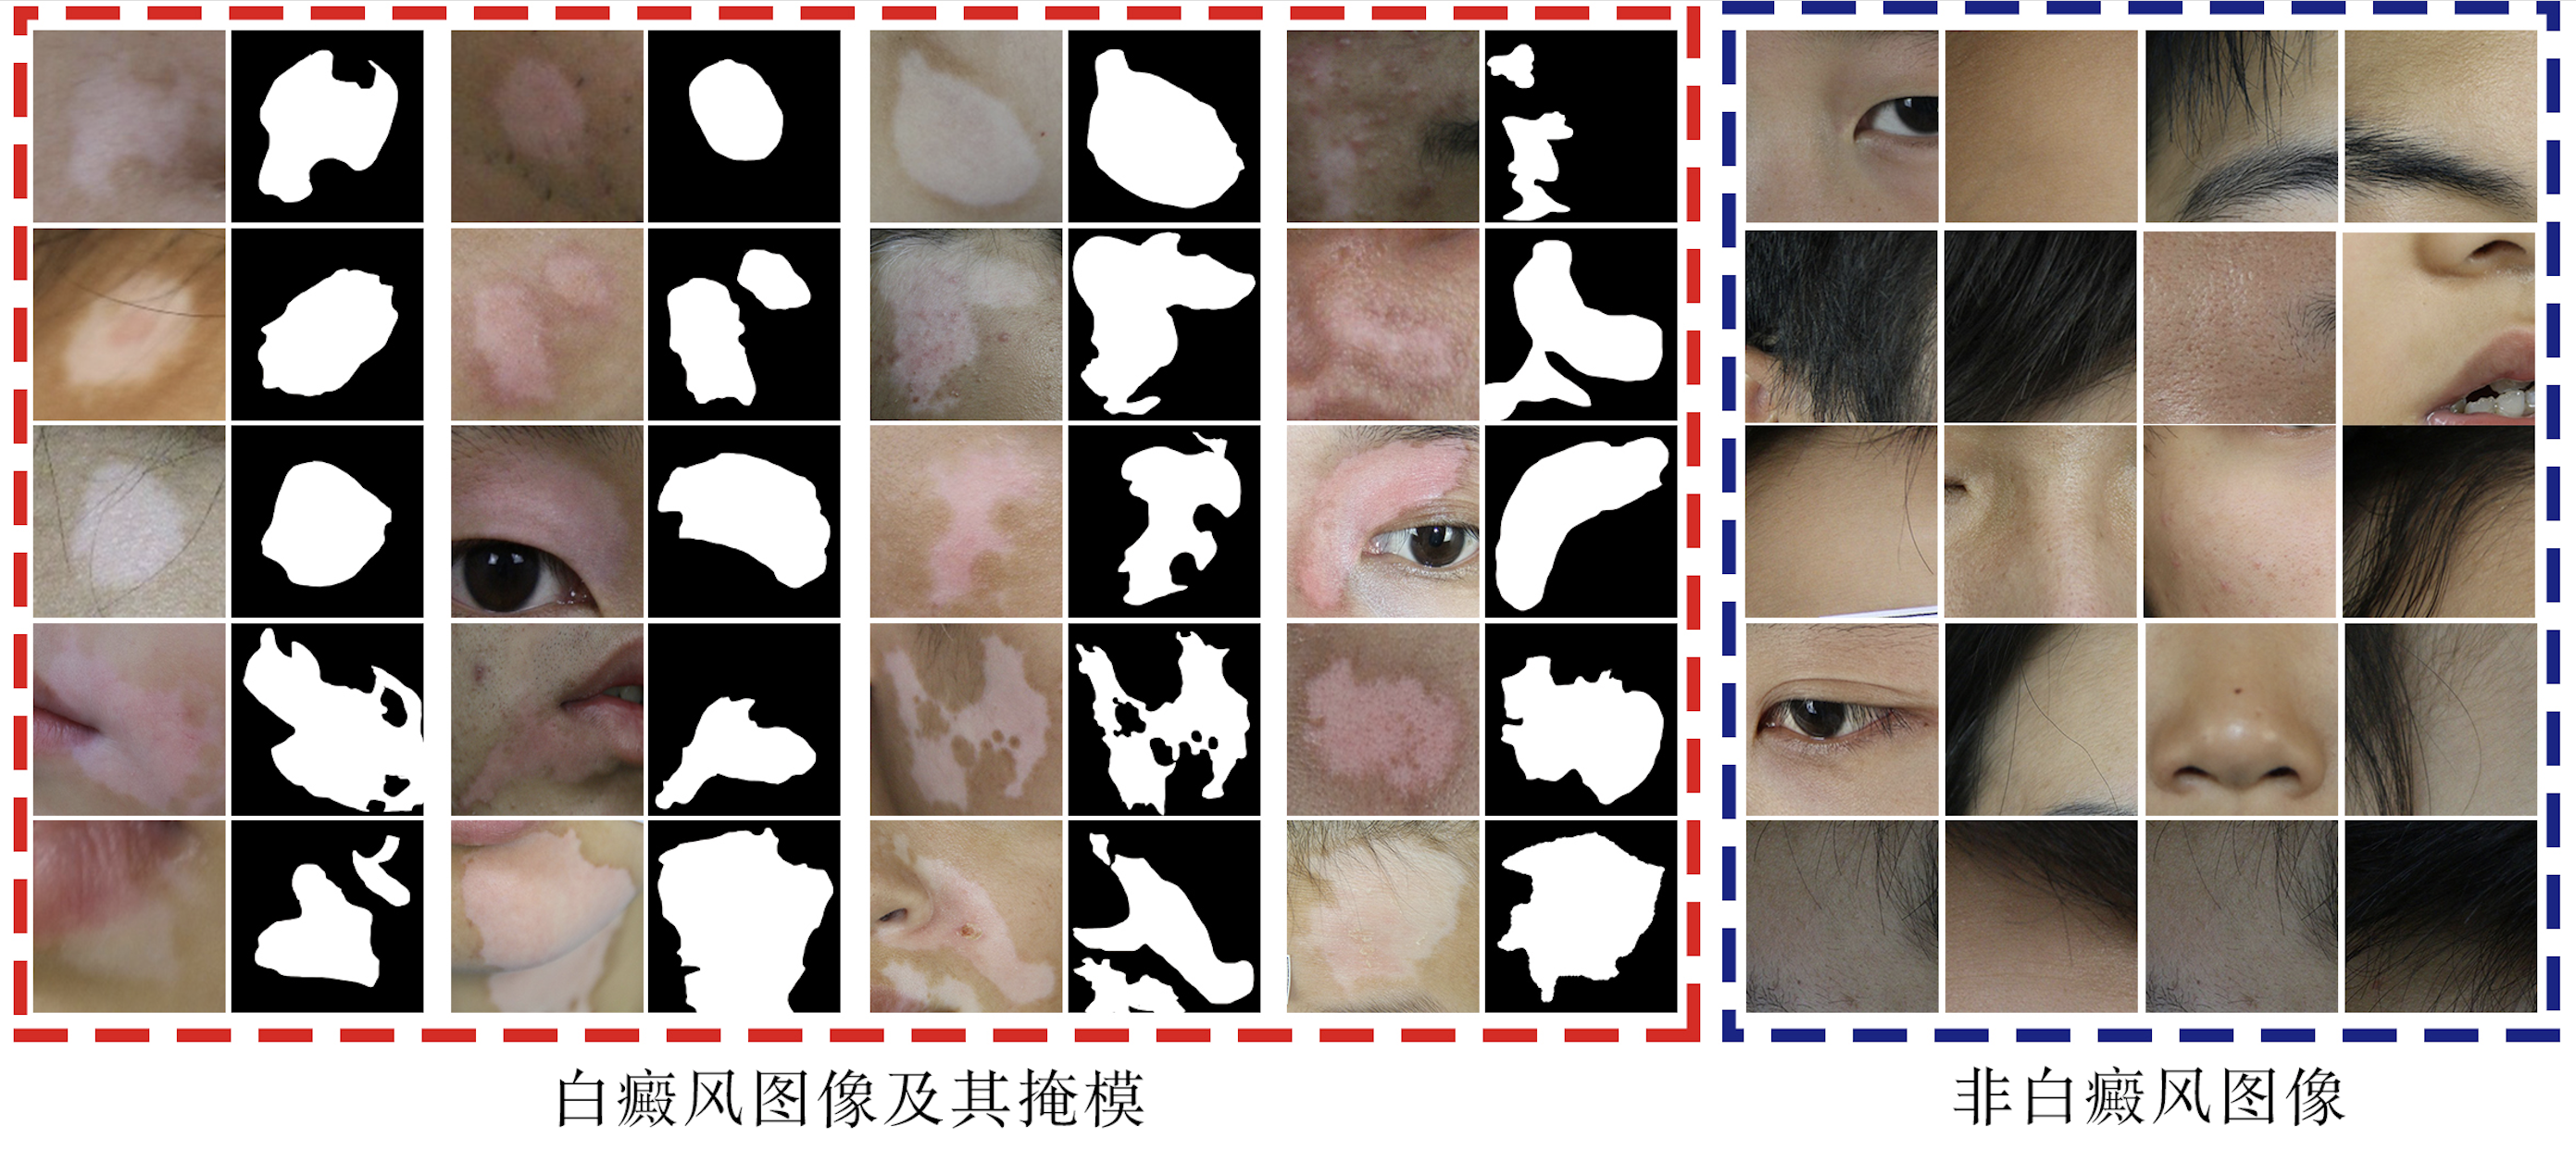
\includegraphics[width=\linewidth]{chap2_DatasetGragh1.png}
\end{center}
\caption{从Vit2019数据集中随机抽取的图像。 (a)白癜风图像。大约70%的图像位于患者的面部和颈部,而其余部分位于身体的其他部位(如躯干,胸部和背部)。 (b)非白癜风图像,其包含健康的皮肤,头发,眼睛,嘴唇,鼻子等。}
\label{fig:chap2_DatasetGragh1}
\end{figure}

\textbf{收集} ~大约800张图像由医院提供,其余图像则从互联网上收集(例如,谷歌图像,DERM101)。其他1,000张非白癜风图像是从没有白癜风病变的区域随机裁剪。

\textbf{标注}~像素级精确地注释白癜风区域是耗时且容易出错的。本文进行了像素级注释,并邀请了两位白癜风专家来审查此数据集,以确保注释质量。

\textbf {多样性}~ 此数据集是在现实世界条件下收集的。它涵盖了不同的环境因素,包括照明和摄像机视角,以及患者的其他属性,如年龄范围(儿童,青少年,老年人),皮肤状况(粗糙,光滑,健康,有其他色素性皮肤病),患病部位(面部,手部,脚部,四肢,头皮),性别,肤色(较深,较浅),不同阶段(早,中,晚)的病变,治疗程度(未经治疗,初始治疗后,经过长时间治疗)以及期限治疗。这使此数据集更加全面和具有挑战性。

\textbf {挑战}~由于数据集中大部分图像来源于临床,因此基于Vit2019中的分割任务在以下意义上具有挑战性:
\begin{enumerate}
\item Vit2019中的图像是在完全不受控制的情况下拍摄的,没有任何图像增强,例如去噪和对比度增强;
\item 图像主要以黄色皮肤为主,白癜风病变颜色浅(呈粉红色,浅黄色),对比度低,有些图像甚至需要专家来标记皮损的边界;
\item 如之前所述,受影响的区域是多样的。一些白癜风区域靠近眉毛或头皮,容易被头发阻挡,而唇部周围的一些白癜风区域易受唇部本身颜色的影响。
\end{enumerate}

\section{方法框架}

此处我们使用经典的``编码器解码器''的强监督分割框架Unet来对Vit2019上的图片进行训练和测试。具体的网络结构请参见第\ref{sec:fullySeg}节。

我们将Vit2019数据集的20\%作为测试集,另一部分作为训练集,在NVIDIA GTX-1080上进行训练,设置为 300个epochs,批量训练的大小设置为16张图片。开发语言选用Python, 深度学习框架使用Pytorch作为基础。Python编译器选用 Python 3.5.


\section{实验结果及分析}

\textbf{衡量指标}~
我们使用IoU这一评价指标来评价分割效果,如公式\ref{eq:IoU}所定义。IoU (Intersection over Union)是一种评估指标,用于衡量特定数据集上对象检测器或者分割的准确性。我们经常看到此评估指标用于图像分割方面的挑战,例如流行的MSCOCO挑战。为了应用Intersection over Union来评估分割效果,我们需要:分割的真值边界(即手工所标记边界,用于指定对象在我们图像中所占区域)和我们模型中预测的区域。我们利用这两组区域,就可以计算IoU。 
\begin{equation}
\label{eq:IoU}
\mathrm{IoU}=\frac{\mathrm {Area\,over\,Overlap}}{\mathrm {Area
\,of\,Union}}
\end{equation}
分子是我们预测的区域面积和真实的区域间的重叠区域。分母是两者区域的联合的区域。

\textbf{定性与定量结果}

如图\ref{fig:UnetResult}展示了U-net的分割效果,测试图片均为从测试集中随机抽取所得。第一列表示输入网络的原图,第二列表示U-net的分割结果,第三列表示手工标记的真值。我们可以发现,对于一些边界明显,对比度强的图片,U-net具有较好的分割能力,但是对于一些对比度差、边界模糊的图片,分割效果不尽如人意。而且可以观察到,U-net的分割结果对于边界细节的保持效果较差。

经过多组测试,得到平均的IoU为78.6\%.

\begin{figure}[htbp]
\begin{center}
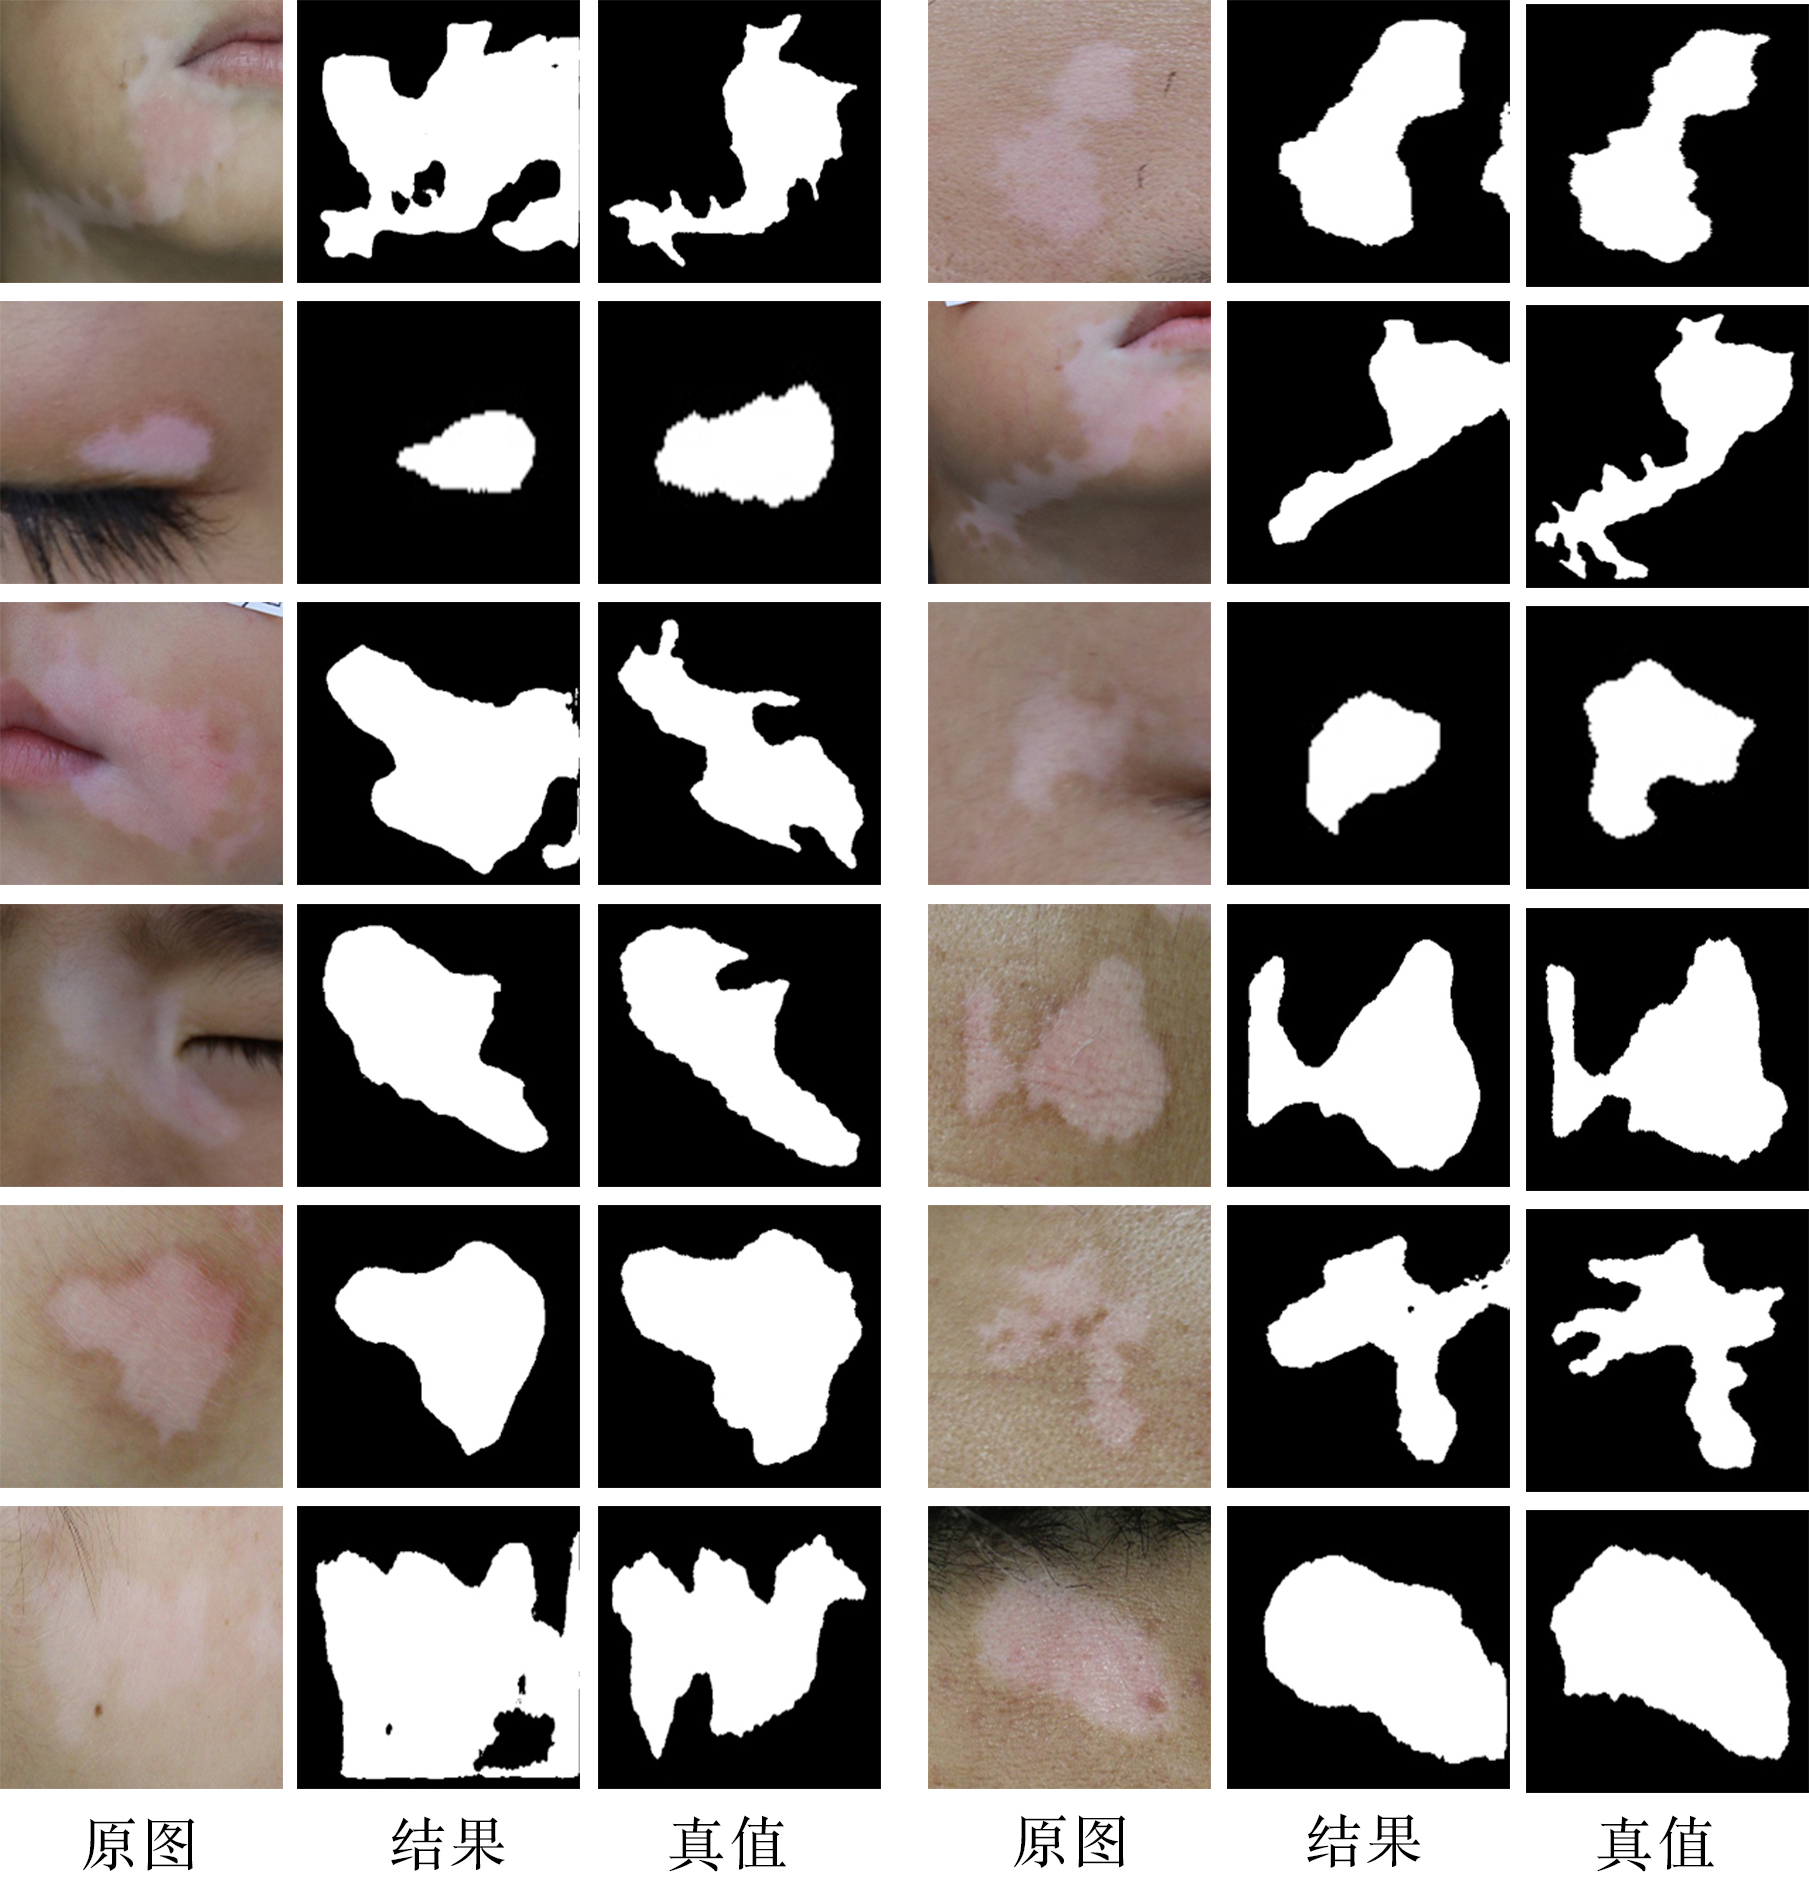
\includegraphics[width=0.7\linewidth]{UnetResult.jpg}
\end{center}
\vspace{-0.5cm}
\caption{Unet部分分割效果图}
\label{fig:UnetResult}
\end{figure}


\section{本章小结}
本章首先介绍了一些近些年来将深度学习应用于图像分割邻域的方法,然后引出了对于强监督学习而言,缺乏大规模的数据集会使得其没有用武之地的观点。于是紧接着介绍了本文所提出的数据集Vit2019,从收集、标注、多样性与挑战四个方面介绍了此数据集,并举例分析了一些样本图片。然后本文并着重介绍了一个经典的网络结构Unet,并且从定量和定性的角度展现并分析了Unet在Vit2019上的效果。在之后的弱监督学习的实验部分,本文也同样对比了强监督方法与现在最先进的弱监督方法的差距,用多项实验说明了本文所提出的弱监督分割方法可以很大程度的缩小与强监督方法之间的鸿沟。
















\chapter{弱监督分割方法及实现}
\section{引言}
机器学习在各种任务中取得了巨大成功,特别是在分类和回归等监督学习任务中。其中分割问题也可以归为分类问题,即对每一个像素进行分类。
%预测模型是从包含大量训练样本的训练数据集中学习,每个训练样本对应一个事件或对象。训练样本由两部分组成:一个描述对象的特征向量,以及一个表示真值输出的标签。
在分类任务中,标签表示训练样本所属的类别;在回归任务中,标签是一个与样本对应的实数值。大多数成功的技术,如深度学习,都需要含有真值标签的大规模训练数据集。然而,在许多任务中,由于数据标注过程的成本极高,很难获得强监督信息。尤其是在医学图像分割领域,获取图像真实值十分的耗时耗力而且容易出错。因此,此领域的研究者十分希望获得能够在弱监督前提下工作的机器学习技术。

目前的弱监督研究领域主要关注三种弱监督类型:不完全监督、不确切监督、以及不准确监督。第一类是不完全监督,即只有训练集的一个(通常很小的)子集是有标签的,其他数据则没有标签。这种情况发生在各类任务中。例如,在图像分类任务中,真值标签由人类标注者给出的。从互联网上获取巨量图片很容易,然而考虑到标记的人工成本,只有一个小子集的图像能够被标注。第二类是不确切监督,即图像只有粗粒度的标签,比如说对图像只有图像类别级的标签。第三种是不准确的监督,模型给出的标签不总是真值。出现这种情况的常见原因有,图片标注者不小心或比较疲倦,或者某些图片就是难以分类。

本文所研究的弱监督属于第二类不确切监督,在接下来的文章当中,本文将不再区别弱监督的类别,而将其默认指代为不确切监督。

\section{方法框架}
本节详细介绍了算法的框架,如图\ref{fig:framework}。在这个框架中,本文采取了一种名为“既见森林,又见树木”的策略。 “森林”是指白癜风本身的特征,“树”是指每个患者的特定皮肤状况(例如,健康的肤色和白癜风的脱色程度)。为了了解白癜风本身的本质,本文训练了一个深度卷积神经网络用于Vit2019的分类。通过查看树,本文利用在推理阶段从输入图像中提取的信息,首先将其分割为超像素,然后在超像素级别上进行提取特征。为了实现“既见森林,又见树木”,本文结合从两方面获得的知识,然后将其作为有用的先验知识引入显着性传播过程。
\begin{figure}[htbp]
\begin{center}
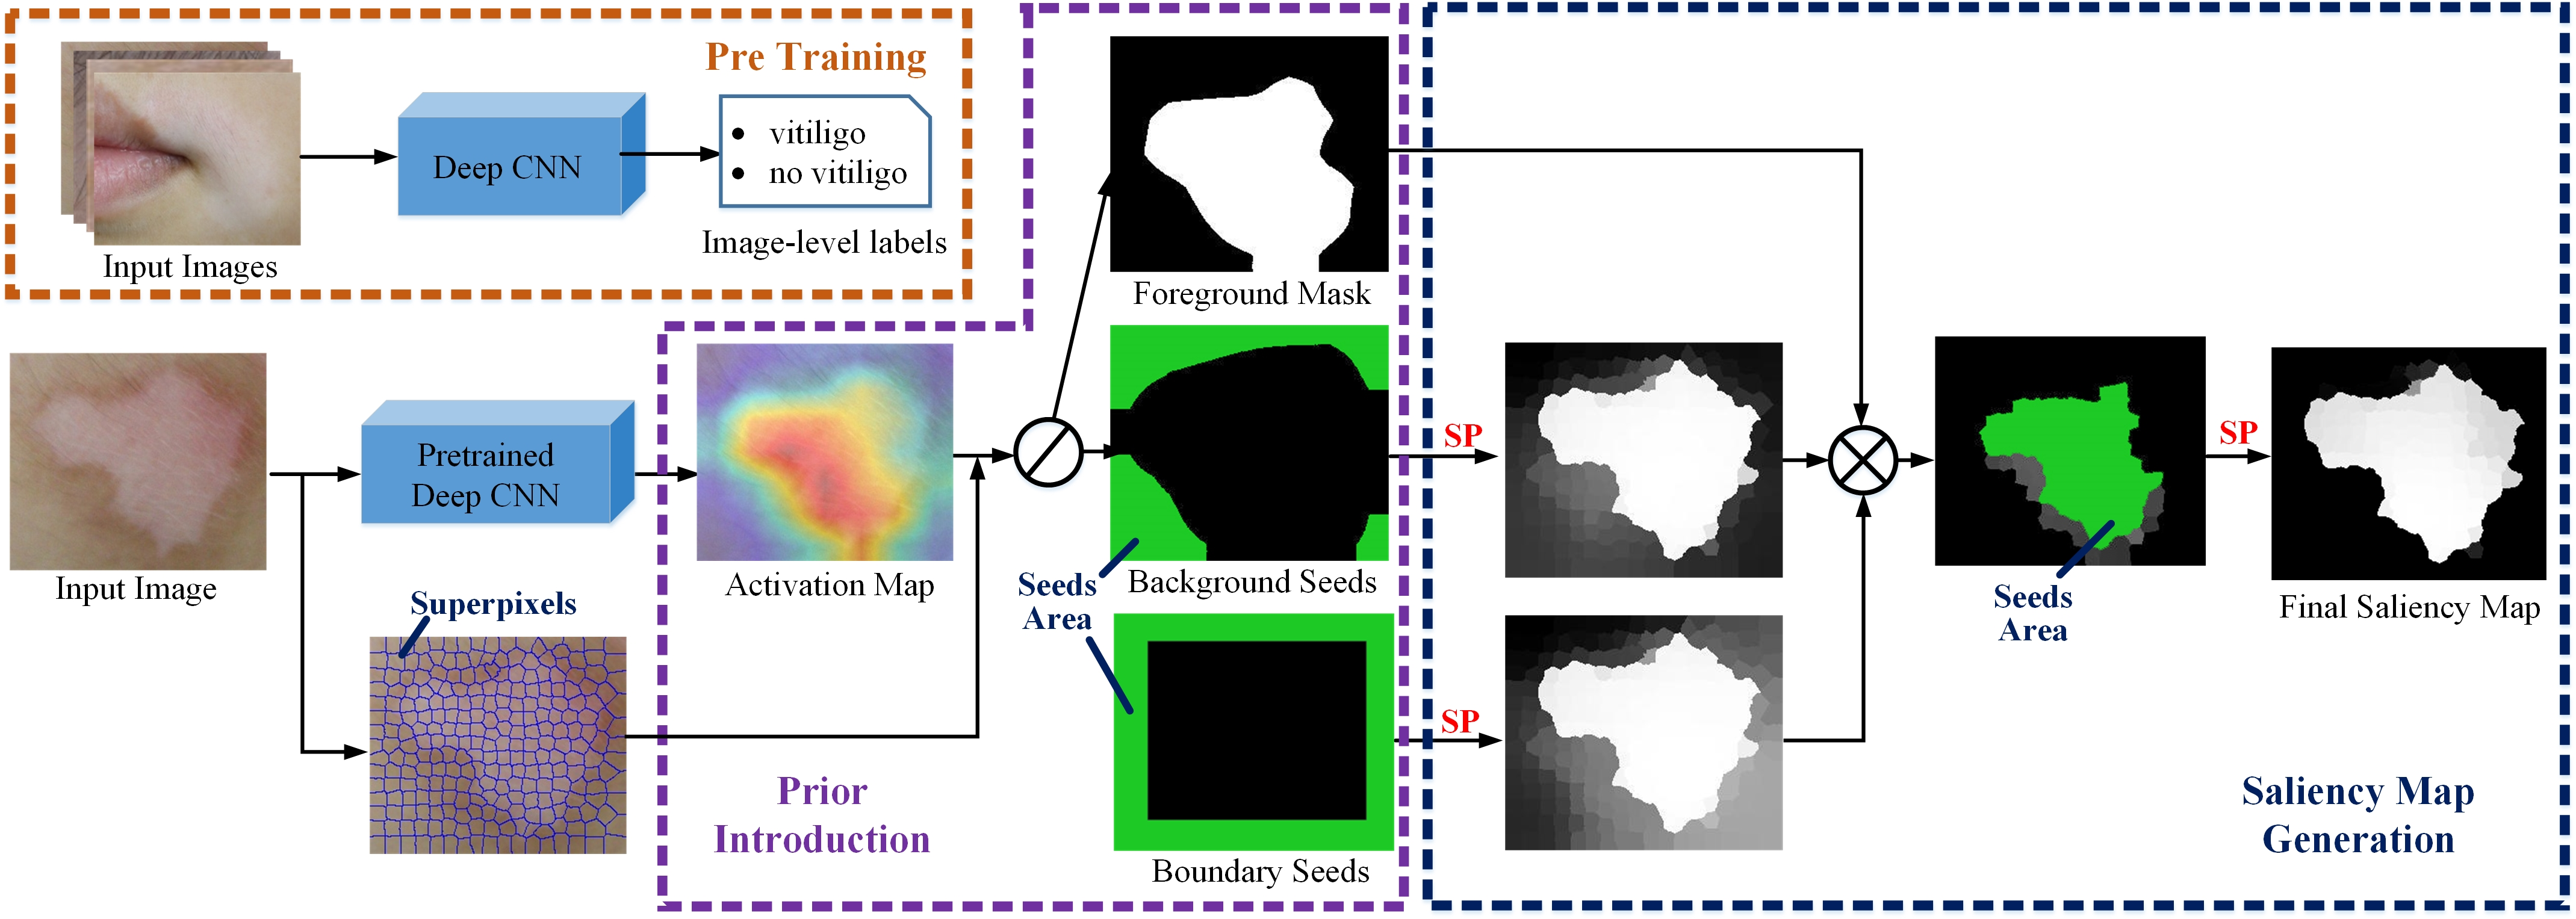
\includegraphics[width=\linewidth]{CNNandSuperPixelModelGraph3.jpg}
\end{center}
   \caption{本文弱监督算法的框架。在第一阶段,训练深度卷积神经网络以识别图像类别。当给定输入图像时,将其分割成超像素;另一方面,使其通过训练好的分类网络以获得激活图。在先验的引入阶段,激活图通过给出种子区域来提供用于显着性传播的先验知识。在显着图生成阶段,本文首先生成一个粗显着图,然后对其进行细化以获得最终显着图. $ \oslash $表示阈值操作。SP 表示在\ref{sec:propagation}节中详述的显着性传播过程。}
\label{fig:framework}
\end{figure}

在接下来的小节中,将详细说明如何通过预先训练的模型获取激活图,如何在超像素上构建图模型,如何通过传播过程生成最后的显著图。

\subsection{预训练分类模型}

本文训练CNN模型来对Vit2019数据集中的图像进行分类,通过简单地在全连接层之前对卷积特征图执行全局平均池化(GAP),利用CNN的副产品---激活图---粗略定位白癜风区域。分类器的准确性可以在一定程度上反映显着图的质量\cite{simonyan2013deep, zhou2016learning}。在这项工作中,本文训练了一个分类错误率为4.27\%ResNet \cite{He_2016_CVPR}的模型。在实践中,当收集新一批图像时,可以使用迁移学习或者微调先前的模型而不是从头开始重新训练。

\subsection{生成类激活图}
只在输出层前(用于分类的softmax)使用全局平均池化层,并将它们作为得出分类的全连接层的特征。通过这种简单的连接结构,可以把图片中的重要区域用输出层权重映射回卷积层特征的方式标记出来,称这种技术为类激活映射(CAM)。如图\ref{fig:CAM}所示,全局平均池化层输出最后一个卷积层的每个单元的特征图的平均值。这些值的加权总和用于生成最后的输出。也可以说,计算最后一个卷积层特征图的加权总和来获得CAM。下面使用更形式化的方式来描述。
\begin{figure}[htbp]
\begin{center}
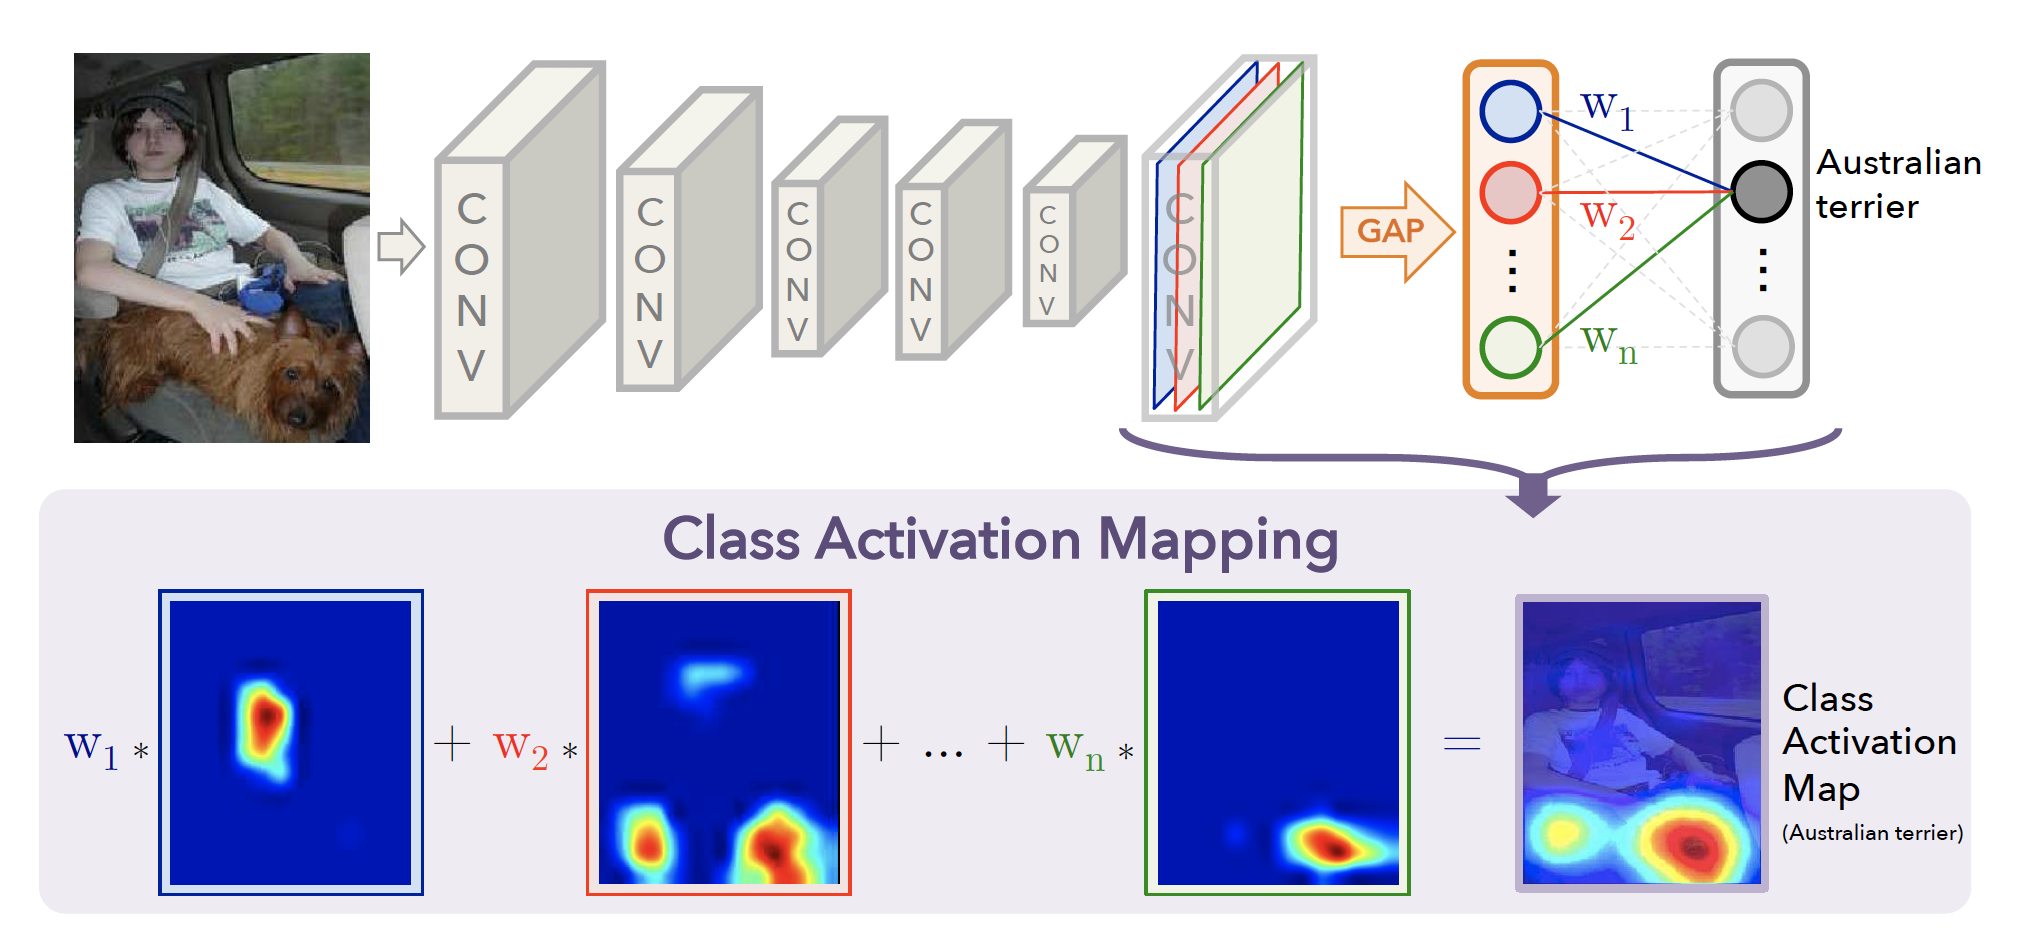
\includegraphics[width=0.9\linewidth]{CAM.png}
\end{center}
\caption{类激活图生成\cite{zhou2016learning}。将预测的类别得分映射回先前的卷积层以生成类显著图(CAMs)。CAM突出了类特定的判别区域。}
\label{fig:CAM}
\end{figure}

对于一个给定的图,用$f_k(x, y)$代表最后一个卷积层在空间坐标$(x,y)$中单元$k$的激活值。然后,对于每个单元$k$,通过GAP后的结果为:
\begin{equation}
\label{eq:chap4_1}
F_k=\sum_{x, y} f_{k}(x, y)
\end{equation}
对于每个类$c$,输入softmax的$S_c$为:
\begin{equation}
\label{eq:}
\sum_{k} w_{k}^{c} F_{k}
\end{equation}
$w_k^c$代表单元$k$对应的类$c$的权重。实际上,$w_k^c$就是$F_k$对类$c$的重要性。最后类$c$的sotfmax输出:
\begin{equation}
\label{eq:}
P_c=\frac{\exp \left(S_{c}\right)}{\sum_{c} \exp \left(S_{c}\right)}
\end{equation}
这里忽略偏差项:明确地把softmax的偏差项设置为0。因为它几乎对分类表现没有影响。
把公式\ref{eq:chap4_1}带入$S_c$,得
\begin{equation}
\label{eq:}
S_{c}=\sum_{k} w_{k}^{c} \sum_{x, y} f_{k}(x, y)=\sum_{x, y} \sum_{k} w_{k}^{c} f_{k}(x, y)
\end{equation}
这里用$M_c$定义类别$c$的CAM,则空间中每个元素为
\begin{equation}
\label{eq:}
M_{c}(x, y)=\sum_{k} w_{k}^{c} f_{k}(x, y)
\end{equation}
因此就有
\begin{equation}
\label{eq:}
S_{c}=\sum_{x, y} M_{c}(x, y)
\end{equation}
所以$M_c(x,y)$直接表明了像素$(x,y)$对网络将图片归类为$c$的贡献。

根据先前的研究\cite{zeiler2014visualizing},研究者都希望用一些可视化方法看到每个被激活的单元的激活区域,$f_k$就是这种可视化方法。简单说CAM就是不同空间区域的线性加权可视化。将类激活图的大小改变成输入图片的大小,就能清楚地看出与特定类最相关的区域。

图\ref{fig:cam}展示了一些作用于白癜风图像上的输出,可以看到属于白癜风区域已经高亮,这说明是这些区域帮助网络将此图片分类为白癜风图片。换一种说法,网络在接收到这张图片后,注意力集中在热度图的红色区域。
\begin{figure}[htbp]
\begin{center}
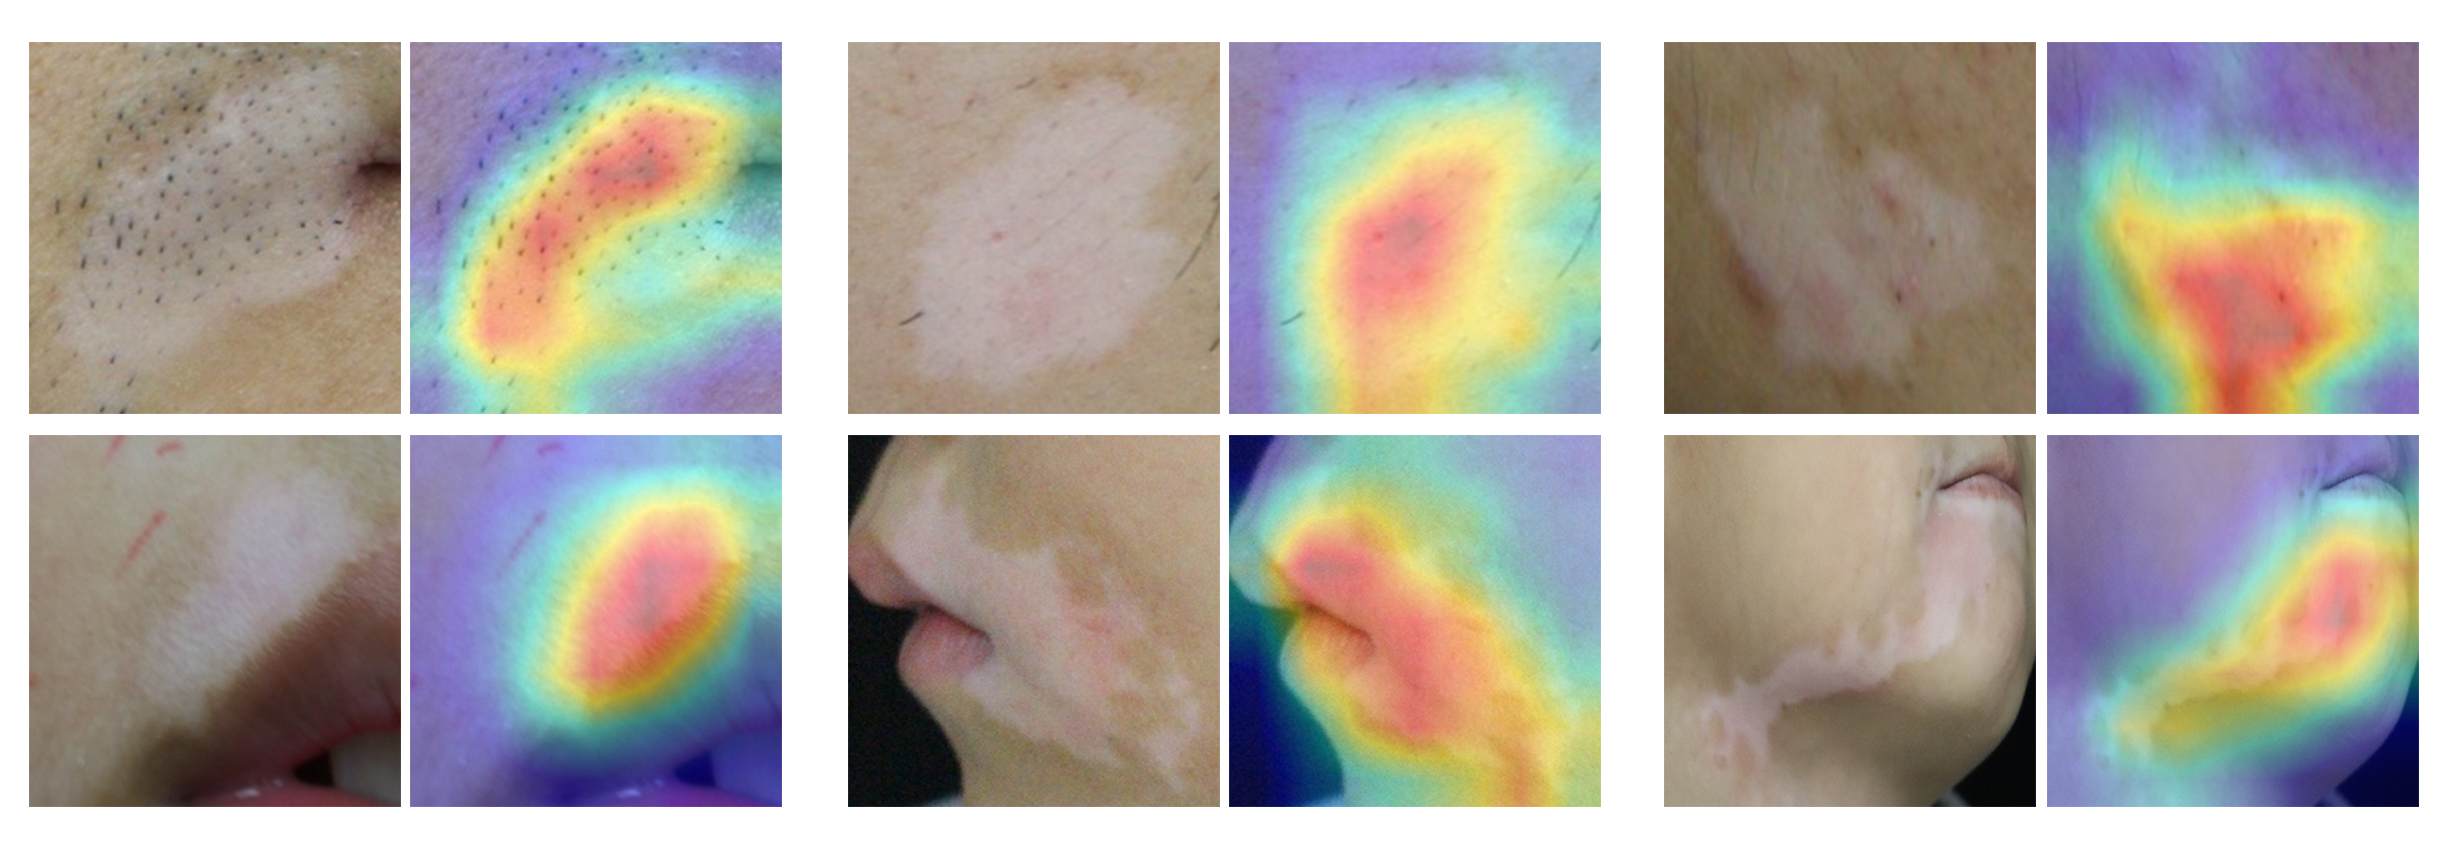
\includegraphics[width=\linewidth]{cam.jpg}
\end{center}
\caption{显著图的示例。蓝色区域表示低的激活值;而红色区域表示高激活值,可以将其视为网络观察到的将整个图像判别为白癜风样本的部分。}
\label{fig:cam}
\end{figure}

全局平均池化(GAP)可能会导致所有响应都很高,因此激活区域通常会过高估计对象的大小\cite{Kolesnikov:2016tf,Zhou:2018ul}。之后本文通过设置一对阈值和灵敏度,巧妙地解决了这个问题,后续的实验论证部分将显示本文的方法不易受激活区域的大小影响。

\subsection{图构建}
通过使用第\ref{sec:SLIC}章中所介绍的SLIC算法,本文将输入图片分割成$N$个小的超像素,然后建立无向图$\mathcal{G}=\langle \mathcal{V},\mathcal{E}\rangle$, 其中$\mathcal{V}$是顶点集合,包含这些超像素,$\mathcal{E}$是边集,对他们之间的相似性进行编码. 在本文的工作中,如果两个节点$\mathbf{s}_i$和$\mathbf{s}_j$在空间中相邻或者对应于边缘超像素我们就在其间建立一条边。他们的相似性由高斯核函数进行度量
\begin{equation}
\label{eq:}
\omega_{ij}=\exp{\Big (\frac{ -\| \mathbf{s}_i-\mathbf{s}_j \| ^2} { (2\theta^2)} \Big )}
\end{equation}
, 其中$\theta$是核宽度。并且 $\mathbf{s}_i$ 是第 $i$个超像素在LAB-XY空间中的特征向量,即$(\mathbf{s}_i^{color};\mathbf{s}_i^{position})$。因此可以得到图 $\mathcal{G}$的临接矩阵$\mathbf{W}\in\mathbb{R}^{N\times N} $ 这里定义其为$\mathbf{W}_{ij}=\omega_{ij}$ 如果 $i\neq j$, 否则 $\mathbf{W}_{ij}=0$。 对角矩阵是$\mathbf{D}$,定义为 $\mathbf{D}_{ii} =\Sigma_j \mathbf{W}_{ij}$。

至此,本文建立了在超像素基础上的图结构。

\subsection{先验引入}
在本节中,将详细介绍如何利用显著图提供的先验知识,并通过显着性传播过程构建最终显着图。

首先为类显著图$M_{(c=1)}$定义两个阈值$ {T_\mathrm f}$ 和 $ {T_\mathrm b}$ 来获得前景区域$\mathcal{R}_\mathrm{f} $  和背景区域 $\mathcal{R}_\mathrm{b}$ :
\begin{IEEEeqnarray}{rCl}
\label{eq:2}
\mathcal{R}_\mathrm{f} & = &\{ (x,y) \mid M_{(c=1)}(x,y)\geq \mathrm{PERC}_{T_\mathrm{f}}(M_{(c=1)}) \}\,,  \nonumber \\ 
\mathcal{R}_\mathrm{b} & =& \{ (x,y) \mid M_{(c=1)}(x,y)\leq \mathrm{PERC}_{T_\mathrm{b}}(M_{(c=1)}) \}\,, \\
&\mathrm{s.t. }& \quad {T_\mathrm f}-{T_\mathrm b}\geq 0 \,.\nonumber
\end{IEEEeqnarray}
在公式~\eqref{eq:2}中, 函数$\mathrm{PERC}_{T_\mathrm{f}}(\cdot)$ 表示首先将$(\cdot)$ 中的元素从小到大进行排序,然后函数返回第 ${T_\mathrm f}$百分位的值。直观上讲,$\mathcal{R}_\mathrm{f}$ 主要关注点在于前景区域,即本文中的白癜风区域,然而 $\mathcal{R}_\mathrm{b}$ 主要关注点在非前景区域,即非白癜风、拍摄环境背景。本文限制 ${T_\mathrm f}-{T_\mathrm b}\geq 0$ 主要目的是使得 $\mathcal{R}_\mathrm{f}$  $\mathcal{R}_\mathrm{b}$ 更加的纯净, 这样做会方便进行接下来的显著性传播。

\subsection{显著图构建}
我们为在前景区域 中的 $\mathbf{s}_i$生成前景掩模 $F_\mathrm{Mask}$,其中如果$(s_i^x,s_i^y) \in \mathcal{R}_\mathrm{f}$则 $F_\mathrm{Mask}{(i)}=1$, 否则 $F_\mathrm{Mask}{(i)}=0$。 我们将$\mathcal{R}_\mathrm{b}$ 当做背景种子区域,并且当做第一次显著性传播开始的区域,显著性值通过传播过程将传播至其余区域。我们将显著性传播过程的结果看做一个 $N$维的向量  $\mathbf{sp}^*=(sp_1^* \cdots sp_N^*)$ ,其中 $N$是超像素的个数, $ sp_i^*\,(i=1, \cdots,N)$ 是对应于超像素 $\mathbf{s}_i$的显著性值. 在将 $\mathbf{sp}^*$ 归一化到 $[0,1]$之后, 第$i$个在$S_\mathrm{Bg}$ 中 的超像素的值是:
\begin{equation}
\label{eq:3}
S_\mathrm{Bg}(i)=1-\mathbf{sp}^*_\mathrm{normalized}(i),i=1,2,\cdots,N.
\end{equation}
此外,边界先验被引入到显着性传播过程,其假设:

沿着图像的四个边界的区域通常是非目标对象。

这种假设可以在大多数临床情况下得到满足,因为医生总是倾向于将病变区域放在最明显的区域(即中心)。因此,类似于 $S_\mathrm{Bg}$,我们将显着性值从边界种子区域中的超像素传播到其他超像素,以获得显着性图$S_\mathrm{Bnd}$。

最终我们结合得到的$S_\mathrm{Bg}$, $S_\mathrm{Bnd}$ 和 $F_\mathrm{Mask}$ 生成粗略的显著图$S_\mathrm{Coarse}$:

\begin{equation}
\label{eq:4}
S_\mathrm{Coarse}(i)=S_\mathrm{Bg}(i) \otimes S_\mathrm{Bnd}(i) \otimes F_\mathrm{Mask}(i),
\end{equation}
其中 ``$\otimes$'' 表示两个向量之间的元素的乘积运算 。

其中 $F_\mathrm{Mask}$主要包含背景区域, 我们从潜在的前景区域中选择具有较大显著性值的超像素,从而将背景区域尽可能的排除在外:
\begin{equation}
\label{eq:5}
\{ \mathbf{s}_i \mid S_\mathrm{Coarse}(i) \geq \eta \max_{1\leq j\leq N}{(S_\mathrm{Coarse}(j))}\},
\end{equation}
其中 $\eta$ 是一个自定义的选择率。然后我们将这些超像素作为下一次显著性传播过程的种子点,并进一步的抑制背景区域并加强前景区域。最终我们便可以得到显著性图$S_\mathrm{Final}$.

\section{显著性传播过程}\label{sec:propagation}
\begin{figure}[htbp]
\begin{center}
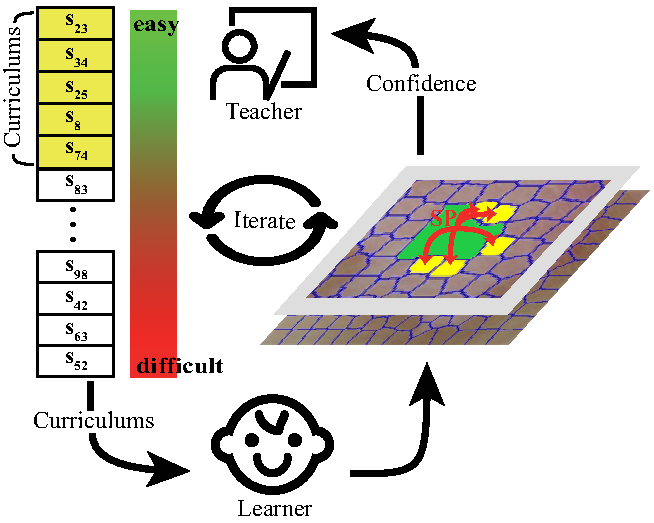
\includegraphics[width=0.7\linewidth]{TLLTillustrator.pdf}
\end{center}
\caption{显着性传播过程。在左侧,教师选择几个最简单的节点(黄色)作为学习者的课程。然后,学习者通过显着性传播“学习”这些节点。在右侧,学习者向教师提供反馈(即信心),以帮助教师确定下一个课程的数量。}
\label{fig:TLLTillustrator}
\end{figure}

显著性传播方法在我们的算法中非常重要. 假设我们在图$\mathcal{G}$中有$l$个种子节点$\mathbf{s}_1,\cdots , \mathbf{s}_l$, 其值为$f_1=\cdots = f_l =1$, 显著性传播的任务是将显著性值准确可靠从这些已经标记的$l$个节点传播到剩余的$u=N-l$个未被标记的超像素。
然而现有方法的传播顺序可能在处理较复杂的超像素时产生瑕疵,所以本文基于自动控制原理中的反馈思想,在原先框架上优化学习顺序(见图\ref{fig:TLLTillustrator})。

具体来说,这个框架由学习者和教师组成。 给定在时间$t$标记的集合$\mathcal{L}^{(t)}$和未标记的集合$\mathcal{U}^{(t)}$,老师从中$\mathcal{U}^{(t)}$选择一组简单的超像素作为为课程$\mathcal{T}^{(t)}$。 然后,学习者将学习$\mathcal{T}^{(t)}$,并将反馈返回给老师以帮助老师更新$(t + 1)$次学习的课程。 这个过程迭代直到$\mathcal{U}^{(t)}$中的所有超像素都被传播到。

\subsection{``教学''过程}
``教学''过程的核心在于设计一个老师,这个老师可以决定哪些未被标记的超像素在接下来的过程中被学生学习。对于第$t$次传播过程,首先建立一个候选集$\mathcal{C}^{(t)}$,其中元素是在图$\mathcal{G}$中直接与$\mathcal{L}^{(t)}$相邻的超像素。然后教师从$\mathcal{C}^{(t)}$中选择最简单的几个元素作为第$t$次的课程。为了衡量超像素$\mathbf{s}_i \in \mathcal{C}^{(t)}$ 的传播难度,我们定义难度系数$DS_i$
\begin{equation}
DS_i=INF_i+IND_i+IHM_i+CON_i
\end{equation}
其中$INF_i$度量信息性,$IND_i$度量个体性,$IHM_i$度量不同质性,$CON_i$度量连通性。接下来本文详细的介绍每一种度量的定义。

\textbf{信息性:}在给定集合$\mathcal{L}$之后,简单的超像素不应该再引入过多的信息,于是一个超像素$\mathbf{s}_i \in \mathcal{C}$的信息性度量可以直接使用条件熵$H(\mathbf{s}_i \mid \mathcal{L})$进行建模,表示为:
\begin{equation}
INF_i=H(\mathbf{s}_i \mid \mathcal{L})
\end{equation}
这个传播过程遵循多元高斯过程,在随机向量$\mathbf{f}=(f_1 \cdots f_N)^ \mathrm{T}$中的元素$f_i(i=1, \cdots ,N)$代表超像素$\mathbf{s}_i$的显著值。相关协方差矩阵$\mathbf{K}$相当于将邻接矩阵$\mathbf{W}$的对角线元素全部置为$1$.
对于多元高斯,$H(\mathbf{s}_i \mid \mathcal{L})$闭式表达为:
\begin{equation}
INF_i=H(\mathbf{s}_i \mid \mathcal{L})=\frac{1}{2}\ln{(2 \pi e \sigma_{i \mid \mathcal{L}}^2)}
\end{equation}
其中$\sigma_{i \mid \mathcal{L}}^2$是给定$\mathcal{L}$后$f_i$的条件协方差,考虑到条件分布是一个多元高斯,$\sigma_{i \mid \mathcal{L}}^2$可以表达成
\begin{equation}
\label{eq:7}
\sigma_{i \mid \mathcal{L}}^2=\mathbf{K}_{ii}^2-\mathbf{K}_{i,\mathcal{L}} \mathbf{K}_{\mathcal{L},\mathcal{L}}^{-1} \mathbf{K}_{\mathcal{L},i},
\end{equation}
其中$\mathbf{K}_{i,\mathcal{L}} $和$\mathbf{K}_{\mathcal{L},\mathcal{L}} $表示$\mathbf{K}$的子矩阵。通过带入消元,我们得到$\mathbf{s}_i$
在\eqref{eq:7}中对$\mathbf{K}_{\mathcal{L},\mathcal{L}}$求逆的步骤在每一次迭代过程都需要进行计算,随着集合$\mathcal{L}$越来越大,直接求逆非常的耗费时间,因此一种高效的基于块的更新方法在补充材料中进行了推导。

\textbf{个体性:} 个体性衡量一个超像素与其周围邻居超像素有多么不同.我们认为一个简单的超像素与周围的超像素具有相似的LAB 颜色空间。一个超像素个体性度量越小,则说明与其周边超像素越相近。
\begin{equation}
\label{eq:8}
IND_i=IND(\mathbf{s}_i,{\mathcal{N}(\mathbf{s}_i)})=\frac{1}{|\mathcal{N}(\mathbf{s}_i)|}\sum_{j\in \mathcal{N}(\mathbf{s}_i)}\| \mathbf{s}_i^{\mathrm color}-\mathbf{s}_j^{\mathrm color}\|,
\end{equation}
其中$\mathcal{N}(\mathbf{s}_i)$表示$\mathbf{s}_i$邻居的数目

\textbf{同质性:}显然,对于一个不同质的超像素来说,其中包含的像素是多样的、不统一的。假设在超像素$\mathbf{s}_i$中有$b$个像素$\{\mathbf{p}_j^{\mathrm color}\}^b_{j=1}$,向量的维度代表LAB颜色特征。然后将他们的相关性记录在一个$b \times b$的对称矩阵$\pmb{\Theta}=\mathbf{P}\mathbf{P^{\mathrm T}}$,其中矩阵$\mathbf{P}$的每一行代表了一个像素的特征向量$\mathbf{p}_j^{\mathrm color}$的转置,因此超像素$\mathbf{s}_i$的$IHM_i$定义为:
\begin{equation}
\label{eq:9}
IHM_i=\Big (\frac{2}{b^2-b}\sum_{i=1}^b \sum_{j=i+1}^b\pmb{\Theta}_{ij}\Big )^{-1}
\end{equation}
其中$\pmb{\Theta}_{ij}$是矩阵$\pmb{\Theta}$的第$(i,j)$个元素,一个较小的$IHM_i$意味着超像素$\mathbf{s}_i$中的所有像素都很相似,并且可以很容易被学习者学习。

\textbf{连通性:}对于已经建立的图$\mathcal{G}$来说,一个直觉是与集合$\mathcal{L}$连接性强的超像素并不难进行传播。于是超像素$\mathbf{s}_i \in \mathcal{C}$与集合$\mathcal{L}$中的所有元素的测地距离与其连通性度量成反比例关系。
\begin{equation}
\label{eq:10}
CON_i=\frac{1}{l}\sum_{j\in \mathcal{L}}\mathrm{geo}({\mathbf{s}_i,\mathbf{s}_j})
\end{equation}
在\eqref{eq:10}中,$\mathrm{geo}({\mathbf{s}_i,\mathbf{s}_j})$表示$\mathbf{s}_i$与$\mathbf{s}_j$之间的测地距离,可以使用最短路径进行近似:
\begin{IEEEeqnarray}{rCl}
\label{eq:11}
\mathrm{geo}({\mathbf{s}_i,\mathbf{s}_j})&=\min_{R_1=i,R_2,\cdots,R_n=j}\sum_{k=1}^{n-1}\max{({E_{R_k,R_{k+1}}-c_0},0)}  \\
\mathrm{s.t.} & R_k,R_{k+1} \in \mathcal{V}, R_k\mbox{和}R_{k+1}\mbox{相邻} \nonumber
\end{IEEEeqnarray}
此处$\mathcal{V}$代表$\mathcal{G}$的顶点集,$E_{R_k,R_{k+1}}$计算了$R_k$和$R_{k+1}$的欧式距离,其中$c_0$是一个自适应阈值,用来防止``小权重积累问题''.

最终,通过公式代换,我们得到了所有$\mathbf{s}_i \in \mathcal{C}$的难度系数,在老师的帮助下,未被标记的超像素逐渐从简单到复杂的学习。

\subsection{反馈过程}
在计算了所有候选超像素的难度系数之后,下一步便是选取特定数量的超像素作为课程。一个直接的想法是,将元素从小到大排序后选择前$q \,(q\leq |\mathcal{C}|)$个用来建立课程集合$\mathcal{T}=\{\mathbf{s}_1,\mathbf{s}_2,\cdots,\mathbf{s}_q\}$但我们认为在第$t$次所学的数目应该由第$t-1$次所学效果决定:如果第$t-1$次学习过程比较自信,那么教师会分派更多的学习任务给学习者。也就是说,教师应该考虑学习者的反馈来调节课程量。于是我们使用自适应的$q^{(t)}$作为第$t$次所学的课程量。

正如上面所讲,$q^{(t)}$应该被前一次的学习过程所决定。但是因为第$t-1$次学习的正确性无从得知,于是本文定义了置信值来估计此前的学习效果。直观上讲,如果显著值$f_1^{t-1},\cdots, f_{q^{(t-1)}}^{(t-1)}$在归一化之后接近$0$\,(与种子点非常不相似)\,或者$1$\,(与种子点极为相似),则认为第$t-1$次学习的置信度高,相反如果$f_1^{t-1},\cdots, f_{q^{(t-1)}}^{(t-1)}$接近$0.5$,这意味着此学习的置信度低,于是第$t$次应该使用一个更小的$q^{(t)}$。于是置信度(属于$[0,1]$之间)定义为:
\begin{equation}
\label{eq:12}
\mathrm{ConfidenceScore}=1-\frac{2}{q^{(t-1)}}\sum_{i=1}^{q^{(t-1)}}\min{(f_i^{(t-1)},1-f_i^{(t-1)})}, 
\end{equation}
最终可以计算出来$q^{(t)}$:
\begin{equation}
\label{eq:13}
q^{(t)}={|\mathcal{C}^{(t)}|\times \mathrm{ConfidenceScore}}.
\end{equation}

\subsection{显著性传播过程}
当课程$\mathcal{T}=\{\mathbf{s}_1,\mathbf{s}_2,\cdots,\mathbf{s}_{q^{(t)}}\}$确定了之后,学习者通过传播过程将显著值从$\mathcal{T}^{(t)}$传播到$\mathcal{L}^{(t)}$,可表达为:
\begin{equation}
\label{eq:14}
\mathbf{f}^{(t+1)}=\mathbf{M}^{(t)}\mathbf{D}^{-1}\mathbf{W}\mathbf{f}^{(t)}
\end{equation}

其中$\mathbf{M}$是一个对角线矩阵,如果$\mathbf{s}_i\in \mathcal{T}^{(t)}\cup \mathcal{L}^{(t)}$,
那么令$\mathbf{M}_{ii}^{(t)}=1$,否则$\mathbf{M}_{ii}^{(t)}=0$,当第$t$步迭代完成了之后,被标记和未被标记的集合更新为$\mathcal{L}^{(t+1)}=\mathcal{L}^{(t)} \cup \mathcal{T}^{(t)}$,$\mathcal{U}^{(t+1)}=\mathcal{U}^{(t)} \setminus \mathcal{T}^{(t)}$.

以$\mathbf{f}^{(0)}=\Big (f_1^{(0)},\cdots,f_N^{(0)}\Big)$初始化公式\ref{eq:14}, 如果第$i$个超像素对应于种子点,则令$f_i^{(0)}=1$,否则令$f_i^{(0)}=0$。当集合$\mathcal{U}$为空时终止,得到显著值向量$\mathbf{f}$。

\section{实验结果与分析}
在本节中,首先在定性上将本文的方法与TLLT \cite {gong2015saliency}进行比较,并说明本文的优势。然后,定性和定量地比较本文的方法与现有技术,并讨论失败的案例。然后进行简化模型研究,即通过化简模型来讨论模型中每一个步骤的必要性,并进行参数灵敏度分析。本文在整个实验中使用以下参数:$ {N_\mathrm {max}} = 400, T_\mathrm {f} = 30, {T_ \mathrm {b}} = 60, \theta = 0.25, \eta = 0.4 $ 。


\subsection{注意力机制验证}
在\cite{gong2015saliency}中,凸包提取与检测用于粗略定位特征对象。然而,它总是具有误导性(见图 \ref {fig:TLLT}),因为与面部的其他部位(例如,鼻子,嘴唇,眉毛,眼睛)相比,白癜风不是一个显着的对象。相比之下,本文从类感知激活图中引入了先验,这可以帮助我们正确地关注于我们关心的对象。

\begin{figure}[htbp]
\begin{center}
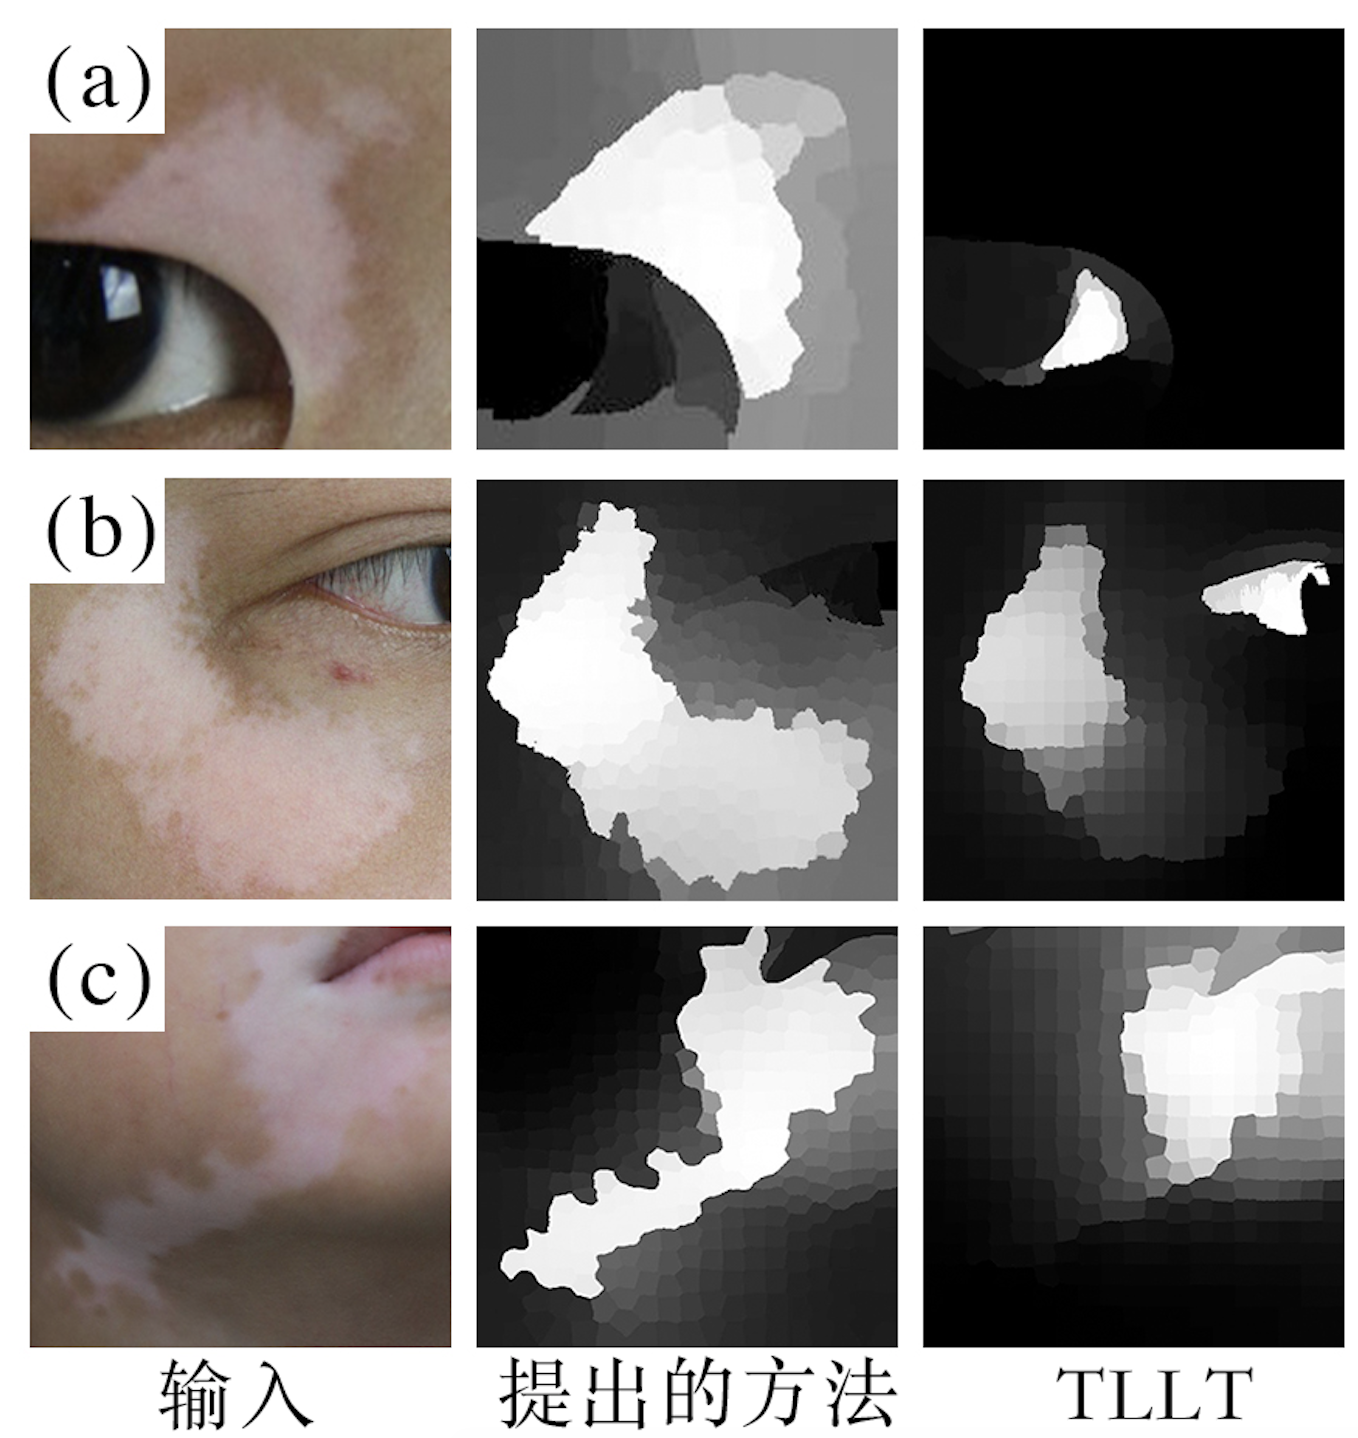
\includegraphics[width=0.6\linewidth]{TLLT.png}
\end{center}
\caption{与TLLT的效果对比。在每行中,从左到右的图像分别代表原始图像、本文的方法的结果和TLLT的结果。 (a)和(b)显示TLLT专注于错误的地方,而本文的方法可以正确地专注于白癜风区域。(c)显示本文的方法可以很好地抑制背景并使前景脱颖而出。}
\label{fig:TLLT}
\end{figure}

为了逐渐将注意力集中在我们感兴趣的物体上,本文通过引入几个先验来抑制背景,从而使前景突出。为了量化这个过程,本文借用了信噪比的概念。也就是说,根据真值图像,显着性值位于白癜风区域被认为是一个有用的信号,而显着性值在非白癜风区域则被视为无用的噪音信号。我们将其表述为:
\begin{equation}
\label{eq:16}
\mathrm{SNR_{dB}}=10\mathrm{log_{10}}(\frac{E_{\mathrm{signal}}}{E_{\mathrm{noise}}}),
\end{equation}

其中 $E_\mathrm{signal}$ 和 $E_\mathrm{noise}$ 分别是信号和噪声的能量项, 由显著性值的均方差所度量。 统计结果参见图\ref{fig:SaliencySNR}. 如果将 $\mathrm{SNR_{dB}}=0$ 作为基准线,可以发现在引入先验之后,显著性图的信噪比$S_\mathrm{Bg}$ 和 $S_\mathrm{Bnd}$均有所增加。然后通过结合细化显著性图的步骤,我们最终得到的显著性图$S_\mathrm{Final}$的信噪比有了非常大的提升($2.08$ dB)。
 
\begin{figure}[htbp]
\begin{center}
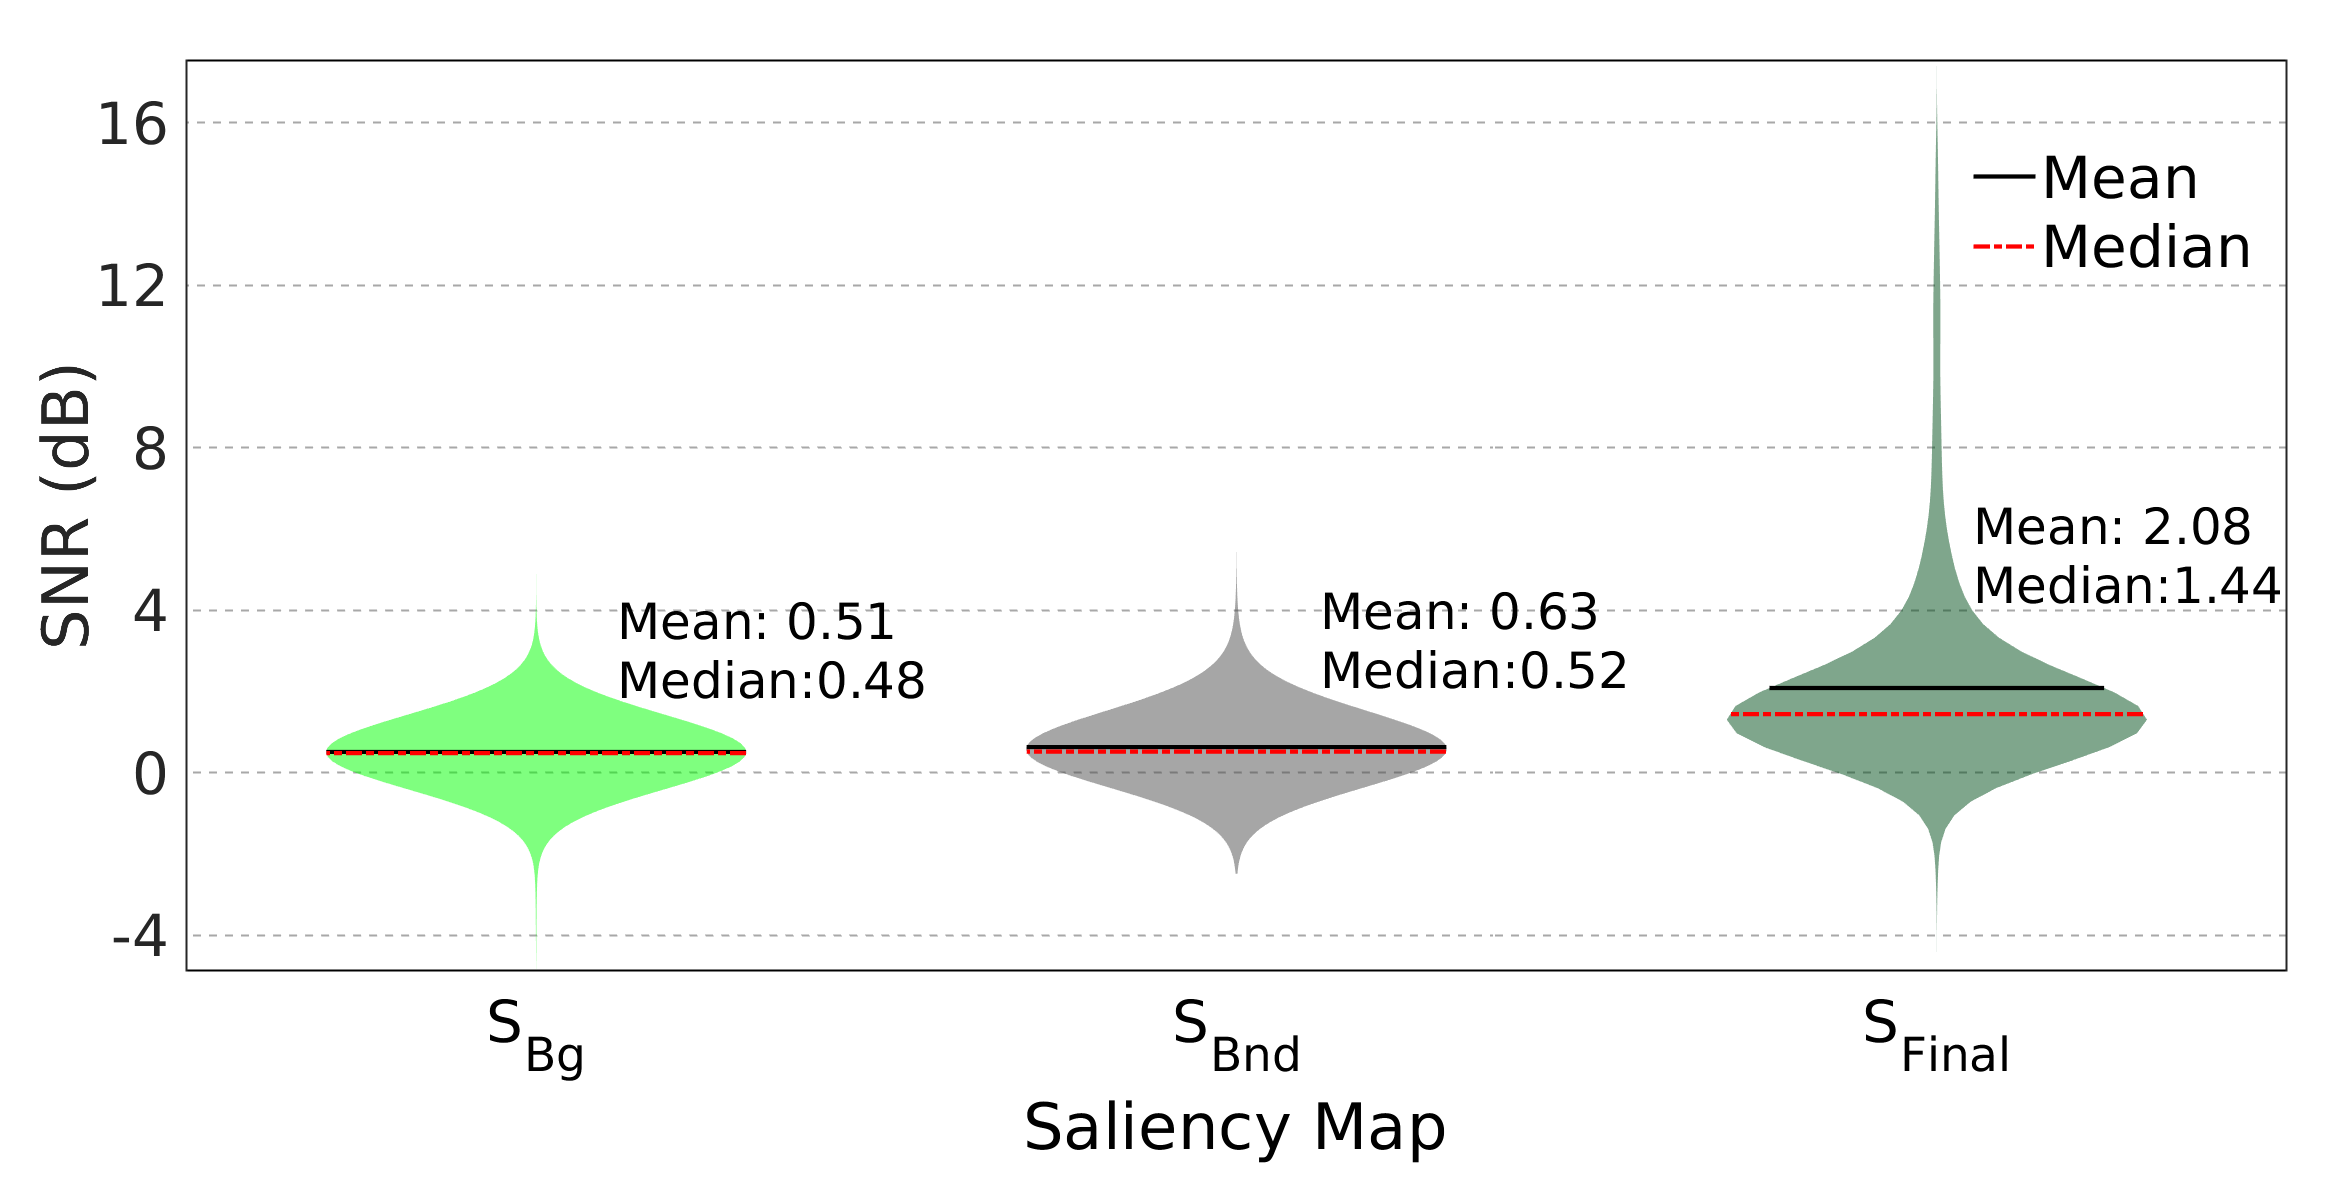
\includegraphics[width=0.8\linewidth]{VitViolin.eps}
\end{center}
\caption{三个显著性图的信噪比,即 $S_\mathrm{Bg}$, $S_\mathrm{Bnd}$ 和 $S_\mathrm{Final}$.}
\label{fig:SaliencySNR}
\end{figure}

\subsection{分割效果的定量与定性分析}
\textbf{定量分析}

给定输入图像,本文的算法产生具有若干灰度级的显著图。为了与不同的分割方法进行比较,设置阈值($ {T_ \mathrm {bin}} = 0.5 $)最终获得二元掩模。本文采用IoU来评估算法的性能。

\begin{table}[tbp]
  \begin{center}
  \caption{全监督学习与弱监督学习在Vit2019数据集上的表现,以IoU (\%)为衡量标准}
    \begin{tabular}{c|c|c}
    \toprule
   方法 & 监督形式 & mIoU \\
    \hline
    \hline
    FCN-VGG16\cite{long2015fully}  & \multirow{2}[2]{*}{Fully} & 72.4 \\
    U-net\cite{ronneberger2015u} &       & 78.6 \\
    \hline
    PRM\cite{Zhou:2018ul}   & \multirow{3}[2]{*}{Weakly} & 67.2 \\
    SEC\cite{Kolesnikov:2016tf}   &       & 64.7 \\
    Our Method &       &\textbf{71.4}\\
    \bottomrule
    \end{tabular}%
\end{center}
  \label{tbl:CompareResult}%
\end{table}%

在表4.1中,本文首先将两种典型的完全监督方法U-net和FCN在Vit2019上进行测试,然后与最先进的弱监督方法进行比较,即 \cite{Zhou:2018ul, Kolesnikov:2016tf}。本文的方法使用图像级标签和标准设置来训练分类模型,而没有使用CRF后处理\cite{Kolesnikov:2016tf}或生成可能的切割面片的方法\cite{Zhou:2018ul},并通过阈值操作直接生成二进制掩码并显现了有竞争力的结果。可以看出,本文的方法在一定程度上优于其他弱监督方法,并减小了弱监督和全监督方法效果之间的差距。

\textbf{定性分析}

首先,与表4.1中的完全监督方法相比,虽然本文的表现一般较差,但在一些具有挑战性的图片中,本文的方法优于U-net,如图~\ref {fig:unetResult}。在低对比度条件下,本文的方法可以更好地定位皮肤病变区域,显著图本身可以更好地反映健康皮肤和白癜风皮肤之间的过渡区域。对于包含毛发脱色的部分,也可以在得到的二元掩模图像中得到反映。对于某些高光区域,例如嘴唇上的反射,我们的方法也可以降低误报率。而且,我们的方法可以更好地保留边缘的细节。

\begin{figure}[htbp]
\begin{center}
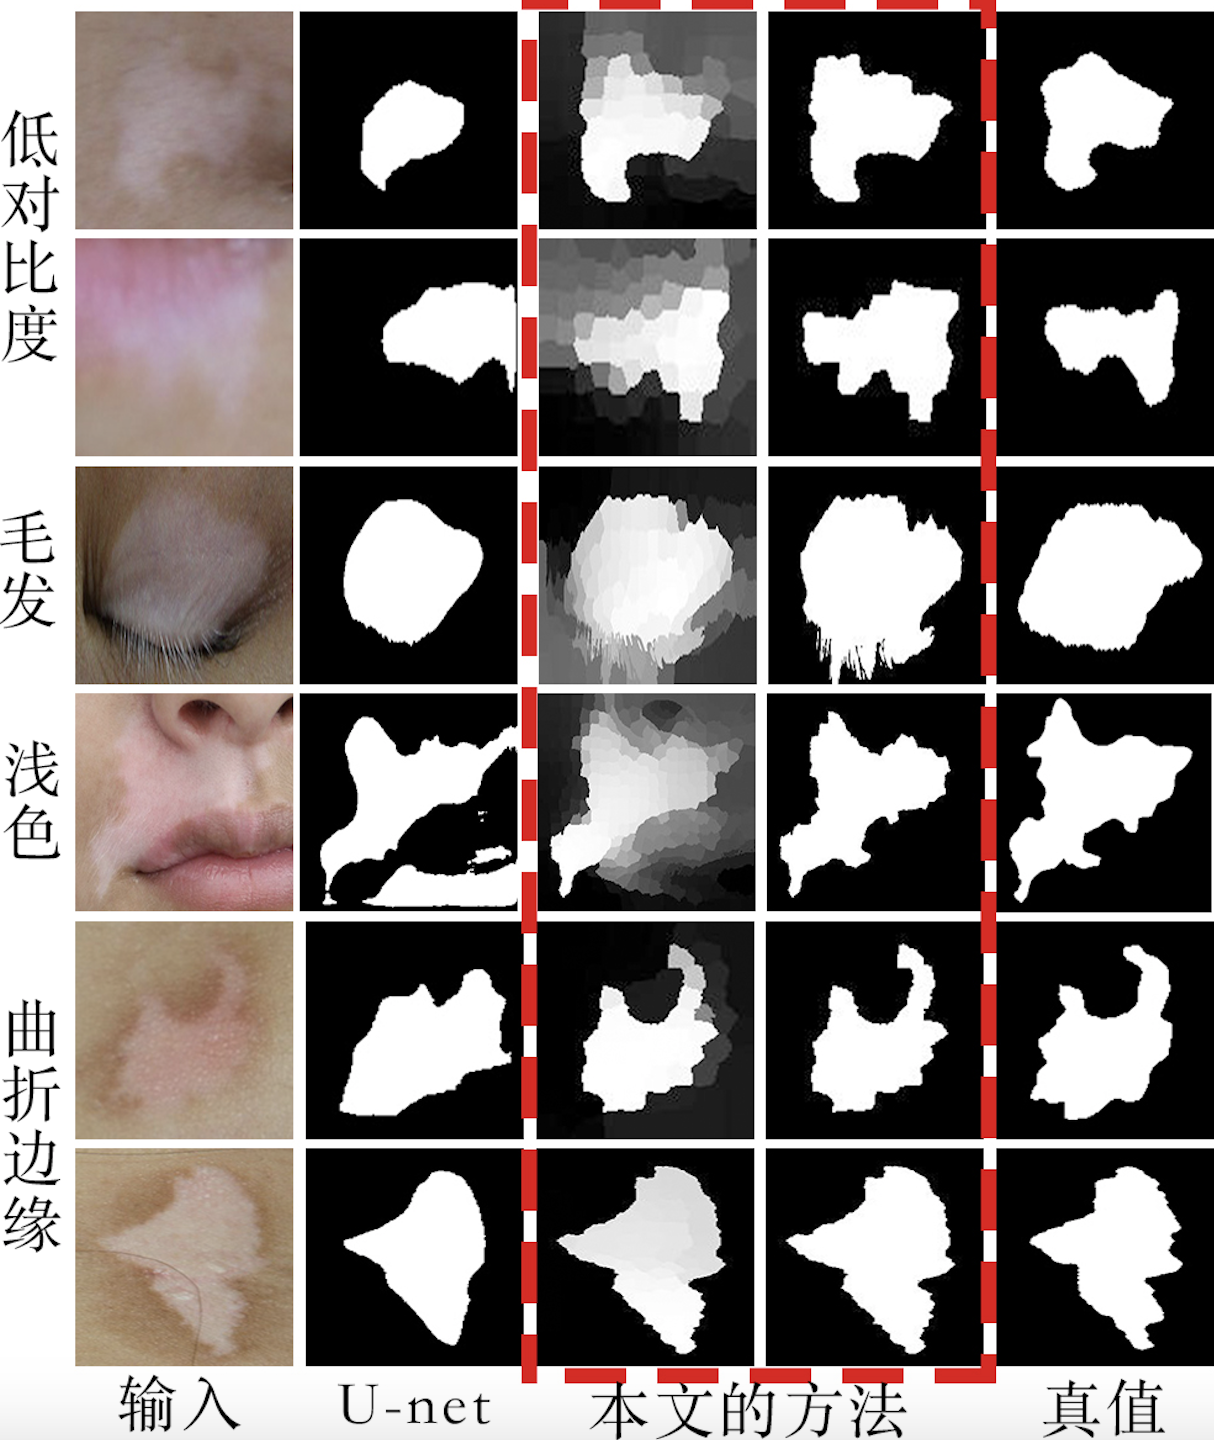
\includegraphics[width=0.7\linewidth]{unetcompareSmaller.png}
\end{center}
   \caption{U-net和我们的方法生成的掩码的可视化比较。在使用$ {T_ \mathrm {bin}} $对本文方法所获得的显着性图(红色虚线框中的第一列)进行阈值处理后,我们可以获得二元掩模(框中的第二列)。真值(GT)在最后一栏中给出。}
\label{fig:unetResult}
\end{figure}

其次,与最先进的弱监督方法相比,如图\ref {fig:weaklySupervisedCompare}所示,我们的方法可以保持较好的边界,并在恶劣条件下保持鲁棒性。

\begin{figure}[h]
\begin{center}
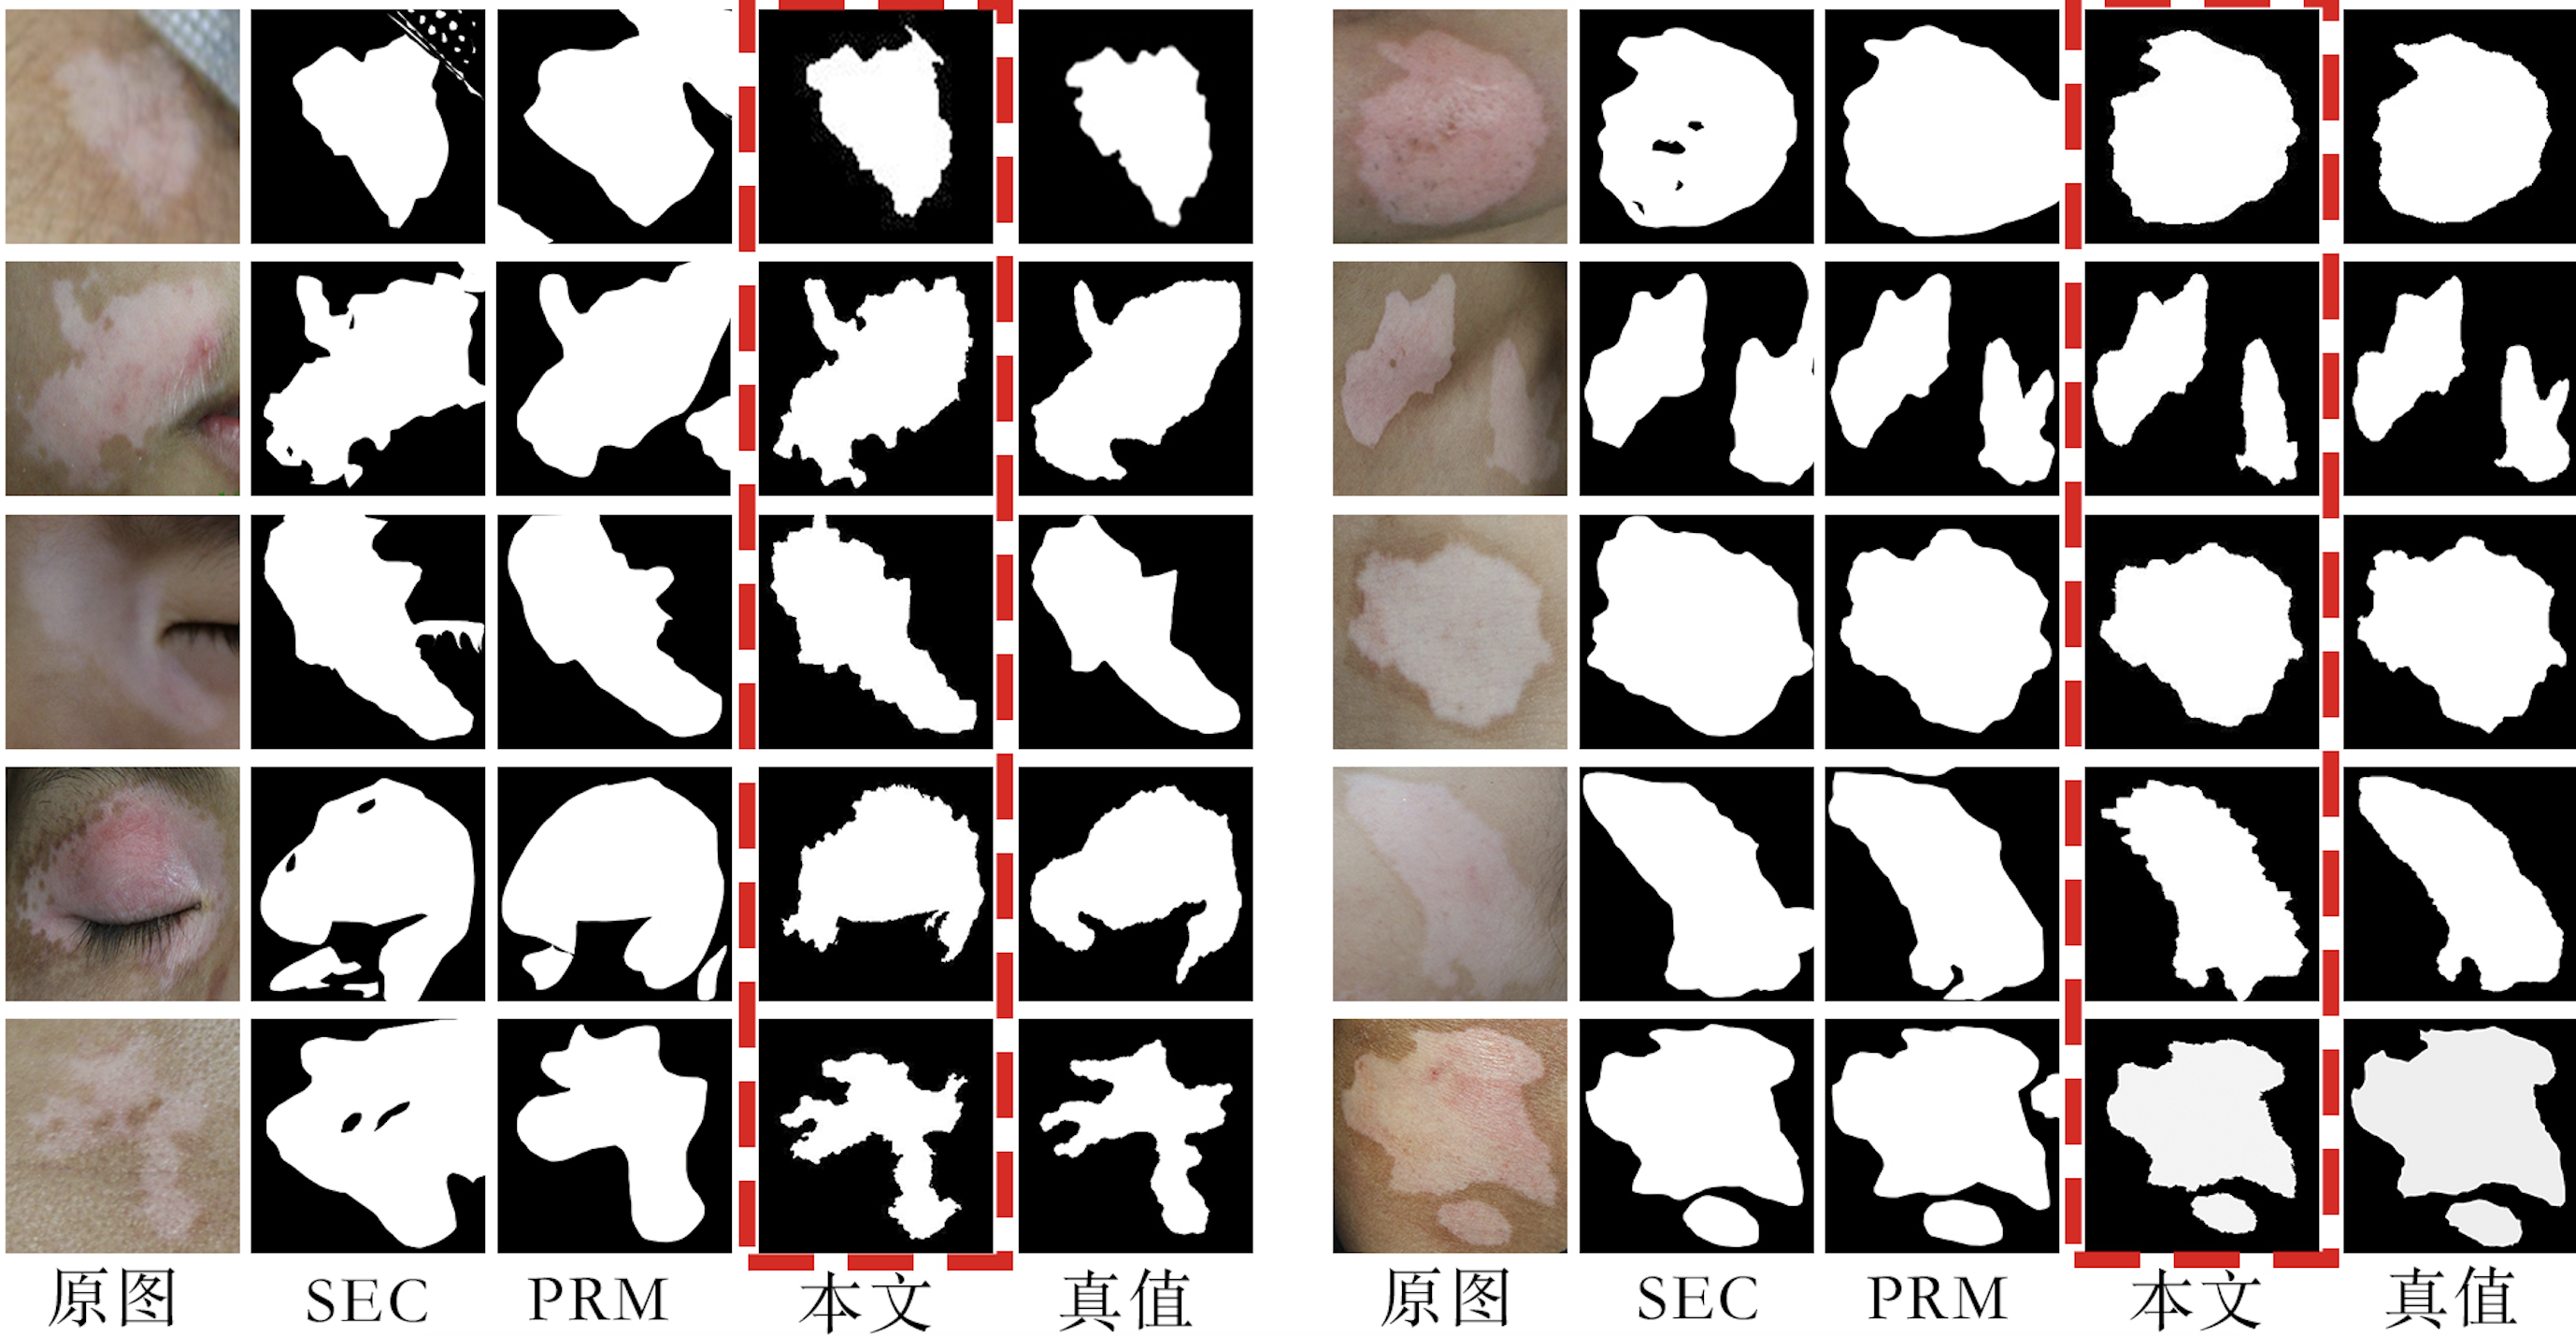
\includegraphics[width=\linewidth]{weaklySupervisedCompare.png}
\end{center}
   \caption{本文的方法与最先进的弱监督方法之间的视觉比较,即 SEC~\cite{Kolesnikov:2016tf} 和 PRM~\cite{Zhou:2018ul}. }\vspace{-3mm}
\label{fig:weaklySupervisedCompare}
\end{figure}

我们的失败的情况主要是由于在低对比度的情况下下,全局阈值$ {T_ \mathrm {bin}} $不恰当的设置(参见图\ref {fig:FailureCases})。然而,在真实的临床场景中,由于白癜风的性质,我们的显着图中的灰度级可以更好地代表皮损与健康皮肤之间的过渡区,并有助于评估不同程度的脱色素。此外,本文的方法有时会在强烈的光照条件下将正常皮肤误判为白癜风区域。

\begin{figure}[h]
\begin{center}
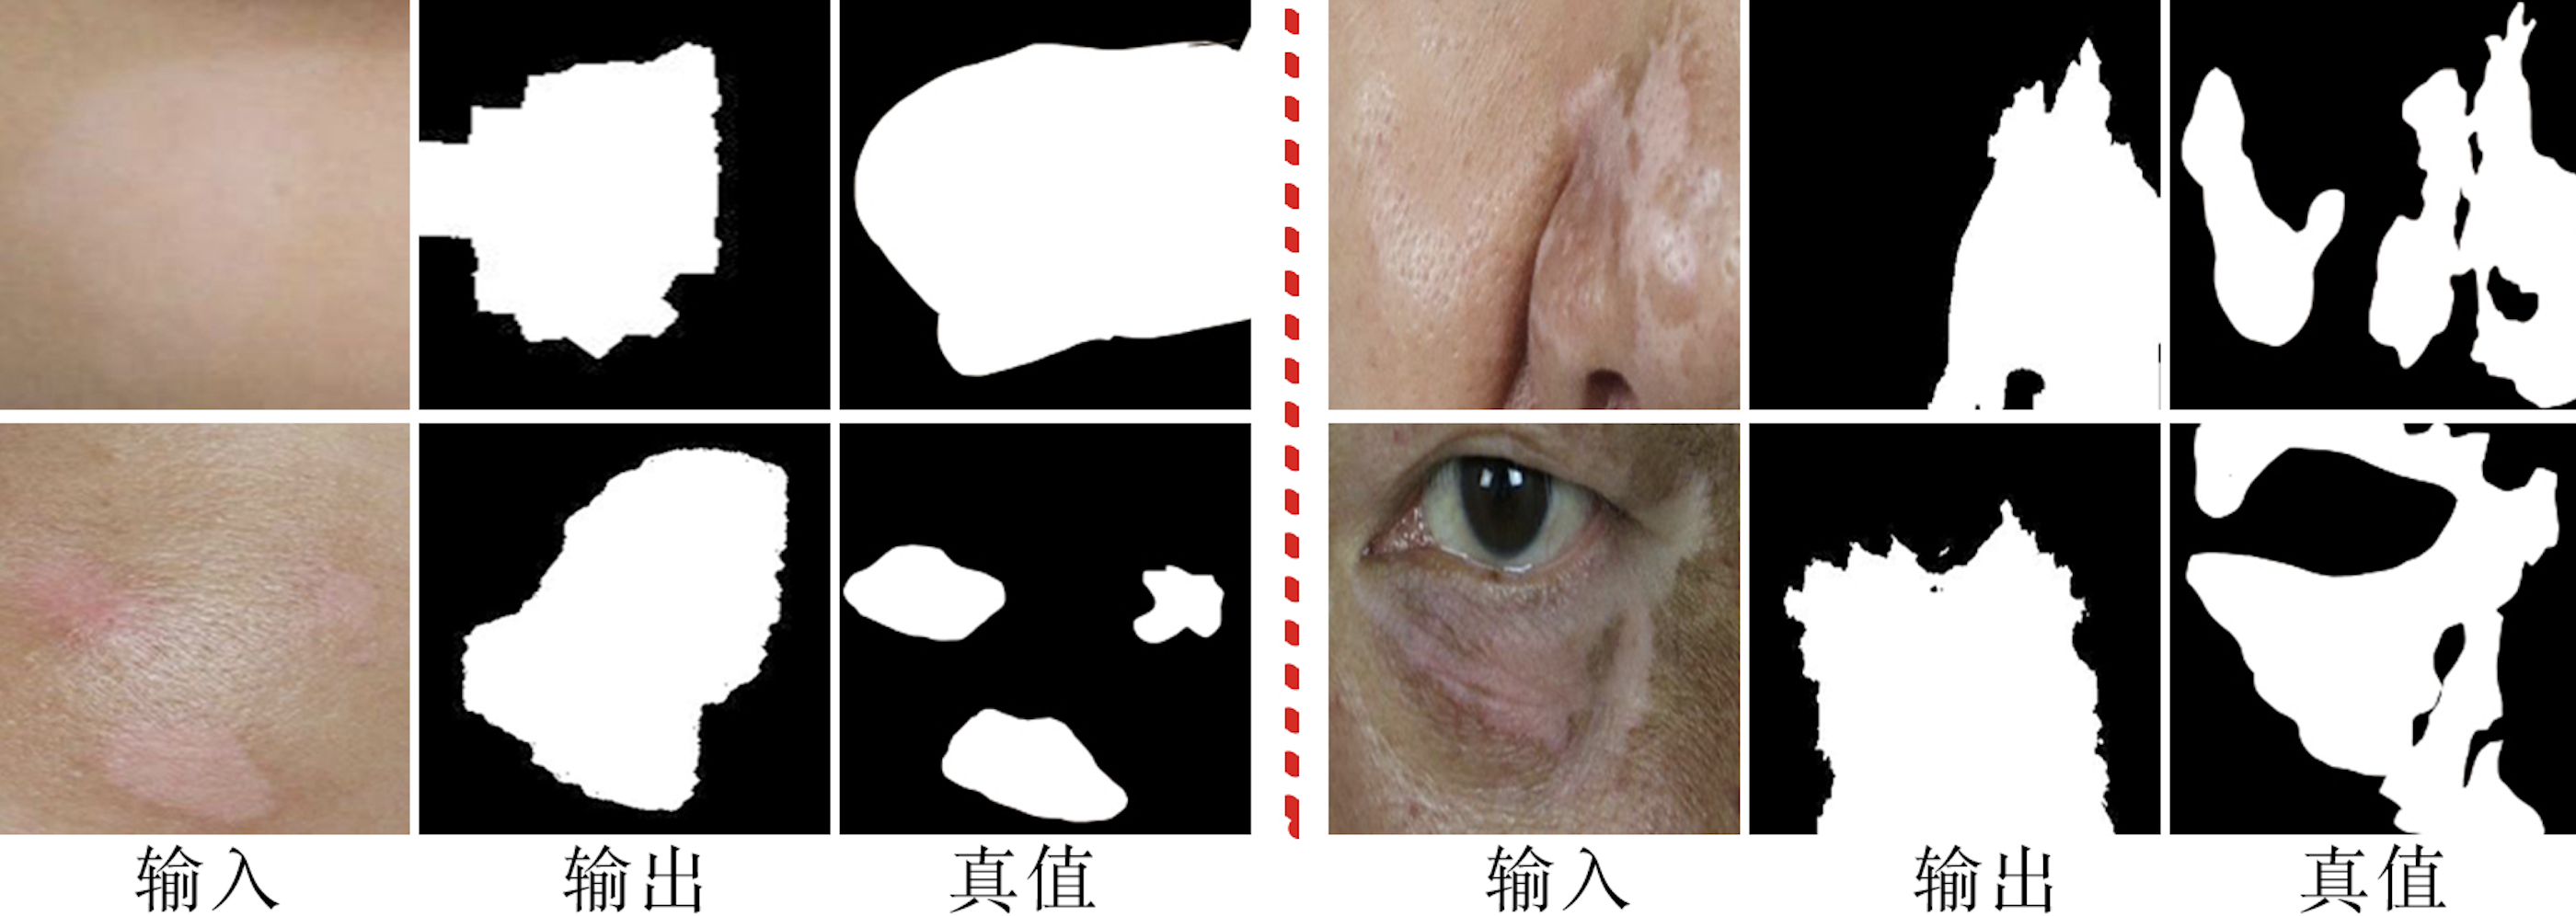
\includegraphics[width=\linewidth]{FailureCases.png}
\end{center}
   \caption{失败的案例}
\label{fig:FailureCases}
\end{figure}

\subsection{模型简化研究与敏感性测试}
\textbf{模型简化研究}


基于之前的介绍,本文总共引入了三个先验知识来帮助我们获得最终的显着性图,即前景蒙版,背景种子和边界种子。为了研究每个先验知识的贡献,我们在表4.2中探索了不同的组合所产生的结果。可以得出以下结论:

\begin{enumerate}
\item 当省略前景掩模和背景种子时,mIoU分别从71.4\%下降到62.5%和66.7\%,这表明激活图产生的先验的有效性。
\item 引入边界种子使性能提高了8.3\% 表明假设边界像素主要来自背景区域是有帮助的。
\item 当去掉三个先验中的两个时,mIoU从71.4\%急剧下降到59.5\%,43.5%和53.0\%,这表明三个先验是不可或缺的。
\item 当我们不使用最后一个显着性传播过程(同时丢弃前景掩码)并直接使用$ {T_ \mathrm {bin}} $来阈值分割$ S_\mathrm {Bnd} $和$ S_ \mathrm {Bg} $的乘法结果时,最终产生的二进制掩码与仅丢弃前景掩码相比IoU下降了4.8\%,这表明最后的显着性传播过程可以进一步提高显著图的质量。
\end{enumerate}

\begin{table}[htbp]
\label{tab:ablation}
\begin{center}
\caption{简化模型分析:针对不同的先验知识与显著性传播过程}
\setlength{\tabcolsep}{1 mm}{
    \begin{tabular}{c|cccccccc}
    \toprule
    Fg Mask & \xmark &   \cmark    &    \cmark   &   \cmark    & \xmark & \xmark & \xmark & \cmark \\
    Bg Seeds &  \cmark     & \xmark &   \cmark    & \xmark &  \cmark     & \xmark &  \cmark     & \cmark \\
    Bnd Seeds &  \cmark     &   \cmark    & \xmark & \xmark & \xmark &   \cmark    &   \cmark    & \cmark \\
    Last SP &   \cmark    &   \cmark    & \cmark      &   \cmark    &  \cmark     &    \cmark   &\xmark & \cmark \\
    \midrule
    mIoU  & 62.5  & 66.7  & 63.1  & 59.5  & 43.5  & 53.0  & 57.7  & \textbf{71.4}  \\
    \bottomrule
    \end{tabular}}%
\end{center}

  \label{tab:ablation}%
\end{table}%

\textbf{敏感性测试}

本文的算法中一共有五个参数需要手动调节,高斯核宽度$\theta$, 最大的超像素数量 ${N_\mathrm{max}}$, 二值化阈值 ${T_\mathrm{bin}}$,用于细化显著图的选择率 $\eta$ 以及用于获得前景与背景掩模的阈值对 $(T_\mathrm{f}$-$T_\mathrm{b})$ 。我们在此过程中使用控制变量法,在 $\mathrm{IoU}$意义下评估了每一个参数对模型的影响。图~\ref{fig:Sensitivity} 显示了本文的方法对于$\eta$ 和 ${N_\mathrm{max}}$的改变并不敏感,但是性能却非常依赖于 $\theta$的选择。 ${T_\mathrm{bin}}$ 的变化在以 $0.5$为中心的一个较大区间内变化均可以被接受。经过大量的实验,发现本文的方法具有很强的鲁棒性, 并且对于阈值对$(T_\mathrm{f}$-$T_\mathrm{b})$的选择在很大一个自由区间内仍然可以维持算法的有效性。经过测试,本文算法的最佳性能在取${T_\mathrm{b}}=30,{T_\mathrm{f}}=60$时达到。

\begin{figure}[htbp]
\begin{center}
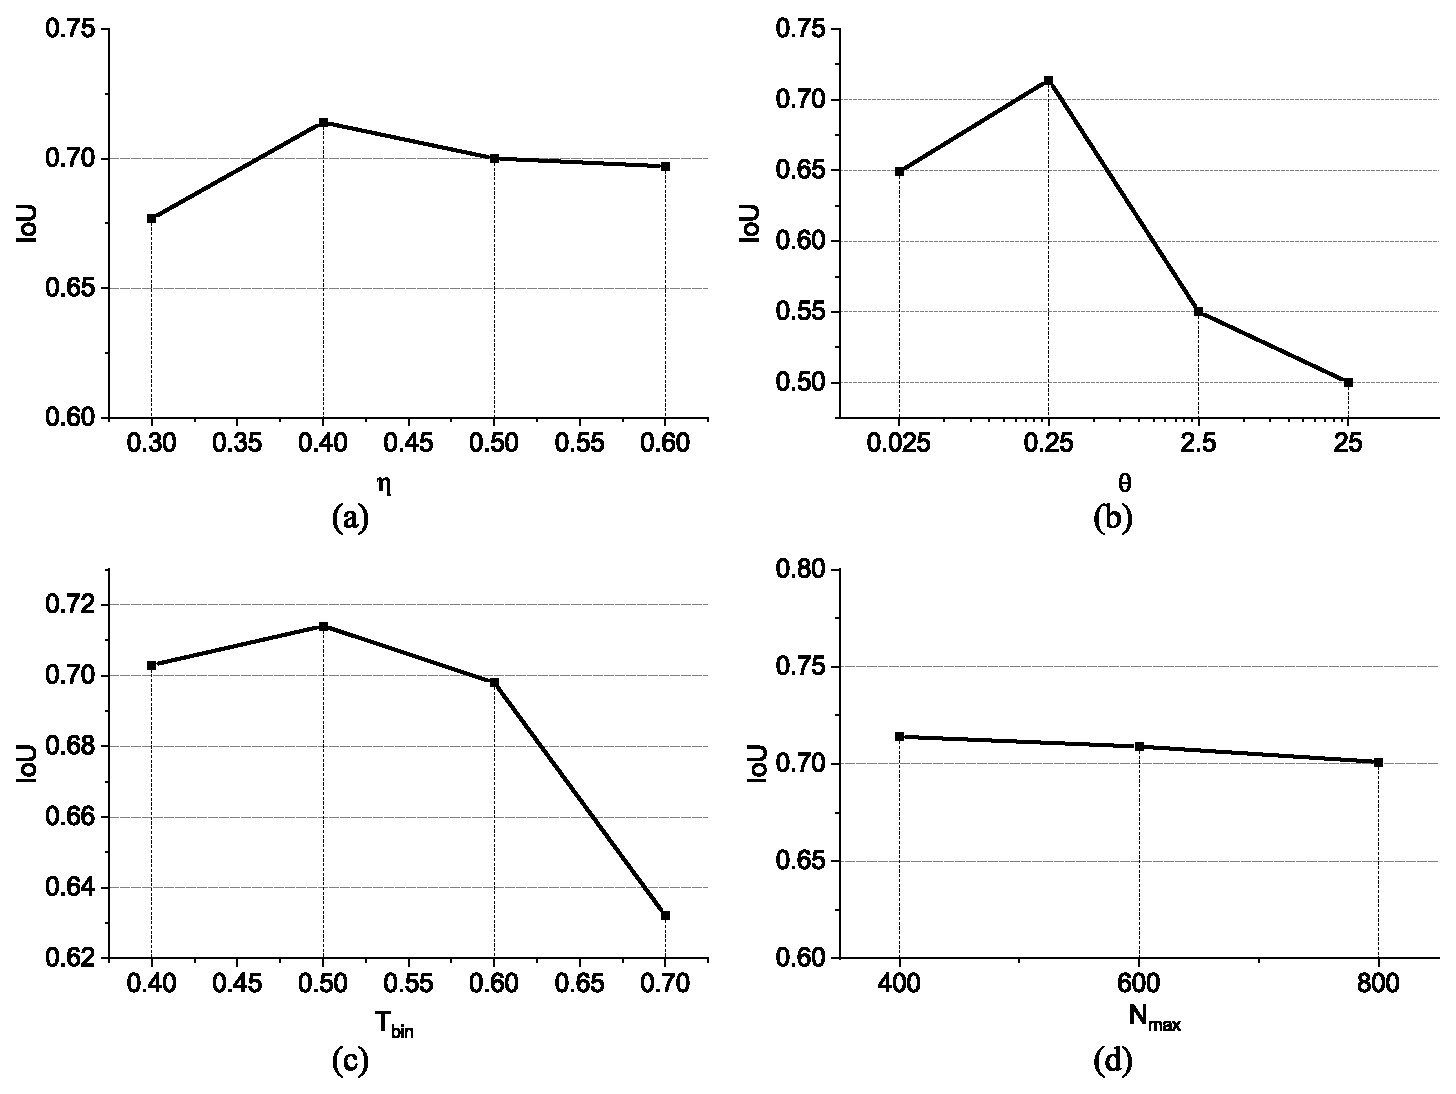
\includegraphics[width=0.7\linewidth]{composit1.eps}
\end{center}
   \caption{敏感性测试}
\label{fig:Sensitivity}
\end{figure}


\section{本章小结}
本章首先分析了在医疗图像处理领域对图像真值标注的困难性,然后引出了弱监督学习、弱监督分割的概念。然后提出了本文的核心方法并分别详细介绍了每一步骤中的原理以及意义,解释了如何做到“既见森林,又见树木”,解释了如何将反馈的思想应用到显著性传播的过程中,并说明了这种策略应用在白癜风分割领域所带来的好处。最后通过多个实验验证了该方法的有效性,并与强监督学习进行对比,发现在一些拍照环境恶劣,对比度很低的情况下,本文提出的方法可以更好的保持白癜风的边缘。




















\chapter{总结与展望}
\section{总结}
白斑面积是临床治疗白癜风效果的重要评价指标, 由于在评估方法上缺乏共识,这使得分析或比较不同研究的结果变得困难。而测量白斑面积的基础则是准确将白斑区域分割出来。

本文首先对现有的白癜风评价体方法展开充分的研究,进行了综合的对比,指出主观或半客观评价体系的缺点,并阐明了客观评价体系的必要性。就白斑分割方法而言,首先指出了分割在主观评价体系中的重要性,并从两个角度进行了相关工作的介绍,即色素性皮肤病分割与白癜风图像的分析与分割,并针对目前的所使用的方法进行了细致的原理分析和优缺点对比。分析得出了以白癜风为代表的色素性皮肤病所具有的特点及难点。

为了应对这些缺陷和难点,本文首先提出了到目前为止最大的一个白癜风数据集(Vit2019),此数据集拥有1000张来自临床和网络的白癜风图片,并且均进行了白癜风区域的像素级标注。而且本文从收集、标注、多样性与挑战四个方面详细介绍了该数据集,并举例分析了部分样例图片。这一数据集为之后的强监督分割与弱监督分割部分的效果评价提供了真值。

在对白癜风图像预处理的过程中,结合其图像对比度低、皮损与正常皮肤过渡区域模糊等特点,提出了使用超像素分割方法作为图像预处理步骤,从而达到降低维度、剔除异常像素点、保留较完整准确的皮损边界等三个目的;由于图像大小尺寸不一致,引出了经典超像素分割算法中初始种子点数目确定难的问题,并针对其提出了改进的方法。

对于强监督意义下的分割框架,本文着重介绍了一种经典的、具有代表性的网络结构——Unet,并且从定量和定性的角度展现并分 析了 Unet 在 Vit2019 上的效果。

对于弱监督分割框架,本章首先分析了在医疗图像处理领域对图像真值标注的困难性以及强监督分割所面临的限制。然后提出了本文的方法,并详细介绍了每一步骤中的原理以及意义,将 “既见森林,又见树木”的策略引入分割过程,使得该方法既可以从语义层面获得白癜风自身的特征,又可以从微观层面针对每一个患者的皮肤状况作出推理。而且在该方法中,我们结合了反馈的思想来控制显著性传播,使其可以根据不同情况自适应的调整传播过程。

最后通过多个实验验证了该弱监督分割框架的有效性,并与强监督学习的实验结果进行对比,发现在一些拍照环境恶劣,对比度很低的情况下,本文提出的方法甚至可以更好的分割白癜风区域并保持白癜风的边缘细节。

\section{展望}
本文提出的基于显著性传播的弱监督分割方法,在取得优良的性能的同时,也存在着局限性。由于临床拍摄环境的复杂,在某些极端情况下分割效果仍然难以尽如人意。例如在高光条件下或者当皮损区域位于人脸鼻侧附近,其崎岖的边界会对显著性传播造成一定的影响。另一方面,本文所提出的方法同样具有拓展到其他皮损区域分割的潜力,例如对黄褐斑、烧伤表皮进行分割。

未来在进行白癜风患病程度评价时,对于面积的计算可以采取两种策略,一是计算相对面积,二是计算绝对面积,此处以人脸处的白癜风面积为例,对未来的工作进行展望。计算相对面积,即通过分割方法得到掩模图像后,计算其中白色区域(白癜风)占整个图像区域的百分比;为了计算绝对面积,由于拍摄的角度不同,在二维图像中的白癜风区域受到了不同程度的形变,因此直接通过二维图像计算物理面积较不准确。因此,可以先通过3D建模技术构建人脸模型,然后将分割好的掩模图像投到人脸模型上,最终通过计算三角面片数来获得白癜风的物理面积。

通过对白癜风真实物理面积或者比例的计算,使得此模型更加完善,便于临床使用和推广。








%%% 其它部分
\backmatter

%% 本科生要这几个索引,研究生不要。选择性留下。
% 插图索引
%\listoffigures
% 表格索引
%\listoftables
% 公式索引
%\listofequations


%% 参考文献
% 注意:至少需要引用一篇参考文献,否则下面两行可能引起编译错误。
% 如果不需要参考文献,请将下面两行删除或注释掉。
\bibliographystyle{thuthesis-numeric}      % 顺序编码制
% \bibliographystyle{thuthesis-author-year}  % 著者-出版年制
% \bibliographystyle{thuthesis-bachelor}     % 本科生参考文献的著录格式
\bibliography{ref/refs}


%% 致谢
% 如果使用声明扫描页,将可选参数指定为扫描后的 PDF 文件名,例如:
% \begin{acknowledgement}[scan-statement.pdf]
\begin{acknowledgement}
首先感谢夏思宇老师对该论文从选题,构思到最后定稿的各个环节给予细心指引与教导。在每周的交流与讨论中,总可以从夏老师的讲解与解答中学习到新的知识。在遇到困难时,夏老师不但会给出可能的解决思路,也会启发式地鼓励我去寻找解决方法。讨论遇到分歧时,夏老师也同样会尊重我的意见。

这大学四年中还得到众多老师的关心支持和帮助。在此,谨向老师们致以衷心的感谢和崇高的敬意。

感谢父母的关心,不断地为我提供前行的动力。

最后,向参与评审与答辩的老师们表示感谢。
\end{acknowledgement}


%% 附录
%\begin{appendix}
%\chapter{外文资料原文}
\label{cha:engorg}

\title{The title of the English paper}

\textbf{Abstract:} As one of the most widely used techniques in operations
research, \emph{ mathematical programming} is defined as a means of maximizing a
quantity known as \emph{bjective function}, subject to a set of constraints
represented by equations and inequalities. Some known subtopics of mathematical
programming are linear programming, nonlinear programming, multiobjective
programming, goal programming, dynamic programming, and multilevel
programming$^{[1]}$.

It is impossible to cover in a single chapter every concept of mathematical
programming. This chapter introduces only the basic concepts and techniques of
mathematical programming such that readers gain an understanding of them
throughout the book$^{[2,3]}$.


\section{Single-Objective Programming}
The general form of single-objective programming (SOP) is written
as follows,
\begin{equation*} % 如果附录中的公式不想让它出现在公式索引中,那就请
                             % 用 equation*
\left\{\begin{array}{l}
\max \,\,f(x)\\[0.1 cm]
\mbox{subject to:} \\ [0.1 cm]
\qquad g_j(x)\le 0,\quad j=1,2,\cdots,p
\end{array}\right.
\end{equation*}
which maximizes a real-valued function $f$ of
$x=(x_1,x_2,\cdots,x_n)$ subject to a set of constraints.

\newcommand\Real{\mathbf{R}}
\newtheorem{mpdef}{Definition}[chapter]
\begin{mpdef}
In SOP, we call $x$ a decision vector, and
$x_1,x_2,\cdots,x_n$ decision variables. The function
$f$ is called the objective function. The set
\begin{equation*}
S=\left\{x\in\Real^n\bigm|g_j(x)\le 0,\,j=1,2,\cdots,p\right\}
\end{equation*}
is called the feasible set. An element $x$ in $S$ is called a
feasible solution.
\end{mpdef}

\newtheorem{mpdefop}[mpdef]{Definition}
\begin{mpdefop}
A feasible solution $x^*$ is called the optimal
solution of SOP if and only if
\begin{equation}
f(x^*)\ge f(x)
\end{equation}
for any feasible solution $x$.
\end{mpdefop}

One of the outstanding contributions to mathematical programming was known as
the Kuhn-Tucker conditions\ref{eq:ktc}. In order to introduce them, let us give
some definitions. An inequality constraint $g_j(x)\le 0$ is said to be active at
a point $x^*$ if $g_j(x^*)=0$. A point $x^*$ satisfying $g_j(x^*)\le 0$ is said
to be regular if the gradient vectors $\nabla g_j(x)$ of all active constraints
are linearly independent.

Let $x^*$ be a regular point of the constraints of SOP and assume that all the
functions $f(x)$ and $g_j(x),j=1,2,\cdots,p$ are differentiable. If $x^*$ is a
local optimal solution, then there exist Lagrange multipliers
$\lambda_j,j=1,2,\cdots,p$ such that the following Kuhn-Tucker conditions hold,
\begin{equation}
\label{eq:ktc}
\left\{\begin{array}{l}
    \nabla f(x^*)-\sum\limits_{j=1}^p\lambda_j\nabla g_j(x^*)=0\\[0.3cm]
    \lambda_jg_j(x^*)=0,\quad j=1,2,\cdots,p\\[0.2cm]
    \lambda_j\ge 0,\quad j=1,2,\cdots,p.
\end{array}\right.
\end{equation}
If all the functions $f(x)$ and $g_j(x),j=1,2,\cdots,p$ are convex and
differentiable, and the point $x^*$ satisfies the Kuhn-Tucker conditions
(\ref{eq:ktc}), then it has been proved that the point $x^*$ is a global optimal
solution of SOP.

\subsection{Linear Programming}
\label{sec:lp}

If the functions $f(x),g_j(x),j=1,2,\cdots,p$ are all linear, then SOP is called
a {\em linear programming}.

The feasible set of linear is always convex. A point $x$ is called an extreme
point of convex set $S$ if $x\in S$ and $x$ cannot be expressed as a convex
combination of two points in $S$. It has been shown that the optimal solution to
linear programming corresponds to an extreme point of its feasible set provided
that the feasible set $S$ is bounded. This fact is the basis of the {\em simplex
  algorithm} which was developed by Dantzig as a very efficient method for
solving linear programming.
\begin{table}[ht]
\centering
  \centering
  \caption*{Table~1\hskip1em This is an example for manually numbered table, which
    would not appear in the list of tables}
  \label{tab:badtabular2}
  \begin{tabular}[c]{|m{1.5cm}|c|c|c|c|c|c|}\hline
    \multicolumn{2}{|c|}{Network Topology} & \# of nodes &
    \multicolumn{3}{c|}{\# of clients} & Server \\\hline
    GT-ITM & Waxman Transit-Stub & 600 &
    \multirow{2}{2em}{2\%}&
    \multirow{2}{2em}{10\%}&
    \multirow{2}{2em}{50\%}&
    \multirow{2}{1.2in}{Max. Connectivity}\\\cline{1-3}
    \multicolumn{2}{|c|}{Inet-2.1} & 6000 & & & &\\\hline
    \multirow{2}{1.5cm}{Xue} & Rui  & Ni &\multicolumn{4}{c|}{\multirow{2}*{\thuthesis}}\\\cline{2-3}
    & \multicolumn{2}{c|}{ABCDEF} &\multicolumn{4}{c|}{} \\\hline
\end{tabular}
\end{table}

Roughly speaking, the simplex algorithm examines only the extreme points of the
feasible set, rather than all feasible points. At first, the simplex algorithm
selects an extreme point as the initial point. The successive extreme point is
selected so as to improve the objective function value. The procedure is
repeated until no improvement in objective function value can be made. The last
extreme point is the optimal solution.

\subsection{Nonlinear Programming}

If at least one of the functions $f(x),g_j(x),j=1,2,\cdots,p$ is nonlinear, then
SOP is called a {\em nonlinear programming}.

A large number of classical optimization methods have been developed to treat
special-structural nonlinear programming based on the mathematical theory
concerned with analyzing the structure of problems.
\begin{figure}[h]
  \centering
  \includegraphics{thu-lib-logo.pdf}
  \caption*{Figure~1\quad This is an example for manually numbered figure,
    which would not appear in the list of figures}
  \label{tab:badfigure2}
\end{figure}

Now we consider a nonlinear programming which is confronted solely with
maximizing a real-valued function with domain $\Real^n$.  Whether derivatives are
available or not, the usual strategy is first to select a point in $\Real^n$ which
is thought to be the most likely place where the maximum exists. If there is no
information available on which to base such a selection, a point is chosen at
random. From this first point an attempt is made to construct a sequence of
points, each of which yields an improved objective function value over its
predecessor. The next point to be added to the sequence is chosen by analyzing
the behavior of the function at the previous points. This construction continues
until some termination criterion is met. Methods based upon this strategy are
called {\em ascent methods}, which can be classified as {\em direct methods},
{\em gradient methods}, and {\em Hessian methods} according to the information
about the behavior of objective function $f$. Direct methods require only that
the function can be evaluated at each point. Gradient methods require the
evaluation of first derivatives of $f$. Hessian methods require the evaluation
of second derivatives. In fact, there is no superior method for all
problems. The efficiency of a method is very much dependent upon the objective
function.

\subsection{Integer Programming}

{\em Integer programming} is a special mathematical programming in which all of
the variables are assumed to be only integer values. When there are not only
integer variables but also conventional continuous variables, we call it {\em
  mixed integer programming}. If all the variables are assumed either 0 or 1,
then the problem is termed a {\em zero-one programming}. Although integer
programming can be solved by an {\em exhaustive enumeration} theoretically, it
is impractical to solve realistically sized integer programming problems. The
most successful algorithm so far found to solve integer programming is called
the {\em branch-and-bound enumeration} developed by Balas (1965) and Dakin
(1965). The other technique to integer programming is the {\em cutting plane
  method} developed by Gomory (1959).

\hfill\textit{Uncertain Programming\/}\quad(\textsl{BaoDing Liu, 2006.2})

\section*{References}
\noindent{\itshape NOTE: These references are only for demonstration. They are
  not real citations in the original text.}

\begin{translationbib}
\item Donald E. Knuth. The \TeX book. Addison-Wesley, 1984. ISBN: 0-201-13448-9
\item Paul W. Abrahams, Karl Berry and Kathryn A. Hargreaves. \TeX\ for the
  Impatient. Addison-Wesley, 1990. ISBN: 0-201-51375-7
\item David Salomon. The advanced \TeX book.  New York : Springer, 1995. ISBN:0-387-94556-3
\end{translationbib}

\chapter{外文资料的调研阅读报告或书面翻译}

\title{英文资料的中文标题}

{\heiti 摘要:} 本章为外文资料翻译内容。如果有摘要可以直接写上来,这部分好像没有
明确的规定。

\section{单目标规划}
北冥有鱼,其名为鲲。鲲之大,不知其几千里也。化而为鸟,其名为鹏。鹏之背,不知其几
千里也。怒而飞,其翼若垂天之云。是鸟也,海运则将徙于南冥。南冥者,天池也。
\begin{equation}\tag*{(123)}
 p(y|\mathbf{x}) = \frac{p(\mathbf{x},y)}{p(\mathbf{x})}=
\frac{p(\mathbf{x}|y)p(y)}{p(\mathbf{x})}
\end{equation}

吾生也有涯,而知也无涯。以有涯随无涯,殆已!已而为知者,殆而已矣!为善无近名,为
恶无近刑,缘督以为经,可以保身,可以全生,可以养亲,可以尽年。

\subsection{线性规划}
庖丁为文惠君解牛,手之所触,肩之所倚,足之所履,膝之所倚,砉然响然,奏刀騞然,莫
不中音,合于桑林之舞,乃中经首之会。
\begin{table}[ht]
\centering
  \centering
  \caption*{表~1\hskip1em 这是手动编号但不出现在索引中的一个表格例子}
  \label{tab:badtabular3}
  \begin{tabular}[c]{|m{1.5cm}|c|c|c|c|c|c|}\hline
    \multicolumn{2}{|c|}{Network Topology} & \# of nodes &
    \multicolumn{3}{c|}{\# of clients} & Server \\\hline
    GT-ITM & Waxman Transit-Stub & 600 &
    \multirow{2}{2em}{2\%}&
    \multirow{2}{2em}{10\%}&
    \multirow{2}{2em}{50\%}&
    \multirow{2}{1.2in}{Max. Connectivity}\\\cline{1-3}
    \multicolumn{2}{|c|}{Inet-2.1} & 6000 & & & &\\\hline
    \multirow{2}{1.5cm}{Xue} & Rui  & Ni &\multicolumn{4}{c|}{\multirow{2}*{\thuthesis}}\\\cline{2-3}
    & \multicolumn{2}{c|}{ABCDEF} &\multicolumn{4}{c|}{} \\\hline
\end{tabular}
\end{table}

文惠君曰:“嘻,善哉!技盖至此乎?”庖丁释刀对曰:“臣之所好者道也,进乎技矣。始臣之
解牛之时,所见无非全牛者;三年之后,未尝见全牛也;方今之时,臣以神遇而不以目视,
官知止而神欲行。依乎天理,批大郤,导大窾,因其固然。技经肯綮之未尝,而况大坬乎!
良庖岁更刀,割也;族庖月更刀,折也;今臣之刀十九年矣,所解数千牛矣,而刀刃若新发
于硎。彼节者有间而刀刃者无厚,以无厚入有间,恢恢乎其于游刃必有余地矣。是以十九年
而刀刃若新发于硎。虽然,每至于族,吾见其难为,怵然为戒,视为止,行为迟,动刀甚微,
謋然已解,如土委地。提刀而立,为之而四顾,为之踌躇满志,善刀而藏之。”

文惠君曰:“善哉!吾闻庖丁之言,得养生焉。”


\subsection{非线性规划}
孔子与柳下季为友,柳下季之弟名曰盗跖。盗跖从卒九千人,横行天下,侵暴诸侯。穴室枢
户,驱人牛马,取人妇女。贪得忘亲,不顾父母兄弟,不祭先祖。所过之邑,大国守城,小
国入保,万民苦之。孔子谓柳下季曰:“夫为人父者,必能诏其子;为人兄者,必能教其弟。
若父不能诏其子,兄不能教其弟,则无贵父子兄弟之亲矣。今先生,世之才士也,弟为盗
跖,为天下害,而弗能教也,丘窃为先生羞之。丘请为先生往说之。”
\begin{figure}[h]
  \centering
  \includegraphics{thu-whole-logo.pdf}
  \caption*{图~1\hskip1em 这是手动编号但不出现索引中的图片的例子}
  \label{tab:badfigure3}
\end{figure}

柳下季曰:“先生言为人父者必能诏其子,为人兄者必能教其弟,若子不听父之诏,弟不受
兄之教,虽今先生之辩,将奈之何哉?且跖之为人也,心如涌泉,意如飘风,强足以距敌,
辩足以饰非。顺其心则喜,逆其心则怒,易辱人以言。先生必无往。”

孔子不听,颜回为驭,子贡为右,往见盗跖。

\subsection{整数规划}
盗跖乃方休卒徒大山之阳,脍人肝而餔之。孔子下车而前,见谒者曰:“鲁人孔丘,闻将军
高义,敬再拜谒者。”谒者入通。盗跖闻之大怒,目如明星,发上指冠,曰:“此夫鲁国之
巧伪人孔丘非邪?为我告之:尔作言造语,妄称文、武,冠枝木之冠,带死牛之胁,多辞缪
说,不耕而食,不织而衣,摇唇鼓舌,擅生是非,以迷天下之主,使天下学士不反其本,妄
作孝弟,而侥幸于封侯富贵者也。子之罪大极重,疾走归!不然,我将以子肝益昼餔之膳。”


\chapter{其它附录}
前面两个附录主要是给本科生做例子。其它附录的内容可以放到这里,当然如果你愿意,可
以把这部分也放到独立的文件中,然后将其 \cs{input} 到主文件中。

%\end{appendix}

%% 个人简历
\begin{resume}

  \researchitem{学术论文} % 发表的和录用的合在一起

  % 1. 已经刊载的学术论文(本人是第一作者,或者导师为第一作者本人是第二作者)
  \begin{publications}
    \item Zhangxing Bian, Siyu Xia, Chao Xia, Ming Shao, FU YUN. Weakly Supervised Vitiligo Segmentation in Skin Image through Saliency
Propagation. \textit{In Proceedings of the IEEE international conference on computer vision}, 2019. (于2019年3月投稿)
    \end{publications}

 
  \researchitem{申请专利成果} % 有就写,没有就删除
  \begin{achievements}
    \item 已提交申请专利《一种简单高效的白癜风皮损区域分割方法》;发明人:边张行,夏思宇;申请人:东南大学;公开号:CN 109741336 A 
  \end{achievements}

\end{resume}


%% 本科生进行格式审查是需要下面这个表格,答辩可能不需要。选择性留下。
% 综合论文训练记录表
%\includepdf[pages=-]{scan-record.pdf}
\end{document}
